\documentclass[
12pt         % Moar bigger
,twoside     % fogs hates this, but they hate everything
,openright   % fogs hates this too
]{mythesis}

% I used these in my thesis.  They're useful.  booktabs makes non-shit
% tables.
\usepackage{graphicx}
\usepackage{amsmath}
\usepackage{booktabs}

\title{The genetic interactions  \\%
  of effective population size,  \\ mutation, and migration}

%\title{Effective population size \\%
%  and its interactions with \\ population genetic processes}
  % alternate title with adaptree version? Population genetics in a changing world: Understanding local adaptation and effective population sizes in the face of complex demographic history
%
\author{Kimberly Julie Gilbert}
%
\month{\textsc{november}} \year{2016}
\previousdegrees{B.Sc., University of Virginia, 2010}
\degreetitle{Doctor of Philosophy}
\department{Zoology}

\begin{document}

\maketitle

% I worked in different files: input them like so:

\chapter*{Abstract}
\chaptermark{abstract}
\addcontentsline{toc}{chapter}{Abstract}

%% 362 currently
Evolution is driven by four major processes that create, maintain, or eliminate genetic diversity within and among populations: mutation, gene flow, genetic drift, and natural selection. My thesis examines the role of demographic history and its impact on the evolution of populations through interacting with each of these processes. Demographic history can cause populations to exist in various states of non-equilibria which has the potential to mis-inform important evolutionary inferences. Such inferences may be key in applied biology where conservation decisions must be made. I begin with a study on the estimation of effective population sizes under the assumption-violating scenario of migration among populations (\Chapref{effectivepopsize}). Effective population size is proportional to the amount of genetic drift a population experiences, yet the presence of gene flow can affect measures of drift and thus estimates of population size. I have tested existing estimation methods using simulated data to understand the impact of migration on estimation accuracy. I next present two studies on species range expansions and the roles of migration, mutation, and selection on expansion dynamics. Range expansions are a common occurrence in many species and a major case of non-equilibrium demographic history. The first of these studies examines the ability of species to expand over patches of environmental optima under different genetic architecture regimes (\Chapref{heterogeneouslandscapes}). Expansion is enhanced by different forms of genetic architecture, and each of these interacts with the size of patches on the landscape as well as how strongly selection varies across patches. \Chapref{expansionload} explores the interaction of fitness reductions due to deleterious mutations and due to local maladaptation to the environment during range expansions. The interplay of expansion load, mutation load, and migration load lead to different levels of local adaptation in expanding populations. My final study assesses the reproducibility of analyses using the common algorithm \textsc{structure} (\Chapref{reproducibility}). This research investigates the ability to regenerate results from this stochastic analysis method using published datasets, and elucidates the reasons for cases where reproducibility failed. In sum, my thesis contributes to our understanding of how gene flow, population size, landscape heterogeneity, and mutation interact to impact the genetics of populations and thus the fate of evolving biodiversity.

%%% Local Variables:
%%% TeX-master: "thesis"
%%% TeX-PDF-mode: t
%%% End:


%% MUST BE < 350 WORDS
%% MUST BE ON PAGE ii

%% NO ABSTRACTS WITHIN CHAPTERS

%% 428 words :/
%% Evolution is driven by four major processes: mutation, gene flow, genetic drift, and natural selection. Each of these plays a major role in determining the future of species and whether populations will adapt and survive or go extinct. My thesis addresses each these processes through examining the role of demographic history and its impact on the evolution of populations. Demographic history can cause populations to exist in various states of non-equilibria which has the potential to mis-inform important evolutionary inferences. Such inferences may be key in applied biology where conservation decisions must be made. I begin my investigations of this effect of demographic history with a study on the estimation of effective population sizes under the non-equilibrium, assumption-violating scenario of migration among populations (\Chapref{effectivepopsize}). Effective population size is proportional to the amount of genetic drift a population experiences, yet the presence of gene flow can affect measures of drift and thus estimates of population size. I have tested existing estimation methods using simulated data to understand the impact of migration on accuracy of estimates. I next present two studies on species range expansions and the roles of migration, mutation, and selection on expansion dynamics. Range expansions are a common occurrence in many species and a major case of non-equilibrium demographic history. The first of these studies examines the ability of species to expand over heterogeneously changing environmental optima under different genetic architecture regimes (\Chapref{heterogeneouslandscapes}). Expansion requires that edge populations adapt to new conditions, but with the added condition of colonization occurring from edge populations of smaller effective population sizes where the strength of selection is reduced. Adaptation during expansion becomes easier with larger patches of the same selective pressures, but adaptation and expansion are inhibited on very patchy landscapes if selection varies greatly across patches. The second of these studies explores the actions and interactions of fitness reductions due to deleterious mutations and due to local maladaptation to the environment on populations at the expanding edge of a species range (\Chapref{expansionload}). This interplay of expansion load, mutation load, and migration load lead to different levels of local adaptation in expanding populations. My final study assesses the reproducibility of analyses using the common algorithm \textsc{structure} (\Chapref{reproducibility}). This research investigates the ability of stochastic genetic analysis methods to recreate identical results from the same data, and elucidates the reasons for cases where reproducibility failed. In sum, my thesis contributes to our understanding of how gene flow, population size, landscape heterogeneity, and mutation interact and impact the genetics of populations and thus the fate of evolving biodiversity.


\chapter*{Preface}
\addcontentsline{toc}{chapter}{Preface}


\lettherebespace
\textsc{\Chapref{effectivepopsize}} has been previously published as:
%
\begin{previouspaper}
  Gilbert K.J. and Whitlock M.C. 2015. Evaluating methods for estimating local effective 
  population size with and without migration. \emph{Evolution}, 68:2154-2166.
\end{previouspaper}
%
Michael C. Whitlock helped formulate the project idea, provided guidance, writing, and editing.

\lettherebespace
\textsc{\Chapref{expansionload}} has been submitted for publication. % \emph{The American Naturalist}. 
I was primary author on this work and conducted all of the simulations and analyses the majority of writing. This work was coauthored with Nathaniel P. Sharp, Amy L. Angert, Gina L. Conte, Jeremy A. Draghi, Fr\'ed\'eric Guillaume, Anna L. Hargreaves, Remi Matthey-Doret, and Michael C. Whitlock.

\lettherebespace
\textsc{\Chapref{heterogeneouslandscapes}} was coauthored with Michael C. Whitlock. I was the primary author with guidance from Michael C. Whitlock.

\lettherebespace
\textsc{\Chapref{reproducibility}} has been previously published as:
%
\begin{previouspaper}
  Gilbert K.J., Andrew R.L., Bock D.G., Franklin M.T., Kane N.C., Moore J-S., Moyers B.T., Renaut S., Rennison D.J., Veen T., and Vines T.H. 2012. Recommendations for utilizing and reporting population genetic analyses: The reproducibility of genetic clustering using the program \sc{structure}. \emph{Molecular Ecology}, 21:4925-4930.
\end{previouspaper}
%
Timothy H. Vines formulated the initial project idea. All authors performed data reanalyses. I was the primary author.

%%% Local Variables:
%%% mode: latex
%%% TeX-master: "thesis"
%%% TeX-PDF-mode: t
%%% End:

% This is because FoGS formatting pedandtry is especially accute when
% it comes to tables of contents
\allcontents
% There is currently a problem with spacing somewhere so that Table of
% Contents, List of Tables, and List of Figures have the wrong amount
% of space.  Others are OK though...
\chapter*{Acknowledgements}
\addcontentsline{toc}{chapter}{Acknowledgements}

My greatest thanks goes to my advisor, Mike Whitlock. Mike has been a fantastic mentor and provided me with endless support both scientifically and academically. His thoughtful insight has been critical in the completion of the work presented herein. Mike's ability to not only teach the intricacies of all aspects of population genetics in depth, but to also enlighten me on the most tangential facts of life has made working under his supervision a great pleasure and a truly educational experience. I also thank the members of my advisory committee: Amy Angert, Loren Rieseberg, and Sally Aitken. Their helpful feedback, discussions, and support greatly improved my research.

Working amongst other members of the Otto-Whitlock labs and the UBC biodiversity research group not only made for a fantastic work environment, but also provided motivational support and vast resources of knowledge and skills. I am honored to thank these people for the knowledge and wisdom they have imparted and thankful to have gained many lifelong friends and colleagues. In particular, I would like to thank Rich FitzJohn for teaching me many of the intricacies of the R language, as well as the value of good graphic design. Jeremy Draghi, who taught me C and C++, was always a great source of calm sensibility when I felt lost. Florence D\'ebarre was an outstanding mentor who imparted deep understanding of mathematical biology in the most lighthearted manner. I owe thanks to many people, both near and far, friends and family, for support at the best and worst of times -- Katie Lotterhos, Sam Yeaman, Holly Kindsvater, Matt Pennell, Michael Scott, Nathaniel Sharp, Matt Osmond, Jasmine Ono, Liz Kleynhans, Thor Veen, Carl Rothfels, Tim Vines, Diana Rennison, Aleeza Gerstein, Kay Hodgins, Julie Lee-Yaw, Seth Rudman, Amanda Moreira, Chett Hopkins, Cathy Rushworth, and Peter Fields.

Despite the absence of a chapter on local adaptation in lodgepole pine, a large portion of time during my PhD was spent on forthcoming work which would not be possible without the help of numerous people. Sally Aitken was an expert on all things trees and provided connections and support, as well as a great field vehicle. Nick Ukrainetz and Vicky Berger with the BC Ministry of Forests provided me with all details and data on the Illingworth provenance trials. I had two amazing field assistants, Evan Cronmiller and Warren Neuvonen, who were both hard-working and fun. They always managed to keep a smile on my face despite the long, hot, bug-, and pollen-filled days spent in the forests of British Columbia. Anne Berland provided excellent experience and navigational skills for visiting the Illingworth provenance trials. Stilianos Louca helped me collect additional samples of lodgepole pine from northern BC and the Yukon. Katie Lotterhos, Chett Hopkins, Roxy, Florence D\'ebarre, Holly Kindsvater, and Jeremy Draghi all also contributed their own time to help me at various times in the field. Kristin Nurkowski was my trusted expert in the wet lab, seeing me through troubleshooting DNA extractions and devising solutions to all of the difficulties that arise in the lab. I have a newfound appreciation for bunnies and a clean centrifuge thanks to Kristin. I also thank all of the members of the AdapTree team and Sally Aitken's lab.

Compute Canada and Westgrid were essential resources without which this research would not have been possible. I thank Fr\'ed\'eric Guillaume for all of his time and help explaining and tinkering in \textsc{nemo}.

This work was financially supported by a BRITE Fellowship, UBC Affiliated Fellowships, a Zoology Graduate Fellowship, and an NSERC Discovery Grant. 
%%% Local Variables:
%%% TeX-master: "thesis.tex"
%%% TeX-PDF-mode: t
%%% End:

\cleardoublepage
\phantomsection
\addcontentsline{toc}{chapter}{Dedication}
\vspace*{.1\textheight}
\begin{center}
  To my parents, who fostered my love of science and the outdoors \\ throughout my entire life.
\end{center}

\cleardoublepage
\mainbody

\chapter{Introduction}
\label{chap:introduction}

% Yay inspiriational quotes.
\begin{quoteshrink}
% alternate quote: "The change from one stable equilibrium to the other may take place as the result of the isolation of a small unrepresentative group of the population, a temporary change in the environment which alters the relative viability of different types, or in several other ways..."
  ``I do not propose to argue the case for evolution, which I regard as being quite as well proven as most other historical facts, but to discuss its possible causes, which are certainly debatable.''
  \hfill\citet{Haldane:1932}, p.3
\end{quoteshrink}
% A Review of Some Fundamental Concepts and Problems of Population Genetics', Cold Spring Harbor Symposia on Quantitative Biology, 1955, 20, 13-14

\noindent


% aim for 8-9 pages?

The study of evolution aims to understand the myriads of diversity in existence today, how they came to be, and why. An essential part of this task requires understanding the genetic processes and patterns that occur in and define populations. Population genetics coalesced as a field in the early 1900s, following more than a decade of controversy and debate over the process of evolution \citep{Provine:2001}. Since its advent, great insight has been made into the processes that contribute to the evolution of populations and species. Our understandings of genetic drift, gene flow, mutation, and selection have created a solid foundation for the growing field of evolutionary biology. Yet as the field has advanced, the realization that the manifold and minute complexities of these processes can immensely impact populations and species has left open questions in the field of evolutionary biology.

One of the interesting complexities in understanding population genetics is the role of demographic history. Though population genetics eponymously (FIX THAT WORD) uses genetic data both in theory and empirically to understand the process of evolution, informing such genetic data with demographic information is often, if not always, necessary. Without this combination of information, it is nearly impossible to gain a full understanding of the ancestral processes leading to the system at hand and the likely future routes of this system. Effective population size makes an exemplar description of this situation. Census size of many organisms can be obtained, as this simply requires counting all individuals present in a population (though for many reasons, census size can often be the more difficult quantity to obtain). However census size alone does not generally inform long term processes occurring in a population, for example a large number of individuals might be present at a given time due to a recent stochastic increase in resources, rather than reflecting consistently large numbers of individuals. Likewise a small number of individuals might be found if abiotic factors such as a recent catastrophic storm lead to the death of many individuals. In these instances, knowing the effective population size in these systems can reveal information that the census size does not. The effective population size....

Past changes in population sizes, movement of individuals among populations, or spread of populations geographically are all actions that affect the relative importance of genetic drift, gene flow, mutation, and selection.

-explain how knowing more about linkage and sweeps etc also matter with demography

- explain interaction of demog with each

- explain changing demog in relation to climate change etc- will be more common, so imp to study


A major question has emerged in the field of evolutionary biology and population genetics over the past decade: how do natural selection and past demographic history interact to shape current genetic diversity of populations and species? Researchers have come to realize that these two processes are not separate actions on the genome, but are instead intricately linked. Selective and neutral processes can occur concurrently and can often be incredibly difficult to disentangle. Recent studies1,2,3,4 provide examples of loci under selection that contribute to adaptation, and increasing amounts of genomic data allow for an improved understanding of the forces creating, maintaining, or eliminating genetic diversity. Disentangling the respective role of selection and demography is fundamental. Identifying loci that truly contribute to adaptation and determining when selection is most effective on the genome have implications for eliminating or combatting diseases, controlling invasive species, and ensuring the survival of species in the face of climate change and other anthropogenic environmental changes.

Demographic history contributes to every population's current genetic makeup. For example, population bottlenecks, demographic growth, admixture, or migration events all leave different genetic signatures in populations. Methods exist to infer such histories5,6, but it has recently been discovered that some demographic histories, particularly range expansions, can leave genetic signatures identical to others, confounding our ability to infer a population's past and what has contributed to its present and future. During a species range expansion, founding populations of small size at the expanding front experience a process termed gene surfing7, which can increase the frequency of neutral variants above expectation in newly colonized habitats, and look very much like an event of positive selection8. This same process can also result in the increase of deleterious variants that confer a mutational burden on populations and prevent their expansion or adaptation9 to new conditions due to the reduced efficiency of selection in small populations at range edges. The importance of these spatial expansions on the genetic diversity of populations has only recently been identified. Furthermore, a related demographic history of a range shift, where the entirety of a species range moves over space expanding at the front and receding at the trailing edge, has not been investigated in terms of its potential effects on population diversity. Furthering our understanding of these processes and their impact on species diversity will thus be a great advancement of the fields of evolutionary biology and population genetics.

1) Stapley et al 2010 TREE 25:705-712, 
2) Excoffier et al 2009 Heredity 103:285-298, 
3) Stinchecombe and Hoekstra 2008 Heredity 100:158-170, 
4) Foll and Gaggiotti 2008 Genetics 180:977-993, 
5) Ramakrishnan et al 2005 MEC 14:2915-2922, 
6) Hey and Nielsen 2004 Genetics 167:747-760, 
7) Klopfstein et al 2006 MBE 23:482-490, 
8) Edmonds et al 2004 PNAS 101:975-979, 
9) Peischl et al 2013 MEC 22:5972-5982, 
10) Tishkoff et al 2007 Nature Genetics 39:31-40



good quote!! on the topic of how evolution might proceed in his view (wright's)
``A much more favorable condition [for evolution] would be that of a large population, broken up into imperfectly isolated local strains. ... The rate of evolutionary change depends primarily on the balance between the effective size of population in the local strain and the amount of interchange of individuals with the species as a whole and is therefore not limited by mutation rates.`` Wright 1930 (p166 Provine)
Ibid pp 354-55  -- becomes shifting balance theory

CAN CITE NICK BARTON'S OPINION PIECE ON SEWALL WRIGHT:
Sewall Wright on Evolution in Mendelian Populations and the "Shifting Balance"
Nicholas H. Barton
GENETICS January 5, 2016 vol. 202 no. 1 3-4; DOI: 10.1534/genetics.115.184796

"The roles of local fitness peaks and gene flow in adaptive
evolution remain major open questions in evolutionary biology,
nearly a century after Wright first raised the issue."

\section{Structure and contents of this thesis}

The aim of my thesis is to investigate a set of these processes in detail.  ... 
The first research chapter...

These projects combined contribute to our understanding of how populations and species evolve 
and how we can best measure and understand their evolution.



% version including adaptree?
% Population genetics as a field is experiencing a stimulating period of research. Genomic capabilities have advanced at astonishing speeds and continue to do so, providing easy access into insights previously beyond the reach of researchers studying non-model organisms. Simultaneously, the world is facing rapid environmental changes due to causes such as climate change and anthropogenic forces that result in habitat fragmentation, invasive species, or other harmful actions on species. Combined, these two factors mean that not only are we in desperate need of understanding the processes underlying evolution in changing environments to preserve biodiversity into the future, but we are also increasingly able to accomplish exactly these goals. However, despite the increasing ease of data generation, inferential methods and analyses require analogous advances to succeed in expanding our knowledge on evolutionary processes and patterns.
% In this thesis, I present my research which has touched in part on all of these topics. I have assessed the capabilities of methods for estimating effective population size to function accurately in the presence of migration, a factor which can skew estimation results in unexpected ways due to allele frequency changes. I have performed a validation study of genetic loci identified through genome wise associations and environment-allele correlations to test for the presence of false positives. And I have performed simulation studies to elucidate the intricacies of species range expansions and the role of heterogeneously changing environmental gradients, mutation load, and migration load on preventing or enhancing range expansions.

%Population size is a defining characteristic in countless ways. Census size of populations at the broadest level can describe the density at which species exist. Yet often, even describing what a population itself is can be a difficult task. One of the most essential parameters in evolutionary biology however, is the effective population size. This measure of a population is defined by the amount of genetic drift a population experiences. It describes the genetic diversity present, and thus how likely the population is to persist into the future. Effective population size further relates to many major evolutionary processes







%%% Local Variables:
%%% TeX-master: "thesis"
%%% TeX-PDF-mode: t
%%% End:

\chapter{Evaluating methods for estimating local effective population size with and without migration}
\label{chap:effectivepopsize}

\section{Summary}

Effective population size is a fundamental parameter in population genetics, evolutionary 
biology, and conservation biology, yet its estimation can be fraught with difficulties. 
Several methods to estimate \emph{N}$_e$ from genetic data have been developed that take 
advantage of various approaches for inferring Ne. The ability of these methods to accurately 
estimate \emph{N}$_e$, however, has not been comprehensively examined. In this study, we 
employ seven of the most cited methods for estimating \emph{N}$_e$ from genetic data 
(\textsc{colony2}, \textsc{cone}, \textsc{estim}, \textsc{mlne}, \textsc{onesamp}, \textsc{tmvp}, 
and \textsc{neestimator} including \textsc{ldne}) across simulated datasets with populations 
experiencing migration or no migration. The simulated population demographies are an isolated 
population with no immigration, an island model metapopulation with a sink population receiving 
immigrants, and an isolation by distance stepping stone model of populations. We find considerable 
variance in performance of these methods, both within and across demographic scenarios, with 
some methods performing very poorly. The most accurate estimates of \emph{N}$_e$ can be 
obtained by using \textsc{ldne}, \textsc{mlne}, or \textsc{tmvp}; however each of these 
approaches is outperformed by another in a differing demographic scenario. Knowledge of the 
approximate demography of population as well as the availability of temporal data largely 
improves \emph{N}$_e$ estimates.

\section{Introduction}
Effective population size (\emph{N}$_e$) is defined by \citet{Wright:1931} as the size of 
an ideal population that has the same properties of genetic drift as the population at hand. 
\emph{N}$_e$ is a vital parameter used throughout population genetics and evolutionary 
biology and applied widely in conservation genetics \citep{Schwartz:2007, Dudgeon:2012}. 
However, determining the true \emph{N}$_e$ in a natural system can be a difficult task 
citep{Serbezov:2012, Theunert:2012}. With the advent of affordable molecular tools 
in nonmodel systems, it has become increasingly popular to estimate \emph{N}$_e$ using genotypic 
data \citep{Wang:2005, Palstra:2012}, and multiple approaches to do so have been developed. 
These methods function through a range of methodologies, which each entail one or several assumptions.

\emph{N}$_e$ can be estimated by the fact that as a population decreases in effective size, 
it is increasingly subject to allele frequency changes due to random genetic drift and increased 
inbreeding \citep{Caballero:1994}. Quantifying these allele and genotype frequency changes can therefore 
be used to determine its \emph{N}$_e$. Several population genetic properties can be used for 
this purpose: change in allele frequencies over time may reflect drift, and amounts of linkage 
disequilibrium (LD), homozygosity and heterozygosity, gene identity disequilibria, or coancestry 
may all deviate from expectation due to drift and inbreeding. Several methods use temporal data 
taken from two or more time points to estimate \emph{N}$_e$ \citep{Nei:1981, Pollak:1983, Beaumont:2003, 
Wang:2003, Anderson:2005, Jorde:2007}. While allele frequency change over time gives the most 
direct estimate of drift, obtaining samples from multiple generations 
may be difficult in some systems. With genetic data from one point in time, \emph{N}$_e$ can be 
estimated by inferring drift or inbreeding from the latter quantities \citep{Hill:1981, Pudovkin:1996, Vitalis:2001a, Nomura:2008, Waples:2008, Wang:2009} or even from a combination of 
some properties \citep{Tallmon:2008}. Details on the approach each program takes to estimate 
\emph{N}$_e$ are fully described in the Methods.

Genetic drift is not the only process that may cause changes in these population genetic 
quantities. Migration is a major evolutionary force that can also affect changes in allele 
frequencies over time, amounts of LD, and other of the aforementioned properties. If changes 
due to migration are not accounted for by a method when estimating \emph{N}$_e$, those 
changes may be attributed to drift and result in a biased and inaccurate estimate of effective 
size \citep{Wang:2003}. This bias from migration may be in either direction. If many 
foreign alleles are introduced into a population through migration, this will create the signature 
of a larger amount of drift than is occurring and therefore produce an underestimate of 
\emph{N}$_e$. Migration in this case of higher population structure will also increase 
the amount of LD in the focal population. However, if populations are genetically similar 
(i.e., low \emph{F}$_{ST}$), then migration provides a larger number of parents than exist within the 
focal population, leading a small population to appear to be larger than it truly is and 
overestimating \emph{N}$_e$. It is worth noting in this case, especially with conservation 
situations in mind, that the true \emph{N}$_e$ is not represented by this larger size, since 
if migration were to be cut off, the focal population would again be subject to drift proportional 
to its isolated population size. Additionally, gene identity methods depend on gene flow for their 
calculations, and higher \emph{N}$_e$\emph{m} values create the most accurate and precise 
\emph{N}$_e$ estimates \citep{Vitalis:2001a, Vitalis:2001b}. Therefore the ability to detect 
whether drift alone or a combination of drift and migration is causing allele frequency 
changes in a population is the key to accurately estimating effective population size.

Method developers make every effort to clearly state the underlying assumptions for their 
approach and test its performance to ensure appropriate application. While most methods have 
been assessed concurrently with their publication, the test datasets used vary in design and 
are unique to each publication. Typically, these assessments use simulated, ideal circumstances, 
or violate only a small subset of assumptions for the method at hand (e.g., \citealt{Vitalis:2001c, 
Beaumont:2003, Wang:2003, Anderson:2005, Wang:2009, Do:2014}). Additionally, 
nonideal situations are generally not vetted across all possible estimation methods. In natural 
systems, which are frequently subject to migration, it can thus be difficult to know which method 
is best suited for the system in question to find the desired meaningful estimate of \emph{N}$_e$. 
Several studies have therefore assessed the performance of a subset of estimators in specific 
empirical situations \citep{Barker:2011, Serbezov:2012, Holleley:2013, Macbeth:2013, 
Baalsrud:2014}. However, the true effective population size cannot be known in a natural 
system. Thus, evaluating the accuracy of a method is not possible through these comparisons.

Simulated datasets allow the true \emph{N}$_e$ to be known, therefore allowing estimation 
accuracy to be assessed. By simulating more complicated demographic scenarios, nonideal situations 
similar to those found in the real world can be addressed. Three such studies have attempted an 
evaluation of \emph{N}$_e$ estimates in the presence of migration; however they have used only 
a small subset of existing estimation methods in varying demographic scenarios \citep{Waples:2011, Neel:2013, Ryman:2013}. 
These studies give valuable insight into the performance of those 
methods when the assumption of a single isolated population is not true. They show that the performance 
of those methods can depend on assumptions about migration rates \citep{Waples:2011}, population 
substructure \citep{Ryman:2013}, and size of area sampled versus the typical distance within which 
mating occurs in populations under isolation by distance \citep{Neel:2013}. Despite the vital 
findings of these studies, the field still lacks a comprehensive comparison of existing estimation 
methods across identical, simulated datasets, which is the only way to make an informed decision on 
which method to apply for the most accurate answer.

Our study compares the seven most cited programs (which employ 14 estimation methods) for 
estimating effective population size. We simultaneously apply them over identical datasets 
designed specifically to cover a wide range of simulated real world migration scenarios in 
order to assess their performance. These programs, \textsc{colony2} \citep{Wang:2009}, \textsc{cone} \citep{Anderson:2005}, 
\textsc{estim} \citep{Vitalis:2001c}, \textsc{mlne} \citep{Wang:2003}, 
\textsc{neestimator} v2 \citep{Do:2014}, \textsc{onesamp} \citep{Tallmon:2008}, and 
\textsc{tmvp} \citep{Beaumont:2003}, are specifically designed with the purpose of estimating 
contemporary \emph{N}$_e$. Our aim is to test each of the methods in an equivalent way 
to uncover the most accurate approach (or approaches) in estimating small scale, local 
\emph{N}$_e$, as would be of interest in conservation studies. We only assessed programs 
that use genetic data and did not include additional programs that calculate \emph{N}$_e$ 
as a long-term effective size on the scale of species or as a product of other parameters, 
such as $\Theta$, since contemporary, local \emph{N}$_e$ was our value of interest 
(e.g., Migrate \citep{Beerli:2001}, IM \citep{Hey:2004}, and Lamarc \citep{Kuhner:2006} among others). 
Our goal is to inform users as to which method(s) is best able to estimate \emph{N}$_e$ in natural systems.

\section{Methods}
\subsection{Population Demographies}
Populations were simulated with the forward-time, individual-based simulation program 
\textsc{nemo} \citep{Guillaume:2006}. We modeled demographies with all populations 
at a constant size through time for isolation scenarios (no migration) and migration scenarios 
having either an island model metapopulation plus a nearby sink population, or a stepping stone 
case with linearly arrayed patches only sending migrants to the neighboring patch to represent 
an isolation by distance (IBD) scenario. Figure \ref{fig:ne-1} shows the design for the island model cases 
that have a metapopulation of 11 patches connected equally by migration (either \emph{m} = 0.01 or 0.1 throughout) 
and a sink population receiving unidirectional migration from a single patch in the metapopulation 
(either \emph{m} = 0.01, 0.1, or 0.25). An isolated patch was also included in this simulation. The sampling 
and estimation of \emph{N}$_e$ for these demographic cases (Fig. \ref{fig:ne-1} for the island model) is meant 
to represent situations one may encounter in a given real world system. In real applications, one 
may wish to estimate the \emph{N}$_e$ of a population without realizing that it may be affected 
by migration. The local patch may be part of a large network of populations, or alternatively, the 
sampled population may itself be substructured. In some cases the presence of migration may be 
difficult to detect. We therefore assessed nine sampling situations across methods: isolation, 
sink (low, medium, and high migration from source), within metapopulation (a patch in the island 
model or a patch in the interior of the stepping stone model), an edge patch from the stepping 
stone model (one end of the linear array of patches), and across the whole metapopulation (sample 
across all patches randomly within the island model and the stepping stone model). Additionally, 
one estimation method, \textsc{mlne}, allows a migration source to be identified, for which we 
provided a range of source patches: the correct source population, a more distantly related source 
population, an entirely unrelated and isolated source population, the entire metapopulation combined 
as the migration source, or a case with no contemporary migration yet a historic migration source 
labeled incorrectly as a migration source (Fig. \ref{fig:ne-1}). This allowed us to further assess whether 
correctly or incorrectly identifying a migration source affected the performance of \textsc{mlne}.

\begin{figure}[]
\centering
\makebox[\textwidth]{
        \includegraphics[width=1.0\linewidth]{Figures/ne_fig1.pdf}}
\caption[Diagram showing the dispersal patterns for the island model migration simulations and the patches 
sampled for the different estimation cases.]{Diagram showing the dispersal patterns for the island model migration simulations and the patches 
sampled for the different estimation cases. Low indicates \emph{m} = 0.01, medium \emph{m} = 0.1, and high \emph{m} = 0.25.}
\label{fig:ne-1}
\end{figure}

In all cases we are interested in the local \emph{N}$_e$ of a patch except when sampling 
the whole metapopulation, in which case the \emph{N}$_e$ estimation would be expected to 
reflect the metapopulation \emph{N}$_e$. Population sizes were set per patch and constant 
across patches with \emph{N}$_e$ equal to census size by following the Wright-Fisher model 
(see below), and were the same across all patches within a simulation. For isolated (ideal) 
populations, we tested \emph{N}$_e$ of 50, 500, and 5000 with 100 replicate simulations at 
\emph{N}$_e$ = 50 and 500 and 25 replicates at \emph{N}$_e$ = 5000. In the migration scenarios, 
only a local \emph{N}$_e$ of 50 and 500 were tested, again over 100 replicate simulations each, 
as estimators performed poorly at \emph{N}$_e$ = 5000 in preliminary runs (due to computational 
requirements, some methods additionally were not assessed or assessed with fewer replicates at 
\emph{N}$_e$ = 500; see Results and Discussion). Several methods require that a prior be given 
for the estimate of \emph{N}$_e$ for which we provided a value of true \emph{N}$_e$ $\times$ 20 as 
the upper bound (see Table \ref{tab:ne-1}). Some methods we test estimate the inbreeding effective size 
(\emph{N}$_e$I) while others estimate the variance effective size (\emph{N}$_e$V). However, 
our only source of nonrandom mating is due to the imposed migration, making these values 
equivalent \citep{Hill:1979}, and thus the estimates are comparable. Sample size was kept constant 
across all simulations at 250 individuals, which were obtained by sampling individuals in the 
desired generation who did not contribute to the next generation before regulation to carrying 
capacity. We additionally investigated a subset of analyses with a reduced sample size of 50 
individuals to see how this decreased performance of the methods that we found to be most accurate.

\begin{table}[]
\centering \footnotesize
\caption{Programs tested in this study with input parameters and other specifications used.}
\begin{tabular}{p{0.18\textwidth}|p{0.32\textwidth}|p{0.6\textwidth}}
\small{Program}           & \small{Citation}                                                                     & \small{Specifications} (\emph{N}$_e$ = 50 / 500 / 5,000) \\ \hline
\textsc{colony2} v2.0     & \citealt{Wang:2009}                                                                  & run length specified = 2                                                                                                                                       \\ \hline
\textsc{cone} v1.01       & \citealt{Anderson:2005}                                                              & \begin{tabular}[c]{@{}l@{}}10,000 iterations\\ prior Ne 2-1000 / 2-10,000 / 2-100,000\\ step 5 / 10 / 25\end{tabular}                                      \\ \hline
\textsc{estim} v1.2       & \citealt{Vitalis:2001a, Vitalis:2001b}                                               & prior max Ne 10,000$\dagger$ / 10,000 / 100,000                                                                                                                \\ \hline
\textsc{mlne} v1.0        & \citealt{Wang:2003}                                                                  & prior max Ne 1,000 / 10,000 / 38,250$\ddagger$                                                                                                                 \\ \hline
\textsc{neestimator} v2.0 & \begin{tabular}[c]{@{}l@{}}\citealt{Do:2014}\\ (\textsc{ldne} -- \citealt{Waples:2008})\end{tabular} & reporting results for MAF cutoff 0.05                                                                                                          \\ \hline
\textsc{onesamp}          & \citealt{Tallmon:2008}                                                               & \begin{tabular}[c]{@{}l@{}}50,000\\ iterations\\ prior Ne 2-1,000 / 2-10,000 (see text)\end{tabular}                                                           \\ \hline
\textsc{tmvp}             & \citealt{Beaumont:2003}                                                              & \begin{tabular}[c]{@{}l@{}}20,000-75,000\\ iterations\\ maxit 1,000-7,500;\\ thinning interval 5-10;\\ size distribution of updates 0.5; (see text)\end{tabular}
\end{tabular}
\caption*{$\dagger$ \footnotesize{The smallest maximum \emph{N}$_e$ allowed by \textsc{estim} is 10,000.} \\
$\ddagger$ \footnotesize{\textsc{mlne} did not allow larger maximum \emph{N}$_e$ due to memory limitations.}}
\label{tab:ne-1}
\end{table}

Individuals were simulated to represent genotypes with neutral microsatellite markers, as 
microsatellite data has been the main data type originally intended for programs used. The 
life cycle modeled in \textsc{nemo} was breeding with backward migration followed by population 
regulation. In each generation, offspring are created from randomly chosen hermaphroditic parents 
until the population is of the desired size, \emph{N}. Generations were nonoverlapping. We simulate 
a Wright-Fisher model where each offspring has an equal and random chance of coming from any given 
parent. By definition, this sets our \emph{N}$_e$ equal to \emph{N}, though should clarify that 
this value differs slightly from the number of breeders that could be captured by viewing the population 
at a specific point in time \citep{Waples:2009}. Mutation rate was set at 10$^{-5}$ with a single 
step microsatellite mutation model, and 40 freely recombining polymorphic loci were used per individual, 
initialized at maximum variance randomly up to the maximum possible number of alleles of 256. Simulations 
were run until FST was approximately 95\% of its equilibrium value (or mutation-drift balance reached 95\% 
equilibrium for isolation demographies), calculated from \citet{Whitlock:1992}.

\subsection{Temporal \emph{N}$_e$ Estimation Methods}
We compared seven different programs that implement 14 different \emph{N}$_e$ estimation 
methods (see Table \ref{tab:ne-1}). Seven of these methods employ temporal estimation using data from two 
or more points in time. For our datasets, we used two time points separated by one generation. 
Though it is known that increasing the number of generations between samples (up to at most eight 
generations between samples) improves estimation \citep{Wang:2003}, in a real sampling 
situation it is more difficult to obtain samples separated further in time. Therefore one generation 
between is most relevant to the current study, but is expected to produce conservative results 
in terms of performance of temporal estimators. We discuss the methods, and the defaults used, in turn.

\textsc{tmvp} uses a general method of genealogical inference with temporal genetic data to 
estimate recent changes in \emph{N}$_e$ \citep{Beaumont:2003}. It incorporates both importance 
sampling methods and Markov chain Monte Carlo methods to sample independent genealogical 
histories from which a posterior distribution of \emph{N}$_e$ is obtained with a Bayesian 
framework. Parameter settings varied across runs (Table \ref{tab:ne-1}) to ensure proper convergence of 
the analysis, where generally longer run times were required for higher migration cases. 
Posterior computations were performed using R scripts to calculate the Gelman-Rubin statistic 
to test for convergence, and the modes for the Bayes factor and the highest posterior density 
limits \citep{Barker:2011}. \textsc{mlne} \citep{Wang:2003} also uses temporal data, performs 
both a moment and maximum likelihood approach to estimate \emph{N}$_e$, and simultaneously 
estimates migration rate along with \emph{N}$_e$. Migration rates are estimated by providing 
an immigration source population at the previous temporal time point. \textsc{cone} \citep{Anderson:2005} 
is an importance sampling method that calculates the likelihood of \emph{N}$_e$ with temporal 
data using Monte Carlo sampling under the coalescent model of \citet{Berthier:2002}, based on 
the coalescent of gene copies drawn from the more recent time sample.

\textsc{neestimator} v2.01 \citep{Do:2014} performs six different calculation methods, three 
of which use temporal data. These three approaches are based on calculations of variance of 
change in allele frequencies as defined by \citet{Nei:1981} and \citet{Pollak:1983}, which 
have slight variations in calculations and weightings of loci, and more recently by \citet{Jorde:2007} 
who account for bias in small sample sizes and low frequency alleles by 
weighting alleles differently.

\subsection{Single Sample \emph{N}$_e$ Estimation Methods}
The seven remaining methodologies use samples from only one point in time. \textsc{estim} \citep{Vitalis:2001c} 
is a moment-based estimator that uses probabilities of one- and two-locus identity states. 
It also simultaneously estimates \emph{N}$_e$ and migration. In small populations, drift 
can result in associations between occurring gene copies \citep{Hill:1968}, so \textsc{estim} 
defines a ``within-subpopulation identity disequilibrium`` to account for this correlation of 
gene identities \citep{Vitalis:2001a}. Runs were performed with random mating and 
mutation rate set to our known parameter of 10$^{-5}$. It is worth noting that the true mutation 
rate is unlikely to be known in a natural population, and we have not tested the sensitivity 
of the method to varying this parameter. \textsc{onesamp} is designed specifically for use 
with microsatellites and uses approximate Bayesian computation to estimate \emph{N}$_e$ 
\citep{Tallmon:2008, Beaumont:2009}. It combines eight summary statistics specific 
to the inference of \emph{N}$_e$, including several allele characteristics, heterozygosity, 
homozygosity, Wright's \emph{F}$_{IS}$, and a linkage characteristic, which are estimated for simulated 
datasets. Due to computational limitations from long run times, \textsc{onesamp} was tested 
on only a subset of \emph{N}$_e$ = 500 isolation replicates and not tested for \emph{N}$_e$ = 5000. 
\textsc{colony2} \citep{Wang:2009} implements a maximum likelihood method and estimates \emph{N}$_e$ 
with either a heterozygote-excess method or a sibship relatedness estimate. We did not provide 
relatedness information with our data to this program, as it is not often available, and thus 
do not include \textsc{colony}'s sibship results in our methods comparisons.

The remaining three single sample estimators from \textsc{neestimator} use LD information, as previously 
implemented in the program \textsc{ldne} \citep{Waples:2008}, another form of the heterozygote-excess 
method as described in \citet{Pudovkin:1996}, and a method by \citet{Nomura:2008} using a parent-based coancestry 
estimate among individuals in one cohort. \textsc{ldne} estimates \emph{N}$_e$ based on the 
amount of LD within a deme \citep{Hill:1981} and corrects for bias in calculating over a wide range of 
sample sizes \citep{Waples:2008}. Confidence intervals were obtained from the jackknife option, 
as parametric CIs are believed to be too narrow when locus pairs are not entirely independent. 
\textsc{neestimator} allows minimum allele frequency (MAF) cutoff values to be chosen for the analysis 
for which we chose a cutoff value of 0.05 as recommended by the authors to ensure that results were 
not being driven by the presence of rare alleles in the data.

\subsection{Composite Estimates}
Because each method uses different information from the data, we also tested if a combination of 
the most informative methods improved the accuracy and precision of estimates. We combined
estimates of \emph{N}$_e$ across a subset of the methods found to perform best to additionally 
create a more fair comparison between single sample methods that would otherwise use only half as 
much data compared to temporal methods. We averaged the estimates of 1/(2\emph{N}$_e$) to produce 
the composite estimates. The composite estimates tested averaged the results from combinations of 
(1) \textsc{mlne}'s likelihood method, (2) \textsc{mlne}'s moment method, (3) \textsc{ldne}'s 
estimate calculated at each of the two time points used for the temporal methods, and (4) \textsc{tmvp}.

\subsection{Analysis of Estimates}
Estimates from each method were converted to values of 1/(2\emph{N}$_e$), as this is the rate at 
which genetic drift occurs and therefore the value of interest against which we measure error 
(see Wang and Whitlock 2003). We assessed methods by calculating root mean square error (RMSE) 
of this value. RMSE accounts for both bias and precision of the methods, estimating the typical 
error in an estimate:
\begin{equation}
RMSE = \sqrt{ \frac{1}{n} \displaystyle\sum_{i=1}^{n} \Big( \frac{1}{\hat{N_e}} - \frac{1}{True N_e} \Big)^2}
\end{equation}
where $\hat{N_e}$ equals the estimated \emph{N}$_e$ of the population and \emph{n} the
number of replicate estimates. Because we simulated a Wright-Fisher model, true \emph{N}$_e$ 
is known in our cases, an advantage of simulated data, allowing an accurate and precise measure of
the error in any given method. Whole metapopulation \emph{N}$_e$ was
calculated according to \citet{Wright:1943} where 
$N_{e ~ metapopulation} = \frac{N_{e ~ patch} ~ \times ~ number ~ patches}{1 - F_{ST}}$
, and \emph{F}$_{ST}$ is calculated according to \citet{Wright:1931}: 
$F_{ST} = \frac{1}{4N_em + 1}$.

The amount of drift that even an ideal population experiences in a given generation may 
differ from the expectation of the Wright-Fisher model, because of random deviations from 
the expected distribution of reproductive success \citep{Waples:2009}. This generates 
an additional source of error in the estimation of the \emph{N}$_e$ of the system using 
data from a single generation. However, the goal of most studies is to estimate the \emph{N}$_e$ 
(or 1/\emph{N}$_e$) of a population over all instantiations of the drift process; this expected 
\emph{N}$_e$ is what helps best predict the amount of drift in a population in future generations 
(for conservation purposes) or for comparison to other species with different mating systems or 
life histories (for basic science reasons). Therefore we use the expected \emph{N}$_e$ 
(i.e., \emph{N} from a Fisher-Wright population) as our standard of comparison when calculating 1/(2\emph{N}$_e$ ).

RMSE was averaged across all scenarios and then within groupings of scenarios 
(isolation, island model, stepping stone) to describe methods that performed best overall. 
We calculated RMSE after removing estimates where the program indicated a failed run, as 
described in the reference for each method, or estimates that indicated invalid answers. (\textsc{estim} and the
temporal \textsc{neestimator} methods produced zero estimates in a subset of cases; 
personal communication with R. Vitalis and C. Do confirmed that these are cases where the 
user is best to apply a different estimation method.) Additionally, as described by \citet{Do:2014}, 
negative estimates from \textsc{neestimator} were taken to indicate an infinitely large \emph{N}$_e$. 
Confidence intervals for RMSE were obtained by bootstrapping across \emph{N}$_e$ estimates within a 
demographic scenario with 10,000 replicate bootstrap samples each. Methods were further assessed per 
specific demographic scenario individually. We also examined the coverage probability of containing 
the true value of \emph{N}$_e$ for confidence intervals produced from each estimate.

\section{Results}
Results for all programs and scenarios are reported throughout the figures and tables in the text 
and the supplemental material. Figure \ref{fig:ne-2} shows the RMSE of all methods for the isolation (no migration) 
cases, the island model migration scenarios, and the stepping stone scenarios respectively. Numeric 
values of RMSE for all methods and scenarios are provided in Tables S1--S5 while Table \ref{tab:ne-2} provides 
averaged RMSEs for the best-performing methods and Table \ref{tab:ne-3} for their composite estimates. 
Coverage probabilities for confidence intervals are shown in Tables S6--S8, and the proportion 
of times that each estimator produced an infinite estimate of \emph{N}$_e$ is shown in Figure S2. 
Point estimates of \emph{N}$_e$ with 95\% confidence intervals for all replicates across all 
methods and scenarios are visualized to show accuracy and precision in Figures S3--S19.

\begin{figure}[]
\centering
\makebox[\textwidth]{
        \includegraphics[width=0.9\linewidth]{Figures/ne_fig2.pdf}}
\caption[RMSE for all methods across (A) isolation scenarios, (B) island-model migration scenarios, and (C) 
IBD stepping-stone scenarios.]{RMSE for all methods across (A) isolation scenarios, (B) island-model migration scenarios, and (C) 
IBD stepping-stone scenarios. The only sink case shown for island model cases is \emph{m} = 0.1 immigration rate from 
the metapopulation, as all sink cases showed similar results. The edge patch sampling case is not shown for 
the stepping stone model, as results were very similar to the within case. Note that the scale on the y-axis 
in panel (A) differs from those in panels (B) and (C). Bootstrapped 95\% confidence intervals are shown only 
in (A), as the intervals are smaller or equal to the point size for all but ten estimates of RMSE in (B) and (C).}
\label{fig:ne-2}
\end{figure}

The best (i.e., lowest) RMSE on average across all possible demographic scenarios was \textsc{mlne}'s 
likelihood method (RMSE = 0.00240; see Table \ref{tab:ne-2}). However, because RMSE varied highly across demographic 
scenarios, we describe results per class of scenario in the following sections. We group results 
into demographic classes of no migration, which contains scenarios of isolated populations, and 
migration scenarios which contain groupings of single patches as either sinks or within the island 
model metapopulation, as well as the whole metapopulation taken as one population, and the stepping 
stone models again with either single patches within the linear stepping stone array, or the whole 
metapopulation as one population. \textsc{ldne} had the lowest average RMSE in cases with no migration 
(Table \ref{tab:ne-2}). \textsc{mlne}'s various estimation methods did best in the island model and stepping stone 
migration scenarios, with one demographic case where \textsc{tmvp} performs comparably 
(whole metapopulation case with local \emph{N}$_e$ = 50).

\begin{table}[]
\centering \tiny
\caption{RMSE averaged over groups of demographic scenarios for the best performing estimation 
methods.}
\begin{tabular}{llllllllllll}
                               & \begin{tabular}[c]{@{}l@{}}Overall \\ Average \\ RMSE \end{tabular}           & \begin{tabular}[c]{@{}l@{}}Isolated \\ N50\end{tabular} & \begin{tabular}[c]{@{}l@{}}Isolated \\ N500\end{tabular} & \begin{tabular}[c]{@{}l@{}}One Patch \\ Migration \\ N50\end{tabular} & \begin{tabular}[c]{@{}l@{}}One Patch \\ Migration \\ N500\end{tabular} & \begin{tabular}[c]{@{}l@{}}Metapop'n \\ Migration \\ N50\end{tabular} & \begin{tabular}[c]{@{}l@{}}Metapop'n \\ Migration \\ N500\end{tabular} & \begin{tabular}[c]{@{}l@{}}One Patch \\ IBD N50\end{tabular} & \begin{tabular}[c]{@{}l@{}}One Patch \\ IBD N500\end{tabular} & \begin{tabular}[c]{@{}l@{}}Metapop'n \\ IBD N50\end{tabular} & \begin{tabular}[c]{@{}l@{}}Metapop'n \\ IBD N500\end{tabular} \\ \hline
\textsc{ldne}                  & 0.00828                         & \cellcolor[HTML]{C0C0C0}0.00163 & \cellcolor[HTML]{C0C0C0}0.00094 & 0.00146                         & 0.00409                         & 0.00074                         & 0.00009                         & 0.00263                         & 0.01977                         & 0.04595                         & 0.00841                         \\
\begin{tabular}[c]{@{}l@{}}\textsc{mlne} \\ likelihood\end{tabular}       & \cellcolor[HTML]{C0C0C0}0.00240 & 0.00341                         & 0.00141                         & 0.00347                         & 0.00053                         & \cellcolor[HTML]{C0C0C0}0.00021 & \cellcolor[HTML]{C0C0C0}0.00004 & 0.00351                         & \cellcolor[HTML]{C0C0C0}0.00606 & \cellcolor[HTML]{C0C0C0}0.00011 & 0.00048                         \\
\begin{tabular}[c]{@{}l@{}}\textsc{mlne} lik. \\ with source\end{tabular} & 0.00242                         & --                              & --                              & \cellcolor[HTML]{C0C0C0}0.00119 & 0.00054                         & --                              & --                              & \cellcolor[HTML]{C0C0C0}0.00115 & 0.00785                         & --                              & --                              \\
\begin{tabular}[c]{@{}l@{}}\textsc{mlne} \\ moment\end{tabular}           & 0.00247                         & 0.00349                         & 0.00202                         & 0.00229                         & \cellcolor[HTML]{C0C0C0}0.00020 & 0.00041                         & 0.00006                         & 0.00214                         & 0.00952                         & 0.00031                         & \cellcolor[HTML]{C0C0C0}0.00036 \\
\begin{tabular}[c]{@{}l@{}}\textsc{mlne} mom. \\with source\end{tabular} & 0.00299                         & --                              & --                              & 0.00203                         & 0.00054                         & --                              & --                              & 0.00181                         & 0.00870                         & --                              & --                              \\
\textsc{tmvp}                  & 0.00281                         & 0.00349                         & 0.00176                         & 0.00236                         & 0.00034$\dagger$                & \cellcolor[HTML]{C0C0C0}0.00020 & 0.00059                         & 0.00205                         & 0.01129                         & 0.00037                         & --$\dagger$                    
\end{tabular}
\caption*{\small{Gray boxes indicate the method with the lowest RMSE for that demography grouping. 
Dashes indicate cases where \emph{N}$_e$ was not estimated. See text for descriptions of 
demographic groupings.} \\
\footnotesize{$\dagger$ Parameter settings did not converge for \textsc{TMVP} runs, see text.}}
\label{tab:ne-2}
\end{table}

\subsection{No Migration Scenarios}
The three isolation scenarios (\emph{N}$_e$ = 50, 500, 5000), in which populations experience 
no migration, showed \textsc{ldne} to consistently have the lowest RMSE. At \emph{N}$_e$ = 500, \textsc{onesamp} closely compares to 
\textsc{ldne}, but is one of the worst methods at \emph{N}$_e$ = 50. \textsc{estim} has a low RMSE 
at both \emph{N}$_e$ = 500 and 5000, but at \emph{N}$_e$ = 50 \textsc{estim} largely overestimates 
\emph{N}$_e$ with many very large or infinite estimates. \textsc{colony}'s heterozygote 
excess method tends to estimate infinite \emph{N}$_e$ in all cases, reflected by its 
large RMSE at 50 and 500 (Fig. \ref{fig:ne-2}A). \textsc{mlne}'s likelihood estimate performs next best 
after \textsc{ldne} at 500 and 5000 while the remaining majority of methods performed equally 
well at size 50. It is worth noting that the heterozygote excess method \citep{Pudovkin:1996} 
and the coancestry method \citep{Nomura:2008} as implemented in \textsc{neestimator} perform poorly at all population sizes.

For the most accurate methods in the isolation scenarios, \textsc{ldne} and \textsc{mlne} 
likelihood, it is useful to examine the coverage probability of confidence intervals around 
each estimate. Confidence intervals from \textsc{ldne} captured the true \emph{N}$_e$ 80\% 
of the time for \emph{N}$_e$ = 50 and 68\% for \emph{N}$_e$ = 500, though six percent of 
those intervals spanned to infinity at their upper end, and 24\% for \emph{N}$_e$ = 5000 with 
24\% of those upper confidence intervals spanning to infinity. \textsc{mlne} likelihood confidence 
intervals contained the true value of \emph{N}$_e$ 82\%, 89\%, and 16\% of the time, respectively, 
however at \emph{N}$_e$ = 500, the upper bound on the confidence interval spanned to the maximum 
prior \emph{N}$_e$ provided 39\% of the time. Results for confidence intervals of all methods 
for no migration demographic cases are shown in Table S6.

\subsection{Migration Scenarios}
RMSEs for the island model and stepping stone migration cases showed higher variation than did 
the isolation cases (Fig. \ref{fig:ne-2}). Note that the y-axes on Figure \ref{fig:ne-2}B and C have a greater range than 
in Figure \ref{fig:ne-2}A and remain on a log scale. \textsc{neestimator}'s coancestry and heterozygote excess 
methods again fall out as some of the poorer performing methods. In the scenarios where the whole 
metapopulation has been sampled randomly (ignoring existing population substructure), many methods 
show drastic change in their performance, either estimating \emph{N}$_e$ much more poorly (e.g., 
\textsc{neestimator}'s methods according to \citet{Pollak:1983} and \citet{Nei:1981}), varying from 
poorer to better depending on migration rate (\textsc{estim}), or improving (\textsc{mlne} moment and at a 
smaller \emph{N}$_e$, \textsc{tmvp}). Several of these changes in performance are a result of 
infinite estimates being produced.

Among the migration scenarios, we averaged RMSE across single patch cases (a sink population in 
the island model scenarios or an edge population in the stepping stone scenarios grouped respectively 
with the population sampled within the metapopulation) and for the metapopulation as a whole at local 
patch size of 50 or 500 across the various migration rates (Table \ref{tab:ne-2}). No method was consistently 
best across these scenarios. \textsc{mlne}'s likelihood method with a known migration source performed 
best on single patch cases at \emph{N}$_e$ = 50 for both the island model and the
stepping stone model scenarios, and \textsc{mlne}'s likelihood method with no source identified 
showed the best RMSE for the whole metapopulation at \emph{N}$_e$ = 500 in the island model 
scenarios, but includes many estimates at the upper bound of the prior, effectively leaving 
\textsc{mlne}'s moment method as the more accurate method in this case. In the stepping stone scenarios, 
again \textsc{mlne}'s likelihood method is best in single patch cases at both \emph{N}$_e$ = 50 and 500 
while the moment method is best for the metapopulation cases, once accounting for \emph{N}$_e$ estimates 
at the upper bound of the prior.

Despite not having the lowest RMSE for migration cases on average, \textsc{ldne} still produces 
accurate \emph{N}$_e$ estimates and has a lower RMSE in individual patch sampling scenarios, particularly 
at lower migration rates. Its higher average RMSE is driven by cases where the whole metapopulation is 
sampled or there is a combination of high migration rate and larger population size (\emph{m} = 0.1, \emph{N}$_e$ = 500) 
in which cases \textsc{ldne} produces infinite or inaccurate estimates of \emph{N}$_e$. In these demographic 
scenarios, \textsc{mlne} or \textsc{tmvp} are needed to give appropriate estimates.

Additionally, when examining the coverage probability of confidence intervals containing the true 
\emph{N}$_e$ from these methods, \textsc{ldne} shows greater coverage than \textsc{mlne} for 18 of the 20 
island model sampling scenarios and 16 of the 18 stepping stone scenarios. However, \textsc{ldne} also 
produces confidence intervals spanning to infinity in eight of those sampling scenarios for the island 
model and seven for the stepping stone model. Coverage probabilities for all methods are shown in 
Tables S6--S8 for all methods and demographic scenarios.

\subsection{Composite Methods and Sample Size Comparisons}
The composite estimates of \emph{N}$_e$ showed only slight improvements in RMSE in a subset of 
methods and demographic scenarios (Table \ref{tab:ne-3}). Averaged over all scenarios, the composite estimate from 
\textsc{mlne}'s likelihood and moment estimates showed the lowest RMSE. Within grouped demographic 
scenarios, only in the single patch cases for \emph{N}$_e$ = 50, the IBD stepping stone metapopulation 
at \emph{N}$_e$ = 500, and both isolation cases did a composite estimate improve over individual methods' 
performances. As expected, the composite estimate of \textsc{ldne} from two time points always improved upon 
\textsc{ldne} at one time point for all demographic scenarios, though did not change its rank performance 
relative to the best-performing methods averaged overall or for the migration cases (\textsc{ldne} was 
already ranked best in isolation scenarios). However, no other composites showed consistent improvement 
across demographies. The composites are generally poorer than individual methods for the whole 
metapopulation sampling cases or at larger population sizes (\emph{N}$_e$ > 500).

Additionally, comparing RMSEs for our results to those from estimates using a sample size of only 50 
individuals showed the expected result of a decrease in precision and accuracy in both isolation and 
migration scenarios (see Fig. S20).


\begin{table}[]
\centering \tiny
\caption{RMSE averaged over groups of demographic scenarios for composite estimates from the 
best performing methods.}
\begin{tabular}{llllllllllll}
                               & \begin{tabular}[c]{@{}l@{}}Overall \\ Average \\ RMSE \end{tabular}           & \begin{tabular}[c]{@{}l@{}}Isolated \\ N50\end{tabular} & \begin{tabular}[c]{@{}l@{}}Isolated \\ N500\end{tabular} & \begin{tabular}[c]{@{}l@{}}One Patch \\ Migration \\ N50\end{tabular} & \begin{tabular}[c]{@{}l@{}}One Patch \\ Migration \\ N500\end{tabular} & \begin{tabular}[c]{@{}l@{}}Metapop'n \\ Migration \\ N50\end{tabular} & \begin{tabular}[c]{@{}l@{}}Metapop'n \\ Migration \\ N500\end{tabular} & \begin{tabular}[c]{@{}l@{}}One Patch \\ IBD N50\end{tabular} & \begin{tabular}[c]{@{}l@{}}One Patch \\ IBD N500\end{tabular} & \begin{tabular}[c]{@{}l@{}}Metapop'n \\ IBD N50\end{tabular} & \begin{tabular}[c]{@{}l@{}}Metapop'n \\ IBD N500\end{tabular} \\ \hline
\textsc{ldne / ldne}                                                                                              & 0.00774                         & \cellcolor[HTML]{9B9B9B}0.00120 & \cellcolor[HTML]{9B9B9B}0.00090 & 0.00128                         & 0.00276                         & 0.00074                         & 0.00009                         & 0.00235                         & 0.01939                         & 0.04407                         & 0.00858                         \\
\begin{tabular}[c]{@{}l@{}}\textsc{ldne /ldne} \\ / \textsc{tmvp}\end{tabular}                                    & 0.00568                         & 0.00141                         & 0.00109                         & 0.00135                         & 0.00104                         & 0.00056                         & 0.00014                         & 0.00183                         & 0.01698                         & 0.02826                         & --$\dagger$                     \\
\begin{tabular}[c]{@{}l@{}}\textsc{mlne} lik. \\ / moment\end{tabular}                                            & \cellcolor[HTML]{9B9B9B}0.00197 & 0.00326                         & 0.00170                         & 0.00159                         & 0.00032                         & 0.00031                         & \cellcolor[HTML]{C0C0C0}0.00005 & 0.00150                         & \cellcolor[HTML]{C0C0C0}0.00778 & 0.00019                         & \cellcolor[HTML]{9B9B9B}0.00005 \\
\begin{tabular}[c]{@{}l@{}}\textsc{mlne} lik. \\ / moment \\ \textsc{tmvp} \end{tabular}                          & 0.00210                         & 0.00330                         & 0.00172                         & 0.00149                         & \cellcolor[HTML]{C0C0C0}0.00030 & \cellcolor[HTML]{C0C0C0}0.00027 & 0.00018                         & 0.00130                         & 0.00888                         & \cellcolor[HTML]{C0C0C0}0.00013 & --$\dagger$                     \\
\begin{tabular}[c]{@{}l@{}}\textsc{mlne} lik. \\ / moment \\ \textsc{ldne / ldne}\end{tabular}                    & 0.00455                         & 0.00171                         & 0.00120                         & \cellcolor[HTML]{9B9B9B}0.00083 & 0.00140                         & 0.00052                         & 0.00006                         & 0.00121                         & 0.01342                         & 0.02200                         & 0.00434                         \\
\begin{tabular}[c]{@{}l@{}}\textsc{mlne} lik. \\ / moment \\ \textsc{ldne / ldne} \\ / \textsc{tmvp}\end{tabular} & 0.00396                         & 0.00203                         & 0.00130                         & 0.00099                         & 0.00067                         & 0.00045                         & 0.00008                         & \cellcolor[HTML]{9B9B9B}0.00112 & 0.01316                         & 0.01692                         & --$\dagger$                    
\end{tabular}
\caption*{\small{Gray boxes indicate the method with the lowest RMSE for that demography 
grouping. Darker gray boxes indicate cases where the composite estimate showed a lower RMSE 
than an individual method's estimate. Dashes indicate cases where \emph{N}$_e$ was not estimated. See 
text for descriptions of demographic groupings.} \\
\footnotesize{$\dagger$ Parameter settings did not converge for \textsc{TMVP} runs, see text.}}
\label{tab:ne-3}
\end{table}

\subsection{Estimating \emph{N}$_e$ and Migration Rates}
We found no consistent effect of different source populations on the performance of \textsc{mlne} when 
estimating \emph{N}$_e$ (see Fig. S21). RMSE for \textsc{mlne}'s likelihood method at \emph{N}$_e$ = 50 
was improved in cases where either a correct or incorrect source population was identified. At a local size of 
500, these results changed, where improvement only occurred in certain cases for the island model 
demography, or not at all for the stepping stone cases. \textsc{mlne}'s moment method showed different 
but equally inconsistent results. For \emph{N}$_e$ = 50, different demographies produced \emph{N}$_e$ 
estimates that were more or less accurate with a migration source. While at population size 500, not providing 
any migration source was consistently better than providing one for the island model cases, whereas the 
opposite was true in the stepping stone model where providing a correct or closely related source both 
consistently improved upon \emph{N}$_e$ estimates (where the correct source provided was consistently 
better than the related source).

Finally, our last assessment pertained to the accuracy of migration rates that \textsc{mlne} estimates 
alongside its estimates of \emph{N}$_e$. While the method showed high performance in its estimates of 
\emph{N}$_e$, the migration rates it estimated in our cases were less accurate. When the correct migrant 
source was provided, migration rate estimates were most accurate at lower population sizes (\emph{N}$_e$ = 50) 
and lower migration rates (\emph{m} = 0.01 $-$ 0.1). This accuracy decreased with increasing population size 
and increasing migration rates (Fig. S22). When migration was cut off from the source to the focal patch 
prior to the generations over which sampling occurred, but still (incorrectly) identified as a source for 
estimating \emph{N}$_e$, migration rate estimates were even less accurate. The historic migration rate 
(prior to migration being cut off) was more closely estimated than the true migration rate over the 
sampling period (\emph{m} = 0). \emph{N}$_e$ estimates however, were either not affected or only slightly 
reduced in accuracy in these scenarios.

\section{Discussion}
Effective population size is clearly useful in population genetics and conservation biology, yet as 
we have shown, its estimation is fraught with difficulties. By definition, estimating effective 
population size derives from the ability to quantify the amount of random genetic drift a population 
experiences. Migration complicates this quantification of drift by changing allele frequencies in 
less predictable ways. Many methods have been developed to estimate \emph{N}$_e$ in natural 
systems, and our results show that these methods vary highly in performance across demographic scenarios 
of differing migration rates and population sizes. Some methods show consistently poor performance and 
are best avoided, while we can recommend several methods that show the most accuracy and precision in 
our demographic scenarios (summarized in Table \ref{tab:ne-4}). Because \emph{N}$_e$ is used in many population 
genetic equations as well as to inform conservation decisions (e.g., \citealt{Shaffer:1981, Rieman:2001}), it 
is vital that we estimate it as accurately as possible.

Several methods were consistently poor estimators across all of our demographic scenarios, that is 
there was always a better method to choose from. The poorest performing methods are reassuringly 
mainly those with the fewest number of citations out of the methods we evaluated. \textsc{neestimator}'s 
coancestry and heterozygote excess methods were two such methods that stand out as consistently poor 
performers. However, the third most highly cited program, \textsc{onesamp}, has been shown to perform 
suboptimally in our demographic scenarios. We found no cases where it showed the lowest RMSE of all 
possible methods in any of our scenarios. Given that this method uses a Bayesian approach, adjusting 
the prior expectation may improve results, as is claimed by \citet{Holleley:2013}. However, it seems 
unlikely that the majority of systems in which \emph{N}$_e$ is estimated are well-studied enough to 
create an informative prior; therefore we believe the wide prior we provided is a valid assessment of 
this method. Additionally, this program is subject to very long-run times, a limitation in our study 
that prevented assessing the method at all of our larger \emph{N}$_e$ cases since individual run 
times were greater than 30 days at these sizes.

Heterozygote excess approaches understandably performed poorly at higher \emph{N}$_e$ values, as 
the theory upon which this estimation is based will only detect an excess of heterozygotes when 
a population is effectively small. Therefore, at larger sizes, a lack of heterozygote excess may 
not allow a large \emph{N}$_e$ to be distinguished from an even larger \emph{N}$_e$, explaining 
the lack of accuracy in those cases. Yet even when \emph{N}$_e$ = 50, these methods (heterozygote 
excess methods of \textsc{colony2} and \textsc{neestimator}) were worse than others. Though 
\textsc{colony2}'s likelihood approach, which is implemented alongside its heterozygote excess method, 
largely produced infinite estimates of \emph{N}$_e$ with no sibship data provided, this method is 
expected to improve when such data is available.

The methods which we found to perform best were \textsc{ldne}, \textsc{mlne}, and \textsc{tmvp}. 
These methods were shown to be more reliable in terms of most consistently estimating \emph{N}$_e$ 
across demographic scenarios, most accurate, and least biased. Fortunately, this fits with usage 
patterns; \textsc{ldne} is the most highly cited method, and \textsc{mlne} the second most cited, 
according to Web of Science as of January 12, 2015. \textsc{ldne} performs best in situations with 
little to no migration (\emph{m} = 0.01). This has been previously described by Waples and England (2011) 
where they found \textsc{ldne} to perform adequately up to migration rates of approximately 5--10\%. 
With migration rates of 1\%, we find its estimates of \emph{N}$_e$ are still accurate and have 
appropriate confidence intervals at lower population sizes. Interestingly, \textsc{ldne}'s performance 
deteriorates greatly at higher migration rates when the population size is larger (\emph{N}$_e$ = 500), 
in which case it would not be advisable to apply \textsc{ldne}.

%% Ne estimation methods citation table
\begin{table}[]
\centering \footnotesize
\caption{Summarized results across methods.}
\begin{tabular}{p{0.16\textwidth}|p{0.3\textwidth}|p{0.5\textwidth}}
\small{Program}			& \small{Recommendation}		        & \small{Reasons} \\ \hline
\textsc{colony2} v2.0 	&	Heterozygote excess method: not recommended	& Overestimates or estimates infinite values \\
						& 	Sibship method: not tested	        & --- \\ \hline
\textsc{cone} v1.01 	&	Not recommended for migration scenarios	& Works well in ideal scenarios, often fails in migration scenarios, particularly with large \emph{N}$_e$ \\ \hline
\textsc{estim} v1.2 	&	Not recommended	                    & Overestimates in ideal and migration scenarios and underestimates in metapopulation and large \emph{N}$_e$ stepping stone scenarios \\ \hline
\textsc{mlne} v1.0 		&	Recommended	                        & Moment method superior in migration scenarios and moment and likelihood methods both perform well over all scenarios, though estimates of migration rate often inaccurate \\ \hline
\textsc{neestimator} v2.0 	&	\textsc{ldne}: recommended      & Superior performance in ideal scenarios, performs well in migration scenarios with low m and smaller \emph{N}$_e$ \\
						& 	Other estimators: not recommended	& Inconsistent or inaccurate estimates \\ \hline
\textsc{onesamp} 		&	Not recommended	                    & Overestimates small Ne, long run times at large \emph{N}$_e$ prohibited testing \\ \hline 
\textsc{tmvp}			&	Recommended with reservation	    & Works well at small \emph{N}$_e$ in ideal and migration scenarios as well as for whole metapopulation, but long run times and difficult to establish working parameters sets for analyses \\
\end{tabular}
\label{tab:ne-4}
\end{table}

\citet{Neel:2013} evaluated \textsc{ldne} in the context of continuously distributed populations, 
examining the effect of sampling too many or too few individuals relative to the area over which 
individuals mate randomly. They found that as long as sampling was restricted to the scale of local 
breeding (i.e., sampling window = breeding window), \textsc{ldne} performed well. However, with an 
increasing sampling window, \emph{N}$_e$ was underestimated. We see this underestimation occur in 
our stepping stone model as well, when we sample across the whole metapopulation. But this 
underestimation is also seen even when our sampling window matches the scope of local breeding 
at larger population sizes (\emph{N}$_e$ = 500). Similarly, in the island model demography at 
a metapopulation migration rate of \emph{m} = 0.1 when \emph{N}$_e$ = 500, \emph{N}$_e$ is also 
underestimated, as well as only to a slight extent in the stepping stone model at \emph{m} = 0.25 and \emph{N}$_e$ = 50.

Cases with population substructure are of particular significance. In our cases of sampling across 
the metapopulation in the island model, \textsc{ldne} produces infinite estimates of \emph{N}$_e$ at 
both migration rates tested, while in the stepping stone model it either underestimates \emph{N}$_e$ 
(when \emph{m} = 0.01) or again produces infinite estimates. Even at some higher migration cases, \textsc{ldne} 
is still not the worst method, and it often underestimates the true \emph{N}$_e$, which in terms of 
conservation efforts only results in a conservative answer. Only when the method fails to produce a 
finite \emph{N}$_e$ estimate in the substructure cases may this become dangerous, as one cannot 
differentiate whether the population is truly large enough not to experience detectable drift or if 
the method is unable to estimate an accurate \emph{N}$_e$.

\textsc{mlne}, which simultaneously implements a moment and a likelihood estimate of \emph{N}$_e$, 
appears to be the best program in cases of higher migration and population substructure. One might 
expect higher migration rates to reflect a subpopulation's \emph{N}$_e$ being estimated closer to 
that of the whole metapopulation as m increases, however this trend is not generally seen in either 
the island model or stepping stone model scenarios. Most methods underestimate the local \emph{N}$_e$, 
except for \textsc{mlne}'s likelihood method that does show an average increase in local \emph{N}$_e$ 
with increasing migration in the stepping stone model. \citet{Ryman:2013} evaluated a temporal method 
in cases of migration and population substructure and found bias towards underestimating \emph{N}$_e$. 
\textsc{mlne}'s likelihood method shows this trend only in the stepping stone scenarios at \emph{N}$_e$ = 500 
when using a single focal patch (i.e., not the entire metapopulation). The moment method of \textsc{mlne} shows 
a similar bias toward underestimating \emph{N}$_e$ in those same stepping stone single population 
cases at both \emph{N}$_e$ = 50 and 500 as well as very slight underestimation of the true \emph{N}$_e$ 
in the island model sink populations with higher migration rates. Barring those cases, \textsc{mlne} shows 
very accurate estimates of \emph{N}$_e$. As described by \citet{Ryman:2013}, estimating the whole 
metapopulation \emph{N}$_e$ may be improved by increasing sampling. Without increasing our sample size, 
we still find \textsc{mlne}'s moment method to estimate the whole metapopulation \emph{N}$_e$ quite 
accurately, or when less accurate, is still the most accurate estimate out of all the methods.

\textsc{tmvp} produced very accurate \emph{N}$_e$ estimates in the migration cases. Despite 
its adequate estimating ability, \textsc{tmvp} proved to be one of the most difficult analyses to conduct. 
Because the method uses importance sampling and MCMC, the parameter settings for each run must be set to 
allow for the results to converge on one estimate of \emph{N}$_e$, which proved incredibly difficult at 
some of our larger \emph{N}$_e$ and m cases. For those that we did succeed in finding a suitable set of 
run parameters, run times exceeded several weeks, therefore we did not run \textsc{tmvp} for all 
replicates of simulated datasets.

For higher migration, higher \emph{N}$_e$, and population substructure cases, our results 
lend credit to applying \textsc{mlne} to obtain the most accurate \emph{N}$_e$ estimates. However, 
it is important to point out that the coverage probability of \textsc{mlne}'s confidence intervals 
for the likelihood method (the moment method produces no confidence
intervals) were inaccurate. \textsc{ldne}'s coverage probability was better than \textsc{mlne}'s 
on average. Thus, even though \textsc{mlne} provides accurate \emph{N}$_e$ estimates, users are 
cautioned against trusting the confidence intervals to reliably include the true value of \emph{N}$_e$. 
This has been described previously both for \textsc{mlne} and \textsc{tmvp} \citep{Tallmon:2004}, and 
though we did find poor coverage for \textsc{tmvp}, it was less than the overconfidence of 
\textsc{mlne}'s confidence intervals.

An additional promised feature of \textsc{mlne} is to estimate the migration rate from an 
identified source population which it also makes use of to improve its estimate of \emph{N}$_e$ 
when migration is occurring. When we provided a source population, however, there was only noticeable 
improvement in estimation of \emph{N}$_e$ for those cases having a smaller \emph{N}$_e$. 
Interestingly, incorrectly identifying the source of immigration did not reduce the performance of 
\textsc{mlne}, as might have been expected. Therefore, lack of an identified source of migration 
should not necessarily deter users from applying \textsc{mlne}.

If it is suspected that migration rates may have changed in the recent past, we found that 
\textsc{mlne} may produce less accurate \emph{N}$_e$ estimates. Moreover, relying on \textsc{mlne} 
to estimate accurate migration rates is not advised. Estimates of migration rate may improve with 
more generations between sampling points, but this topic requires further study.

Composite estimates did not substantially improve the ability to estimate \emph{N}$_e$. 
Because each of these approaches uses different information from the same data, we had predicted 
that combining information could improve accuracy in \emph{N}$_e$ estimates. Though slight 
improvements in RMSE were seen, these results cannot be extrapolated widely beyond our migration 
scenarios. Poorly performing methods erred more due to bias, rather than imprecision. Averages 
of biased results can only increase precision around an incorrect value, and any biases in 
opposite directions across methods that might effectively cancel out to give accurate results 
are likely to be idiosyncratic. It is clear that any unbiased single sample estimator would 
improve by averaging it over two temporal samples, as our results for \textsc{ldne} show. 
However, one of the major highlights of \textsc{ldne} is that it does not require temporal 
data, which is not feasibly attainable in many study systems \citep{Waples:2008}.

Choice of estimation method can greatly benefit from knowledge of a system's underlying 
demography. There is no one best method across all scenarios, so designing a study suitable to 
a method that is predicted to work best under certain demographic conditions can increase 
accuracy in estimating \emph{N}$_e$. Future study may also be able to test whether a more 
complex weighting of the different estimators may improve upon composite estimates.

The ease of implementing an estimation method is also worth considering. \textsc{ldne} 
and \textsc{mlne} were two of the simplest programs to implement from a user's point of view. 
\textsc{neestimator} is very user-friendly, produces its estimates in a matter of seconds to
minutes, and is also one of the more actively maintained programs. \textsc{mlne} by default 
performs its moment and likelihood methods together and runs in a matter of minutes to hours. 
Initial setup of \textsc{mlne} may be slightly more daunting to users less familiar with 
working with various software as it requires some additional steps to compile on a Linux 
or Unix-based machine. Likewise, \textsc{tmvp} comes with difficulties in its implementation 
in that it can be difficult to find a set of run parameters that function properly to allow 
convergence of the analysis, run times are on the order of days, and there is an additional 
postprocessing step to acquire the \emph{N}$_e$ estimate from its output.

In conclusion, complex demographic histories make estimating \emph{N}$_e$ difficult, 
but in terms of accuracy and performance, \textsc{mlne} and \textsc{ldne} have been shown 
to be the best existing methods to estimate contemporary \emph{N}$_e$ of a population, 
with one method or the other being better depending on knowledge of migration rates and 
approximate idea of the magnitude of size of the population at hand.

%%% Local Variables:
%%% TeX-master: "thesis"
%%% TeX-PDF-mode: t
%%% End:




\chapter{Genetic architecture and landscape patchiness change adaptive ability during range expansion}
\label{chap:heterogeneouslandscapes}

%%\section{Abstract}
%%Range expansions are complex evolutionary and ecological processes. From an evolutionary standpoint, a populations' adaptive capacity can determine the success or failure of expansion. Using individual-based simulations we model range expansion over a two-dimensional, approximately continuous landscape. We investigate the ability of populations to adapt across patchy environmental gradients. We examine how quantitative genetic effect sizes influence the ability to adapt to novel environments during range expansion. We find that landscape patchiness and genetic architecture both have the ability to change the outcome of adaptation and expansion over the landscape. Many mutations of small effect or few of large effect allow successful adaptation to newly encountered environments, but the intermediate between these extremes makes adaptation most difficult and can prevent range expansion. Increasingly steep linear gradients prevent range expansion, while partitioning an overall gradient into local patches with sharp changes in phenotypic optimum hinders range expansion by making adaptation to each novel environment more difficult. This effectively reduces the overall gradient for which expansion is able to succeed across. 


\section{Introduction}

The ability for populations to adapt to novel environments has been studied in evolutionary biology for decades. Understanding adaptation to novel environments is key to understanding range expansion, speciation, local adaptation, invasive species, and conservation biology \citep{Stapley:2010, Sexton:2009}. Populations can locally adapt within their species range to survive across a variety of disparate environments \citep{Kawecki:2004}, but why populations cannot always continue to locally adapt past a range edge and expand is unclear \citep{Bridle:2007}. The capacity for adaptation to new environments has broad implications such as the ability of invasive species to spread \citep{Prentis:2008} and the potential for success of new genetic diversity from attempts of assisted migration \citep{Aitken:2013}. 

Adaptation during range expansions has been examined in great detail. Foundational theoretical work on adaptation and range expansions over environmental gradients has shown that, on a linear environmental gradient, increasing the steepness of change in environmental optimum leads to maladaptation at the margin and eventual extinction of the species \citep{Kirkpatrick:1997}. %% <-- Loren - doesn't this conclusion depend on dispersal rate?  KJG at any given level of dispersal, making the gradient steeper would cause more maladaptation at the edge I think, but at a given gradient value, yes, changing disp rate could change the outcome in terms of disp being beneficial or detrimental
Further investigations have shown the effects of density dependent selection \citep{GarciaRamos:1997} as well as stochastic effects at low density \citep{Bridle:2010}, temporal changes in environments \citep{Pease:1989}, differing dispersal parameters \citep{Aguilee:2012}, evolution of genetic variance \citep{Barton:2001,Polechova:2009}, and the impacts of genetic drift \citep{Polechova:2015} on adaptation or the lack thereof at range margins. Sharp range limits have even been shown to occur due to lack of adaptation at a range edge under certain conditions \citep{Polechova:2015}.

These studies have all investigated adaptation in models of linear environmental gradients in continuous space. On a linear gradient, higher gene flow has been shown to introduce more maladaptive alleles from greater distances and thus be more detrimental to the local population \citep{GarciaRamos:1997}. Further theoretical studies have investigated adaptation across two discrete patches of different environmental optima. \citet{Ronce:2001} showed that if selection is strong enough within each habitat or migration reduced enough, this can prevent the establishment of foreign alleles in a new population and allow it to sufficiently adapt to local conditions. Others have shown that evolutionary rescue from migration into marginal populations of small effective population sizes, which otherwise behave as sinks, can lead to self-sustaining populations that adapt and persist \citep{Holt:1997,Gomulkiewicz:1999,Ching:2012}. The level of gene flow among populations thus greatly affects the outcome for adaptation and range expansion.

Real world environments are often more complex than linear gradients of environmental change. Environments are heterogeneous and can change in multifarious ways over space, from gradual to sudden, and with minor or major magnitudes of change over space. Species are known to exist across gradients of many types, from elevational \citep{Stevens:1992, Wilson:2005} to latitudinal \citep{Gaston:2009}. Changes in temperature or other environmental variables can occur heterogeneously in space \citep{Pickett:1997}, for example bioclimatic regions, patches of forest or meadow, elevational gradients with distinct regions of environments such as above or below the timberline, or changes in soil conditions along slopes. Lastly, species are also known to exist across scenarios similar to two-patch models, such as plants living on and off patches of serpentine soils \citep{Brady:2005}. These differences in landscape structure play a key role in the adaptation of populations and therefore may potentially interact with evolutionary processes at the range margin. 

Modeling range expansions across realistic landscapes is novel and necessary to fully understand evolution during range limits. Previous studies have investigated range expansions across continuous linear gradients \citep{Kirkpatrick:1997, Barton:2001, Polechova:2009, Polechova:2015} or adaptation across two discrete patches \citep{Gomulkiewicz:1995, Holt:1997, Gomulkiewicz:1999, Ronce:2001, Holt:2003}. We model an approximately continuous landscape with discrete boundaries between environments to investigate the intermediate scenarios between linear gradients and two-patch models of previous studies. Several characteristics of these models merit this investigation. In two-patch models, populations within each patch are panmictic, and patterns of adaptation are driven solely by migration rates between patches. Isolation-by-distance characterizes models of continuous space, where the closer individuals are geographically, the more similar they are genetically. In our model, isolation by distance occurs across the landscape, but the environmental gradient across this landscape changes by discrete patches of environmental optima rather than linearly through space. %%Therefore gene flow will have differing effects on facilitating or inhibiting local adaptation of populations depending on whether they exist either near patch boundaries or within the center of a patch. In depth examination of different types of environmental heterogeneities is warranted, as it is unclear whether the resulting dynamics of adaptation and expansion across a landscape will reflect those of continuous linear gradients, two-patch models, or neither.

Several important genetic processes during range expansions cause us to hypothesize that patchy landscapes may change the outcomes of adaptation and expansion beyond expectations from linear and two-patch models. Increasing habitat heterogeneity, and thus heterogeneity in selective pressures, interacts with gene flow to either enhance or inhibit local adaptation in peripheral populations \citep{Slatkin:1987,Kirkpatrick:1997, Ronce:2001}. Due to reduced density at range margins, edge populations experience gene flow at much higher proportions than populations existing within the denser core of the species range \citep{Brown:1984}. This asymmetric migration can behave in two disparate ways: introducing new genetic variation needed for further adaptation in an otherwise genetically depauperate population, or swamping locally adaptive alleles with foreign maladaptive alleles and thus preventing further adaptation. Which of these occurs depends on the details of migration rates, mutation rates, population sizes, and the degree to which the environment differs across the species range. With discrete changes in the environment, we expect gene flow to be maladaptive at the boundaries between patches, but beneficial within patches by spreading adaptive alleles. Therefore gene flow will have differing effects on facilitating or inhibiting local adaptation across the landscape depending on the degree of patchiness within the overall gradient. It is unclear whether the resulting dynamics of adaptation and expansion across such a landscape will reflect those of continuous linear gradients, two-patch models, or neither.

%%The characteristics of the environment available for a species to expand into plays an important role in the ability of populations to expand \citep{Aguilee:2012, Barton:2001, Pease:1989}.
%%MCW remove: When gene surfing occurs during range expansions, it is also possible for neutral processes to alter allele frequencies at the range edge in directions opposed to those of selection for local adaptation \citep{Klopfstein:2006, Peischl:2013, Peischl:2015, Excoffier:2009}. 

%% \citet{Schiffers:2014} have investigated the role of adaptation across two habitat types distributed in patches over the environment and found that the coarseness of environmental change must match the coarseness of the system's genetic architecture. 
%% This study did not extend into investigations of environmental heterogeneity over a large-scale gradient. With larger environmental differences in optima, it is not known if large effect mutations are needed to contribute to local adaptation or if many small effect alleles can still lead to successful adaptation across a species range.


The genetic basis of local adaptation is also important \citep{Stapley:2010} and can interact with the patchiness of landscapes \citep{Schiffers:2014}. Expanding populations must continually adapt to newly encountered environments, and the success of adaptation can be driven by the relationship between genetic architecture and scale of environmental change \citep{Schiffers:2014}. Many studies, both empirical and theoretical, have examined the role of quantitative traits and their genetic architecture in adaptation to novel environments \citep{Holloway:1990, Carroll:2001, Peichel:2001, Holt:2003, Bratteler:2006, Yeaman:2011, Schiffers:2014, Yeaman:2015}. It was previously thought that many alleles of small effect may be swamped by gene flow before being able to contribute to sufficient local adaptation \citep{Tigano:2016}, but local adaptation via many genes of small effect is possible \citep{LeCorre:2012, Yeaman:2015}. As shown by \citet{Yeaman:2015}, this occurs through transient processes subject to random genetic drift when rates and sizes of mutations and genetic redundancy are sufficient (though detecting the presence of such alleles remains a difficult task). It is clear, however, that fewer loci of larger effect can contribute most easily to adaptation, which may eventually lead to the building up of linked clusters of locally adapted alleles, often referred to as genomic islands of divergence \citep{Feder:2010}. Empirical studies have also demonstrated adaptation via many loci of small effect \citep{Buckler:2009}. Even when small effect alleles initially contribute to adaptation, larger effect alleles are expected to accumulate over time and contribute to adaptive differences among populations \citep{Yeaman:2011}. Genetic architecture was shown to play a larger role than geographic isolation in contributing to genomic divergence and speciation in sunflowers \citep{Renaut:2013}. The details of genetic architecture are thus vital in studies of adaptation. \citet{Kirkpatrick:1997} and \citet{Barton:2001} established predictions for the success of expansion over linear environmental gradients based on sufficient levels of genetic variation, $V_G$. Investigating how various types of genetic architecture can contribute to the genetic variation necessary for range expansions further informs our understanding of how species may be able to cope with global climate change. 

In this study, we address two main questions. First, do predictions of range expansion from a linear gradient successfully extrapolate to a patchy gradient that changes in discrete jumps? And second, does the genetic architecture of the system change the environmental conditions for successful range expansion? 
%% MCW - not sure this is necessary: We extend the model of \citet{Schiffers:2014} to a much larger scale of species range expansions to test if different genetic architectures and landscape heterogeneities can interact and affect the outcome of adaptation during a species range expansion. 
We simulate range expansion across a spatially explicit and discrete two-dimensional landscape with individual-based, forward time simulations in the program \textsc{nemo} \citep{Guillaume:2006}. We vary two main parameters of interest: the heterogeneity of change in environmental optimum in space and the genetic architecture underlying the quantitative trait that allows adaptation to the local environment. We model a range of genetic architectures for a quantitative trait to examine potential differences in ability to adapt to environments that change heterogeneously in space. Examining the rate of range expansion and the time required for populations to colonize and adapt in new environments provides insight into the role of both genetic architecture and environmental heterogeneity in determining the success or failure of adaptation across a species range. 

%%Our goal is to understand the impact and interactions of genetic architecture and the landscape heterogeneity over which individuals exist in terms of the outcome of range expansion and population adaptation.



 %%Such results are highly informative for the field of evolutionary biology, and largely applicable in predicting the fate of many species across the globe requiring the ability to adapt in the face of disturbance and shifting species ranges due to climate change and other anthropogenic environmental perturbations.






\section{Methods}

We implement a modified version of \textsc{nemo} \citep{Guillaume:2006}, described in \Chapref{expansionload}, which allows continuous space to be approximated by a discrete, two-dimensional species range. This expands greatly upon existing 2-patch models with non-explicit space within each landscape patch and approaches a model of continuous space. Individuals are monoecious (hermaphroditic), obligately outcrossing diploids which possess a quantitative trait under stabilizing selection for the local environmental optimum. We initiate the population in a limited spatial region for a burn-in to migration-mutation-selection balance, after which populations expand into empty landscape of various types of heterogeneous environmental optima. Generations are non-overlapping, and life cycle events occur in the order of breeding, dispersal, viability selection, and population regulation. We monitor the populations' abilities to spread across the landscape, and when successful, compare these scenarios in terms of expansion speed and fitness as they encounter environments of differing environmental optima to which they must adapt in order to further expand.

\subsection{Landscapes}

To approximate continuous space and maintain a spatially explicit landscape with discrete populations, we implemented a large spatial grid of habitat patches in \textsc{nemo}. This bridges the gap between existing two-patch landscape models (where existence within either of these two patches is not spatially defined) and models of continuous space. The landscape is a rectangular grid of $40\times2000$ cells with a defined phenotypic optimum and carrying capacity for every cell in the landscape. We term the leftmost $40\times40$ cells of the landscape the core, which is where the burn-in period occurs. After burn-in, expansion proceeds along the long ($x$) axis of the landscape into the remaining $40\times1960$ cells. The core consistently had a constant optimum phenotypic value of $0$ to ensure that the population was well-adapted before expanding onto environmental gradients. In all cases, the environmental optimum only changed in one dimension over the axis of expansion ($x$-axis) and was constant within cross-sections of the landscape ($y$-axis). We thus average all values across the $40$-cell $y$-axis into a single value for a cross section at each location $x$ on the landscape. Terms for describing these landscape and other parameters are defined in Table \ref{tab:params}.

%<><><><><><><><><><><><><><><><><><><><><><><><><><><><><><><><><><><><><><><><><><><><><><><><>
\begin{table}[h]
\centering \footnotesize
\caption{Terminology and parameter definitions for simulations}
\label{tab:params}
\begin{tabular}{lp{0.8\textwidth}l}
Term			& Explanation  \\ \hline \hline
Cell			& One square unit on the landscape grid. The entire landscape is $40\times2000$ cells.		\\ \hline
Cross section	& $40$ cells across the $y$-axis of the landscape.									\\ \hline
Core			& The leftmost $40\times40$ cells, equivalently the leftmost $40$ cross sections on the landscape. The population is limited to this region during the burn-in period. Environmental optimum is constant within the core.	\\ \hline
Patch		& A region of cross sections for which the phenotypic optimum on the landscape is constant.			\\ \hline
$\Delta z_{opt}$	& The magnitude of change in the optimum phenotypic trait, $z$, between cross sections on the landscape.			\\ \hline
$b$	& The average slope of the gradient in optimum phenotypic trait, $z$, across the landscape.			\\ \hline
$\alpha^2$	& The variance in effect size of mutations occurring in the quantitative trait.			\\ \hline
\emph{K}		& Carrying capacity of a cell. Population regulation occurs at the level of cells. $K = 5$ in all cases.		\\ \hline
$\sigma_{breed}$ & One standard deviation of the Gaussian kernel describing the area of the breeding window. Individuals can find mates within cells contained by the breeding window. $\sigma_{breed} = 0.5$ cell widths in all cases. \\ \hline
$\sigma_{disperse}$ & One standard deviation of the Gaussian kernel describing the area of potential dispersal. Offspring can disperse to cells within the dispersal kernel. $\sigma_{disperse} = 2$ cell widths or $4$ cell widths as described in the text.
\end{tabular}
\end{table}
%<><><><><><><><><><><><><><><><><><><><><><><><><><><><><><><><><><><><><><><><><><><><><><><><>


We examined several types of environmental heterogeneities across landscapes. These range from a linear gradient to two patches, as well as combinations in between having multiple patches of constant environmental optima interspersed by sharp changes in the environment. We model landscapes of heterogeneous environmental gradients possessing patches of constant phenotypic optima interspersed by changes in phenotypic optima over the landscape. 

To define each type of heterogeneous landscape, we describe three parameters: the width of patches over the landscape, the magnitude of change in optima between each of these patches, and the total gradient value across the landscape, which can be calculated from the previous two values since the landscape is of a constant size. The total gradient value, $b$, on the landscape is measured as the total change in phenotypic optima over the landscape divided by the length of the landscape (measured by number of cross sections, 1960). We refer to each local change in environmental optima on the landscape as $\Delta z_{opt}$. This value measures the magnitude of change in phenotypic optima between two patches. Patches are defined as a contiguous region of cross sections for which the phenotypic optima is constant on the landscape. The number of times that $\Delta z_{opt}$ changes over the entire landscape is equal to the total length of the landscape minus the core region ($1960$) divided by patch width. Figure \ref{fig:stepschematic} shows a schematic for a simplified landscape. We approximate a linear gradient with $1960$ patches on the landscape, each with a width of one cross section, which is much narrower than the dispersal kernel. 

\begin{figure}[ht]
\centering
\makebox[\textwidth]{
        \includegraphics[width=0.9\linewidth]{Figures/StepSchematic_Figure.pdf}}
\caption[~- Schematic of heterogeneous landscapes.]{Schematic of simplified heterogeneous landscapes, where $\Delta z_{opt}$ is the magnitude of change in phenotypic optimum at one location on the landscape and patch size is the number of cross sections contained within a given area of the same environmental optimum. Landscapes depicted with solid lines have the same $\Delta z_{opt}$, but different total gradients, $b$, while the dashed and gray lines show the same overall gradient consisting of different numbers of patches with different $\Delta z_{opt}$'s. The landscape core in the first $40$ cross sections of the landscape is uniform.}
\label{fig:stepschematic}
\end{figure}


% maybe move to results
The steepness of a linear gradient at which range expansion is no longer possible is referred to as $b_{crit}$ \citep{Kirkpatrick:1997, Barton:2001, Bridle:2010}. We first model linear gradients to determine the critical value, $b_{crit}$, for which expansion could no longer occur. We then fragment the same total gradient into increasingly larger patches with higher values of $\Delta z_{opt}$ to test at what point $b_{crit}$ is changed by patchy environments. For this analysis, we held the total gradient value constant, but changed the width of patches and the $\Delta z_{opt}$ between each. To understand why the observed $b_{crit}$ from a linear gradient does not hold, we then investigate the role of $\Delta z_{opt}$ alone on a two-patch landscape, and then elucidate the interaction of $\Delta z_{opt}$ with patch width in allowing adaptation and expansion. 
%%All results present  the average value for a given parameter across the $y$-axis of the landscape for any given landscape location $x$. %%MCW not clear here


\subsection{Breeding \& Dispersal}
%%  reword this to focus on the discrete representation of a continuous dispersal kernel.  It is not to maintain a larger NE, but to mimic continuous space
The large landscape grid allows a discrete approximation to continuous space by implementing breeding and dispersal kernels over a fine-scale landscape grid. Each landscape cell has a local carrying capacity set at $K = 5$. Breeding and dispersal both occur in windows over regions of nearby cells, % mike wanted to add the word multiple here, I think that's implied by cells being plural and saying regions of cells
maintaining populations at larger effective population sizes. Neighborhood size is approximately $250$ individuals, as calculated from \citet{Wright:1946}. %% mention the larger disp kernel size- MCW
%--------- neighborhood size calculations ---------
%Here is how I calculated it. Note that I used the original formal definition by Wright but in empirical papers, authors seem to playfully use different definitions!
%The "neighbourhood size" is the number of individuals present in the "neighbourhood area", an area where parents can be considered representative of the offspring. The first one to use this term was Wright. In Wright 1945 (page 41). Wright defines the "neighbourhood area" as the circle of $2 \sigma$ of radius, where $\sigma$ is the standard deviation of the migration distance. The "neighbourhood size", is therefore $\pi * n$, where $n$ is the number of individuals in a big square of $2 \sigma$ on a side. 
%In our case $\sigma = 2$ demes for both the leptokurtic and normal distribution and the population per small deme is 5. As a a consequence $n = (2*2)^2 * 5 = 80$ and the "neighbourhood size" is $80 * pi \approx 251.327$ individuals. AND FOR LARGER DISP KERNEL $n = (4*4)^2 * 5 = 1280$ and the "neighbourhood size" is $1280 * pi \approx 4021.2385$ individuals.
%------ End of calculations ------


The breeding window we introduced into \textsc{nemo} defines a given radius of cells around a focal cell from which an individual can find a potential mate and is described in detail in \Chapref{expansionload}. Breeding is thus not limited to an individual cell. Lone colonists on the range front can still potentially find a nearby mate, even if they are the sole inhabitant of their cell. This most closely resembles obligately outcrossing plants, who may receive pollen from nearby mates, but could also represent animals that search for mates nearby then return to their home territory or scenarios where females are resident with roaming males. The probability that a female mates with a given individual within her breeding window is described by an approximate bivariate Gaussian function of the distance between them. The size of this breeding window is defined by one standard deviation of a Gaussian distribution, $\sigma_{breed}$, where $f(x,y) \propto \exp{[-(\frac{\Delta x^2}{2\sigma_{breed}^2}+\frac{\Delta y^2}{2\sigma_{breed}^2})]}$ gives the relative probability of mating with an individual at a given distance $x$ and $y$. We discretized these probabilities by integrating the probability over each cell and assigning each potential mate within the window a chance to father offspring proportional to its distance. $\sigma_{breed}$ was set at one half of a cell width, and the maximum search radius for a mate was limited to $4\sigma_{breed}$. This produced a breeding window containing the $13$ cells: the focal cell and its $12$ surrounding cells. Individual fecundity was drawn from a Poisson distribution with mean $4$.

Dispersal occurred similarly to breeding, where a dispersal kernel was defined for forward rates of migration and discretized over cells on the landscape. This distribution was defined by $\sigma_{disperse} = 2$ cell widths for the small dispersal kernel and $\sigma_{disperse} = 4$ cell widths for the large dispersal kernel. An R wrapper package was created to calculate breeding and dispersal kernels, and to discretize these probabilities across the landscape, and is available online at https://github.com/kjgilbert/aNEMOne. C++ code for the modified version of \textsc{nemo} with a breeding window is available online at https://github.com/kjgilbert/NemoDispersalKernel.

 
\subsection{Viability Selection \& Genetic Architecture}
Selection occurred only on survivorship, and not fecundity. Selection is stabilizing for the local environment's phenotypic optimum, with fitness of an individual defined by $w_z = exp[-\frac{(z-z_{opt})^2}{2 \omega^2}]$, where $z$ is the quantitative trait value, $z_{opt}$ is the optimum phenotypic trait for a given cell on the landscape, and $\omega^2$ defines the width of the fitness function. We scale phenotypic units in terms of environmental variance. With environmental variance, $V_E$, set to $1$, and a typical heritability of $\sim\frac{1}{3}$, $\omega^2$ would be equal to $7.5$, which is the value we used throughout all simulations. This is derived fully in \Chapref{expansionload}.%%, as follows from \citet{Kingsolver:2001, Johnson:2005, Mousseau:1987, Houle:1992}. 


Individual phenotypes are defined by the quantitative trait, $z$, that experiences stabilizing selection to adapt to the local environment. The quantitative trait, $z$, is controlled by 100 freely recombining loci. We held the total mutational variance, $V_m$, constant at $10^{-2}$, but varied the underlying genetic architectures contributing to the mutational variance. The number of loci, $L$, was also held constant at 100. Therefore, to satisfy $V_m = 2 L \mu \alpha^2$ \citep{Lande:1975}, we varied the per locus mutation rate, $\mu$, and the variance in mutational effect sizes, $\alpha^2$. Mutations followed a continuous Gaussian distribution with variance $\alpha^2$. Four regimes of genetic architecture were investigated that range from high mutation rate and low variance in mutational effect size to low mutation rate and high variance in mutational effect size. The ``small effect" regime set $\mu = 10^{-2}$ and $\alpha^2 = 0.005$, the ``medium-small effect" regime set $\mu = 10^{-3}$ and $\alpha^2 = 0.05$, the ``medium-large effect" regime set $\mu = 10^{-4}$ and $\alpha^2 = 0.5$, and the ``large effect" regime set $\mu = 10^{-5}$ and $\alpha^2 = 5.0$. Though the large effect regime has the potential for mutations of much larger effect sizes, small effect mutations are not excluded. For a subset of simulations, we also compared the effect of holding $V_G$ approximately constant. This was done by holding $\mu$ constant at $10^{-5}$ and only varying $\alpha^2$ at $5, 0.5$, and $0.05$.

\subsection{Analyses}

We quantify range expansion with two main measures: the growth rate of the entire metapopulation on the landscape and the time at which populations remain stationary before expanding into a new patch. Growth rate provides the most accurate measure of populations moving across the landscape within the confines of \textsc{nemo} and is further useful because it positively correlates closely to population fitness. Away from the expanding front and any patch boundaries, populations exist at carrying capacity, so local density differences do not bias this measure of expansion rate. %% Amy commented on the use of growth as a measure, so may need to explain it better? maybe say it is a proxy for spread? necessary b/c of simulation limitations





 

\section{Results}


\subsection{Expansion on a linear gradient}

We first determine the greatest steepness that allows expansion on a linear gradient, $b_{crit}$. This $b_{crit}$ value varied depending on the genetic architecture modeled. The small effect and large effect regimes showed the highest $b_{crit}$ values, while both medium effect regimes had lower $b_{crit}$ values. The medium-large regime had the lowest $b_{crit}$ value of all genetic architectures modeled (Figure \ref{fig:linearspeed}; i.e., lack of expansion at $b = 4$ [yellow] in both medium regimes and lack of expansion at $b = 3.5$ [light blue] for the medium-large regime). In all cases, as the steepness of the gradient approached $b_{crit}$, the rate of population growth decreased, indicating longer times to expand across these gradients. In the large effect regime for the steepest gradient on which expansion occurs ($b = 4$), only $4$ out of $20$ replicates expanded over the landscape to produce the calculated growth rate. These four replicates also did not immediately expand after the end of the burn-in, as did all other cases; they began to grow beyond the core $7400-16100$ generations later (mean $= 11088$). A similar wait-time phenomenon was observed for the medium-large regime. In these cases, expansion began for all replicates within $4850$ generations (range $= 575-4850$, mean $= 2487.5$ generations). The total population size maintained across the landscape as well as average fitness were also lower as gradient steepness increased towards $b_{crit}$ (Supplemental Figure \ref{fig:fitness_popsize}).

% SY - do more reps on the linear gradients!, esp for large effect regime b=4
\begin{figure}[ht]
\centering
\makebox[\textwidth]{
        \includegraphics[width=0.7\linewidth]{Figures/GrowthRateZoomedIn.pdf}}
\caption[~- Growth rate of populations expanding over a linear gradient.]{Growth rate of populations expanding over a linear gradient, from slope of $b = 1$ to $b = 5$ and for the small ($\sigma_{disperse} = 2$) and large ($\sigma_{disperse} = 4$) dispersal distances. The four different regimes of genetic architecture are indicated along the $x$-axis where $\alpha^2$ is the variance in mutational effect size, and points are jittered. Below the gray dashed line are cases that the population did not expand out of the core. Error bars indicate 95\% confidence intervals.}
\label{fig:linearspeed}
\end{figure}

% SY - The first thing that pops out at me is the relatively monotonic increase in growth rate from few-large to many-small architectures. I had to really look at it to figure out the b_crit result that you mention first�am I understanding correctly?: this comes because the b = 3.5 results don�t grow when mu = 10^-4 (light blue)? intriguing�I would spell this out somewhere, so that it�s more obvious.
%		Do you think this is driven by something like a critical migration rate kicking in, so that medium effect mutations aren�t able to establish against the input of maladapted migrant alleles, and there is not high enough mutation rate variance to compensate (whereas maybe the small effect regime gets by this by having lots of mutations?)
%		Or is it just a question of mismatch between mutation size and delta_z_opt size, so that most of the mutations aren�t optimal at one given size class? (hence the non-monotonic). This could be evaluated by adding more mutation regimes


\citet{Barton:2001} derives predictions for the value of $b_{crit}$, which depend on the genetic variance: $b_{crit} = \frac{V_G}{\sigma \sqrt{V_S}}$, where $\sigma$ is the standard deviation of distance travelled by combining both gamete and offspring dispersal, i.e., $\sigma = \sqrt{\sigma_{disperse}^2 + \frac{1}{2}\sigma_{breed}^2}$ (weighting $\sigma_{breed}$ by half derives from the fact that gametes from only one parent move during breeding). We find that the genetic variance across the landscape increases in scenarios of steeper environmental gradients (Supplemental Figure \ref{fig:VaAmong}). Because the genetic variance evolves differently on each gradient, we cannot make \emph{a priori} predictions for $b_{crit}$. We can calculate a $b_{crit}$ value using the genetic variance from the landscape core, but doing so creates a large underestimate of our realized $b_{crit}$ values (realized $b_{crit} = [4-4.5], [3.5-4], [3-3.5],$ and $[4-4.5]$; predicted $b_{crit} \approx 0.161, 0.125, 0.018,$ and $0.002$ for each genetic architecture respectively: small, medium-small, medium-large, and large). There are multiple reasons for this disparity in $b_{crit}$, which we consider in the Discussion.

% SY - the underestimate of bcrit - REALLY cool, I like that you put it in terms of a comparison to analytical model, helps frame it. Suggests that migration-selection processes maintaining variance among and therefore within pops are critical (?)




For the same gradient values and genetic architectures, we examined the impact of dispersal distance on the outcome of range expansion and the value of $b_{crit}$. The predicted $b_{crit}$ for these scenarios is approximately half of those for the smaller dispersal distance (realized $b_{crit} = [2-3], [2-3], [1-2],$ and $[1-2]$; predicted $b_{crit} \approx 0.082, 0.063, 0.009,$ and $0.0008$, respectively). %%; values which are approximately half of the predictions for the smaller dispersal kernel. 
Our realized $b_{crit}$ values in these larger dispersal cases were again much larger than the predicted value using $V_G$ as estimated in the core, but were also much smaller than each respective $b_{crit}$ for the smaller dispersal cases (Figure \ref{fig:linearspeed}).	


\subsection{Expansion over heterogeneous, patchy landscape gradients} 
% SY - For me to understand this, I had to realize that when delta_z_opt is held constant, the number of patches increases with b. So when comparing the case where delta_z_opt is constant and b varies, patch number is also varying. You said this clearly enough in the last sentence of the first paragraph here, but for some reason it took me a few reads to make that final connection. 

We now examine how the outcome of range expansion changes as landscape heterogeneity changes. We model two values of the overall gradient ($b = 0.0075$ and $b = 0.015$), both of which create a very weak gradient for which expansion is easily successful in the linear model. Holding this total gradient constant, we vary patch size across the landscape to model the cases from a linear gradient (patch size $= 1$, $1960$ patches) up to a two-patch model (patch size $= 980$, $2$ patches), and a range of intermediate patch sizes between these. To maintain the same overall gradient across simulations, $\Delta z_{opt}$ increases as patch size increases (within a given simulation, $\Delta z_{opt}$ is constant), i.e., $b = \Delta z_{opt}(number~of~patches-1)$.


% SY - I struggle here because there are so many non-monotonic things happening. This figure seems like it�s trying to look at several processes interacting at once to result in complex dynamics:
% - growth rate depending on adaptation
% -adaptation depending on VG and steepness of gradient/delta_z_opt
% - VG depending on maintenance of variation
% - maintenance of variation depending on allele effect sizes relative to patch width, delta_z_opt, and b all combined, as well as mutation rate
% At least, that�s my reading of the figure�I don�t think I understand your interpretation, but perhaps you could walk me through it at Evolution?
We find that the total gradient steepness did not determine success of expansion, and instead, the success of expansion depended on the value of $\Delta z_{opt}$ between patches rather than the patch width. On the overall weaker gradient, expansion failed when $\Delta z_{opt} = 15$ between two patches (except one out of 80 replicates; in the medium-small regime after a $10,000$ generation delay). Likewise, on the overall stronger gradient, expansion also failed at $\Delta z_{opt} = 15$, which was in this case a five patch model. When $\Delta z_{opt} = 7.5$ (weaker gradient $= 3$ patches, stronger gradient $= 5$ patches) expansion succeeded equivalently regardless of overall gradient. Population growth rate was similar for all lower $\Delta z_{opt}$ values except in the medium-large regime (Figure \ref{fig:hetspeed}). In other words, these results indicate that shifting from a linear gradient towards a two-patch model changes the expectation of successful expansion only once the local $\Delta z_{opt}$ becomes too large, not when the landscape consists of a specific number of patches. Furthermore, under these scenarios, the medium-large regime again showed difficulty in expansion relative to the other regimes. For this regime, we see slower growth rates on the steeper gradient at all patch sizes and on the weaker gradient when $\Delta z_{opt} = 7.5$, indicating more difficulty in adapting across the landscape. The population growth rates for smaller patch sizes in the large effect regime are slower than at $\Delta z_{opt} = 7.5$, suggesting the potential for a mismatch between the scale of environmental change and the scale of mutational change.
% SY - I had to read this paragraph several times and I still don�t quite think I get what you are trying to say. The figure seems clear enough though!
% Perhaps a simpler way would be: �changing delta-z-opt from 7.5 to 15 resulted in dramatic changes in growth rate, wheras changes in b (and therefore patch number) in this same region of parameter space had only minor effects on growth rate. These minor effects become complicated and non-monotonic, with interesting deviations from the overall trend observed when X and Y. Presumably, these complications are due to the interaction between the mutation and migration-selection processes maintaining variation� (or do I misunderstand this?) 


\begin{figure}[!ht]
\centering
\makebox[\textwidth]{
        \includegraphics[width=0.65\linewidth]{Figures/GrowthRate_ByStepNum.pdf}}
\caption[~- Growth rate of populations expanding over a patchy gradient.]{$\Delta z_{opt}$, rather than $b$ or number of patches, determines success of expansion. Population growth rates are shown for populations expanding over patchy gradients with overall gradient values of $b = 0.0075$ (circles) and $b = 0.015$ (triangles). The four different regimes of genetic architecture are indicated along the $x$-axis. The medium-large genetic architecture regime shows slower expansion. Simulations with $\Delta z_{opt} < 4$ (more patches) all produced similar growth rates and are averaged as the gray points. Cases where $\Delta z_{opt}$ is equal to that of the two patch model in Figure \ref{fig:waittimes} are colored equivalently. The asterisk indicates the case where a single replicate that expanded contributes to this mean growth rate. This upper $95\%$ confidence interval spans to a growth rate of $91$ individuals per generation. Error bars indicate 95\% confidence intervals.}
\label{fig:hetspeed}
\end{figure}


\subsection{Expansion in a two patch model}

% SY - Random thought: When the number of patches is small and they are each large, I think there is a relatively large subset of demes (each with n = 5) where all migrants will be to/from the same environment�this would reduce the effect of migration counteracting local adaptation, I think? (compared to a traditional two-patch popgen model). Thus, I would expect that patch width would affect migration-selection balance and maintenance of allelic differentiation, depending on effect size. [after reading the Discussion, you get a bit into these ideas there]

We examine the ability of each genetic architecture to expand in a two patch model for a range of $\Delta z_{opt}$ values between the patches. The steepest $\Delta z_{opt}$ ($15$) matches the $\Delta z_{opt}$ in the previous section's weak gradient two-patch model. We find a pattern similar in the two patch models to that on the linear gradients (i.e., Figure \ref{fig:linearspeed}) for the ability of each genetic architecture to successfully expand (Figure \ref{fig:waittimes}). The small effect regime can cross a steep $\Delta z_{opt}$ ($12.5$), but requires time beyond the end of the burn-in to adapt and expand into the second patch. The medium-small regime has more difficulty at this value of $\Delta z_{opt}$, with only $3$ of $20$ replicates succeeding, and the medium-large regime does not expand at this or the next smallest $\Delta z_{opt}$ value ($10$). However, the large effect regime shows a qualitative change in its expansion ability by being able to cross a $\Delta z_{opt}$ that the medium-large regime could not. Despite the large effect regime exhibiting the lowest genetic variance of all cases simulated, its range succeeds in expanding where the medium-large effect regime could not. These expansions require additional time after the end of the burn-in when populations exist in the first patch and attempt to adapt to the second patch (Figure \ref{fig:waittimes}). The same trend is seen with a larger dispersal distance, where increased dispersal makes expansion more difficult at the same values of $\Delta z_{opt}$ (Supplemental Figure \ref{fig:waittimes200}).
% SY - I only had to read this paragraph once! Nice and clear.

\begin{figure}[ht]
\centering
\makebox[\textwidth]{
        \includegraphics[width=1.1\linewidth]{Figures/combined_wait_times.pdf}}
\caption[~- Waiting time before expansion into second patch.]{Waiting time (in generations) before expansion succeeds into the second patch varies across cases of genetic architecture. Points are jittered for visualization. All points beyond the vertical dashed line did not expand during the $20,000$ generations of the simulation. All cases shown are for $\sigma_{disperse} = 2$, while results for $\sigma_{disperse} = 4$ are shown in Supplemental Figure \ref{fig:waittimes200}.}
\label{fig:waittimes}
\end{figure}
% SY - adding b values to the legend would help reinforce what's going on here  (I think it might also be misleading - kjg)
% SY - Nice figure! I like how the constant VM shows again the non-monotonic pattern with mu=10e-5 showing some adaptation for the delta_z_opt = 10


\subsubsection{Mutations contributing to adaptation between patches}

We examine potential mechanisms for this qualitative change occurring across genetic architectures. First to understand the effect sizes of mutations contributing to adaptation in the second patch, we compare genotypic values of individuals in each patch near the boundary of the patches. Though we do not have the ability to track specific mutations, this analysis allows us to assess if few, large-effect mutations may have occurred at specific loci and contributed to adaptation in the second patch. To measure this, we take individuals present on either side of the boundary between patches. We exclude individuals in the closest two cross sections, as these are most strongly subject to gene flow across the patches. Using the nearest $40$ cross sections (outside of the two excluded on either side of the boundary), we calculate the mean genotypic value for each locus across all diploid individuals, resulting in $100$ locus values. In order to capture the effects directly contributing to adaptation in the new patch, this measurement was made within $25$ generations of expansion, as determined by population size exceeding $4000$ individuals in the second patch. The pairwise difference between the two patches for these $100$ locus values are shown for all replicates that successfully expanded into the second patch in Figure \ref{fig:effectsizes}, and numeric values are listed in Supplemental Table \ref{tab:effects}.

In all cases of $\Delta z_{opt}$, we can see that the large effect regime ($\alpha^2 = 5.0$) contains the largest per-locus differences between the patches, and the medium-large regime the second-most. As $\Delta z_{opt}$ increases, the large effect regime produces more and greater magnitude differences between the patches (Figure \ref{fig:effectsizes}). Small effect regimes successfully expand into the second patch without differentiating via large effect alleles.

% regime 4 max locus difference: 2.688124, (mean = 0.02276596) 
% regime 3 max locus difference: 1.138611 (mean = 0.01799473)
% regime 2 max locus difference: 0.286362 (mean = 0.01029218)
% regime 1 max locus difference: 0.460336 (mean = 0.01899583)
%% SHOULD I do stats on these differences



\begin{figure}[!htb]
\centering
\makebox[\textwidth]{
        \includegraphics[width=0.44\linewidth]{Figures/effect_sizes.pdf}}
\caption[~- Per locus genotypic differences.]{Large effect genetic architecture regimes adapt via few loci of large effect while small effect regimes adapt via many loci of small effect. Per locus genotypic differences between patches in the two patch model are shown, where each count represents one locus from across all replicate simulations that expanded into the second patch. Bars extending beyond the limit of the $y$-axis reach large values and are truncated to focus on large effect differences. For 20 replicates and 100 loci, the counts for each color sum to 2000, and there are many small effect differences from loci in the truncated bars.}
\label{fig:effectsizes}
\end{figure}
% SY - I think this is just the effect sizes, right? Nothing about frequency? I would be interested to know the frequency differences as well�the measure �d� that I�ve used in some papers might be useful�it is essentially the contribution of each locus to the phenotypic divergence (difference in frequency times effect size), but calculating it gets a little more complicated when there are more than two alleles at a locus.



\subsubsection{Constant $V_G$ versus constant $V_M$}
% SY - From theory, Turelli (1984) showed that VG = 4 L mu Vs (and is indeed independent of alpha), but Burger et al. (1989) showed that there is a small effect of alpha, depending on Ne�figure 4 says that VG is constant with the three parameter sets where alpha varies�what is the basis for this? (in Yeaman and Guillaume (2009), we found that the sims VG matched Burger�s predictions very well, supp. mat. S1)
% KJG - from the estimated VG - using either Nemo's va or vb outputs both show this to be true

To examine if the amount of genetic variance, rather than mutational effect sizes, drives the ability for populations to expand and adapt, we analyze a subset of simulations with parameters (as described in the Methods) that created an approximately constant $V_G$ instead of a constant $V_M$ (values of $V_G$ in Supplemental Figure \ref{fig:VaConst}). With a decreasing $\alpha^2$, expansion became more difficult. Expansion no longer occurred at values of $\Delta z_{opt}$ where expansion previously succeeded and became more difficult at lower values of $\Delta z_{opt}$ (Figure \ref{fig:waittimes}). In combination with Figure \ref{fig:effectsizes}, this shows that genetic variance was not the only determining factor for expansion, but that the availability of mutations of larger effect determined the ability to adapt and expand into the second patch. 


\subsection{Combination of patch size and $\Delta z_{opt}$}

% SY - nice framing here!
We have thus far shown that overall $b$ matters for range expansion, but also that breaking this overall gradient into discrete patches can change the outcome of expansion. $\Delta z_{opt}$ directly impacts the outcome of expansion, but when the overall $b$ fails to predict expansion, is $\Delta z_{opt}$ a sufficient determinant of range expansion? We now investigate the ability of populations to expand across multiple patches of a constant $\Delta z_{opt}$, using $\Delta z_{opt}$ values that resulted in successful expansion in the two patch model ($\Delta z_{opt} = 5$ and $\Delta z_{opt} = 10$). We simulated patch sizes between $1$ and $392$ across the landscape, therefore increasing the overall $b$ as patch size decreases and more patches are present on the landscape (e.g. Figure \ref{fig:stepschematic}, solid lines).

\begin{figure}[!ht]
\centering
\makebox[\textwidth]{
        \includegraphics[width=1\linewidth]{Figures/UpdatedGrowthRatesByStep.pdf}}
\caption[~- Population growth rates across patchy landscapes.]{Mean population growth rates (number of individuals per generation) are lower for steeper and patchier landscapes. Patchy landscapes have a constant $\Delta z_{opt}$ of either 5 or 10. The overall gradient ($b$) increases with additional steps and can be calculated as $b = \Delta z_{opt}(number~of~patches - 1)$.}
\label{fig:multistep}
\end{figure}

We find growth rates are faster for larger patches (Figure \ref{fig:multistep}). % and with a lower $\Delta z_{opt}$ % SY - This seems obvious enough given previous figures that it doesn�t need repeating � doing so draws the focus away from the patch size
As patch size decreases, population growth rate decreases, and this decrease is faster for the higher value of $\Delta z_{opt}$. Greater dispersal distances increase population growth rate with larger patches (Supplemental figure \ref{fig:disp200_multistep}). However, at smaller patch sizes, greater dispersal leads to slower growth rates. At the lower $\Delta z_{opt}$ value, genetic architectures switch rank order for fastest population growth rate as patch size decreases. Smaller mutational effects exhibit slower growth on smaller patches and large mutational effects exhibit slower growth with larger patches, suggesting again the potential for mismatches between the scale of landscape patchiness and mutational changes at a given value of $\Delta z_{opt}$. 
%%MCW - reword to talk directly about importance of patch width and explore why a bit:  In all cases, expansion fails on the linear gradient, as expected from our previous $b_{crit}$'s found on linear gradients. 
Despite the ability of $\Delta z_{opt}$ to predict expansion in a two patch model, multiple patches of a given $\Delta z_{opt}$ can change the outcome of expansion, making a prediction based solely on $\Delta z_{opt}$ inaccurate.
% SY - NICE! This is a challenging subject to get to because b, delta_zopt, and patch size all matter in different ways�I think you�ve done a nice job!






% SY - the underestimate of bcrit - REALLY cool, I like that you put it in terms of a comparison to analytical model, helps frame it. Suggests that migration-selection processes maintaining variance among and therefore within pops are critical (?)

% for linear expansion % SY - 
%		Do you think this is driven by something like a critical migration rate kicking in, so that medium effect mutations aren�t able to establish against the input of maladapted migrant alleles, and there is not high enough mutation rate variance to compensate (whereas maybe the small effect regime gets by this by having lots of mutations?)
%		Or is it just a question of mismatch between mutation size and delta_z_opt size, so that most of the mutations aren�t optimal at one given size class? (hence the non-monotonic). This could be evaluated by adding more mutation regimes

\section{Discussion} %% emphasize more the vg part and gen architecture results

%% Amy mentioned that subsection headers might help?

Our study has investigated two major aspects of range expansion biology: how do landscape patchiness and genetic architecture change the outcome of adaptation and expansion. We find that both of these factors can impact the ability for populations to expand. This leads to two main results of our study. First, landscape heterogeneity shows complex results when moving away from simple linear gradients or pure two patch models. In these intermediate, multiple patch landscape scenarios, knowing either the overall gradient value or the degree of change in environment between patches is not sufficient to successfully predict the outcome of a range expansion. Second, genetic architecture shows an interesting pattern where adaptation and expansion can succeed from either many mutations of small effect or few of large effect, but that between these two regimes where mutations are of intermediate effect and frequency, adaptation becomes more difficult or even impossible. % SY - this is really neat!

\subsection{The role of genetic architecture}

The genetic architecture of the trait impacted range expansion in all landscapes investigated, from linear gradients to two patch models to heterogeneous gradients consisting of many patches. At the environmental limit of expansion ability (i.e., where $b$ or $\Delta z_{opt}$ become too steep), a change in genetic architecture regime away from either large effect mutations or many small effect mutations limited expansion. Moreover, the genetic architecture regime in general impacted the rate of population growth across the landscape and over environmental barriers. Though genetic variance has been used previously for determining the critical steepness on linear environmental gradients \citep{Kirkpatrick:1997, Barton:2001, Bridle:2010, Polechova:2015}, we find that genetic variance is not always sufficient for describing this outcome. With equivalent genetic variance, %% SY - This is still tough to say, because I think the measured VG might be different? 
the availability of larger effect mutations can lead to successful range expansion that is not possible via small effect alleles under the same environmental conditions. % say something about genetic variance being higher on steeper gradients? maybe not, it's more a product of migration load there
Our simulations revealed that it is possible to successfully adapt to novel environments in the absence of high genetic variation, %% Amy makes a good comment here on clarity of this sentence: "is this an accurate statement? if they had an appropriate mutation, then they had sufficient genetic variation, no?"
as long as there are sufficiently large effect mutations. Therefore, two qualitatively different scenarios exist under which adaptation to newly encountered environments can proceed. First, sufficient numbers of small effect alleles can lead to successful expansion, and second, few alleles of sufficiently large effect can also lead to successful expansion. The intermediate between these scenarios, where populations lack either mutations of large enough effect or in large enough numbers, expanded slowly or not at all. %% Loren: Is there any empirical evidence that supports such a prediction?  If not, how would you go about testing your prediction empirically?

					%% KJG WORK ON THIS PART TO ADDRESS LOREN'S COMMENTS

Furthermore, predicting expansion based on values of genetic variance was not useful, as even for cases of equal genetic variance but varying genetic architecture, the outcome of expansion differed. Genetic variance evolved differently on each gradient and alone is not a sufficient predictor of expansion. Having said that, when genetic variance was too large, populations did not persist, presumably because most individuals were too different from their local phenotypic optimum, reducing fitness and therefore population density to non-sustainable levels. Similar to the result of \citet{Schiffers:2014}, we also have limited evidence from simulations using landscapes of multiple patches that expansion is optimized when the scale of landscape patchiness matches the scale of mutational effects available to the system. % from the tradeoffs among architectures on the multistep diff step height cases

% \citet{Schiffer:2014} show that when the coarseness of the landscape matches well to mutational effect sizes and number of loci contributing to adaptation that more rapid adaptation to the environment is favored. Our results support this finding where

\subsection{The role of landscape heterogeneity}

The structure of the landscape has a large impact on the outcome of expansion. Expansion over a linear gradient requires continued adaptation to environmental conditions changing gradually over space. Therefore the success of expansion on a linear gradient is determined by the steepness of the gradient, $b$. As expected, steeper gradients prevented range expansion. However, the critical values of $b$ at which expansion failed was not predicted by previous theory \citep{Barton:2001}. There are several major reasons for which these predictions are not expected to match our measured $b_{crit}$. Our two-dimensional landscape does not perfectly match the continuous space simulations from which these predictions derive. Perhaps more importantly, our simulations contain a core population that can never go extinct. Previous studies initiated populations on the environmental gradient, whereas ours begin in a core patch with a constant environmental optimum, and only outside of this core does the environment change. Therefore, even on an extremely steep gradient, global extinction cannot occur because the core population will survive. In our model, individuals dispersing from the core can repeatedly attempt to adapt to the new environment throughout the course of the simulation without being subject to extinction. 
%% Given this factor, our populations are able to continuously attempt expansion throughout the duration of the simulation even when it is not immediately possible.  and where otherwise existing solely on a gradient of this steepness might lead to extinction.

Our novel results on the impact of landscape structure on range expansion come from introducing heterogeneity within an overall environmental gradient. We have clearly shown that increasing the patchiness across an environmental gradient can limit range expansion. Understanding why and predicting where this patchiness creates a limit for range expansion is complicated. The magnitude of change in environmental optimum between two patches strongly affects expansion ability, and the success of expansion into a second patch relies on sufficient mutational input in order to adapt to the novel environment. When patch size becomes increasingly large, expansion becomes easier as individuals are able to adapt sufficiently to their local patch before confronting the next environmental change. In these cases, the success of expansion is determined by $\Delta z_{opt}$. Because space is explicit in out model, larger patches allow more individuals to exist farther from patch boundaries and thus escape the maladaptive effects of immigrants from nearby patches. Increasing patch size does not, however, necessarily increase the effective population size and thus increase the efficacy of selection against maladaptive alleles. Unlike pure two-patch models where every individual within a population exists in one undefined location, the neighborhood size over the landscape in our model limits panmixia within a patch. Therefore, only at patch boundaries do individuals suffer from the influx of locally maladaptive alleles from migrants. This is in agreement with our finding that increasing dispersal distance makes expansion over a given $\Delta z_{opt}$ more difficult as colonists in the new habitat are more strongly subject to gene swamping.


\subsection{Implications and limitations}

There are several points of interest from these results that merit future investigation. Investigating the effects of migration barriers on heterogeneous landscapes as well as landscapes that do not always increase monotonically will provide insight into several potential processes. Temporary barriers to gene flow would allow local populations otherwise subject to maladaptive migrants to become more locally adapted and expand further across the landscape. Even after removal of the barrier, populations may have expanded a sufficient distance to be able to survive even if populations at the location of the former barrier may again go locally extinct. Such an expansion event may have bearing on studies of speciation. Furthermore, examining expansion over non-monotonic patchy landscape gradients may have different results for expansion. On a monotonic landscape, as in our simulations, each newly confronted change in the environment continues to push the phenotypic optimum increasingly away from what it was in the landscape core. On a non-monotonic landscape, however, some newly confronted patches would have an optimum closer to one that the expanding population has already encountered previously. In this case, edge populations that exist as sinks in patches that are impossible to fully adapt to may have the potential to bridge a dispersal gap to a subsequent patch where adaptation might be able to succeed and expansion thus continue. Most importantly, incorporating the evolution of dispersal ability may produce different results as populations may adapt their dispersal ability to better match the level of patchiness in their environment and limit the detrimental effects of migration load. We might expect landscapes with smaller patches to evolve more limited dispersal, therefore enhancing local adaptation across the landscape.

Our results can be related to empirical systems within which our predictions can also be further tested. One such exemplary system is aposematic signals and mimicry in butterfly species. Predators exert strong selection for homogeneous phenotypes within population patches of butterflies where mimics of unpalatable species must conform closely to those phenotypes to receive the benefits of escaping predation \citep{Langham:2004, Chouteau:2011}. Such a system is similar to our discrete patches of different environmental optima, and it has been suggested in the M{\"u}llerian mimic \emph{Heliconius numata} that selection is strong enough against intermediate color morphs to prevent alleles of intermediate effects or recombination between them \citep{Arias:2016}. Further study of the genetic architecture of such mimicry patterns across multiple butterfly species may provide fruitful insight into these process of adaptation across landscape patches. It may even become possible to investigate these processes during range expansions as some butterfly species in Europe are already shown to be shifting their species ranges due to climate change \citep{Parmesan:1999}.

Our model has incorporated many biologically realistic parameters, but also possesses a lack of realism at some levels. The small-effect mutation regime has a very high mutation rate that may be unlikely to exist in the real world. Nevertheless, our pattern of a qualitative shift in expansion ability by genetic architecture holds when examining across the medium and large regimes. As the availability of genomic data continues to grow and our understanding of the true genetic architecture of many species improves, we can gain valuable insight into the processes impacting species survival in a changing world and understand which species or populations may be at greatest risk of either extinction or detrimental invasion.



%%\section{Acknowledgements}
%%We would like to thank Fr\'ed\'eric Guillaume for help coding \textsc{nemo}, Sam Yeaman,\color{red}you!\color{black}, and members of the Whitlock lab for comments and feedback.



%% MCW: I think this is a vestige from a previous version. It sounds lie it is moving on to a new topic, but it restates what the previous paragraph has been saying KJG - did you delete this comment, or did you still agree with it after reading the paragraph?
%%The magnitude of environmental change between two patches is not the only characteristic of the landscape that matters: patch size becomes an important factor in success of expansion when it becomes small. When patch size decreases, migrants from nearby patches of different environmental optima are encountered more often as mates, leading to the influx of locally maladaptive alleles and reducing population fitness. At a range edge, this can make adapting to a new environment more difficult, as individuals are still maladapted to their local patch when they are confronted with a new patch of a more extreme local optimum. %%This is similar to the result found by \citet{GarciaRamos:1997} where edge populations are pulled closer to the phenotypic optimum of the denser, more central populations. %% MCW - I'm not sure this is similar??? What do you mean here?


%%Our results inform not only evolutionary biology in terms of understanding how range expansions proceed, but also invasion biology and conservation biology. Knowing how landscape heterogeneity and genetic architecture impact range expansion can help predict scenarios where invasive species may be more prone to rapid or reduced expansion capabilities. As many species adapt to climate change and habitat fragmentation, we can also gain insight into the processes that might be necessary for species to survive and understand which species or populations may be at greatest risk \citep{Chen:2011}. Our results from modeling patchy landscapes may also have bearing on studies of parapatric or sympatric speciation to understand situations where the evolution of reproductive isolation is beneficial in order to improve local adaptation to the environment. \color{red}need to work on closing paragraph a bit or add better last sentence I think\color{black} %% MCW - can you make any more concrete conservation recommendations? if not, maybe we don't need this paragraph here.


% future directions - 2d patchiness and more patchy patchiness, and non-monotonically increasing landscapes

% move to end of discussion: In particular, sharp changes in environmental optima, as we examine, may be similar to changes in temperature which are predicted to increase in extremes and variability with climate change. Though we have investigated these changes in optima spatially, temporal changes may have

%% Schiffers: Using an individual-based allelic model, we explore the effects of different landscape structures on the rate of adaptation to novel environments and investigate how these structures interact with the genetic architecture of the trait governing adaptation and the dispersal capacity of the considered species. Generally, we find that rapid adaptation is favored by a good match between the coarseness of the trait�s genetic architecture (many loci of small effects versus few loci of large effects) and the coarseness of the landscape (abruptness of transitions in environmental conditions). For example, in rugged landscapes, adaptation is quicker for genetic architectures with few loci of large effects, while for shallow gradients the opposite is true. Moreover, dispersal capacities affect the rate of adaptation by modulating the �apparent coarseness� of the landscape: a gradient perceived as smooth by species with limited dispersal capacities appears rather steep for highly dispersive ones. We also find that the distribution of evolving phenotypes strongly depends on the interplay of landscape structure and dispersal capacities, ranging from two distinct phenotypes for most rugged landscapes, over the co-occurrence of an additional third phenotype for highly dispersive species, to the whole range of phenotypes on smooth gradients.









%%%	\subsection{Predicting expansion on heterogeneous landscapes \color{red}does this part make any sense?\color{black}}
% report something like ratio of width to height for expansion ability
%%%	The failure of $b_{crit}$ to predict successful expansion on a heterogeneous landscape leads us to derive a new predictor of expansion success. \color{red}this isn't really the black and white answer I would like, so maybe redo or take this out? \color{black} We calculate a weighted measure of the local gradient by dividing the height of steps across the landscape by the width of steps on the landscape, and multiply this value by $\sigma_{disperse}$ to calculate this new weighted gradient value. Conducting a simple linear regression on the relationship between the weighted gradient value and population growth rate finds this to be a significant predictor of growth rate ($R^2 = 0.604, p < 0.0001$) and therefore the likely success of expansion over the landscape (Figure \ref{fig:linearmodel}). Though populations that fail to expand do appear below the critical value predicted, the observed and predicted upper limits of a non-zero growth rate are similar.

%%%	\begin{figure}[h]
%%%	\centering
%%%	\makebox[\textwidth]{
%%%	        \includegraphics[width=0.7\linewidth]{Figures/LinearModel.pdf}}
%%%	\caption[~- Linear regression of weighted gradient on population growth rate.]{Linear regression of weighted gradient on mean population growth rate across all scenarios simulated in this study. Growth rates of zero are colored in red, while nonzero are colored in blue. The fitted line (solid) predicts a critical value for positive growth rate to be below $\sim3$ while the observed critical value for a positive growth rate (dashed, gray) is at $\sim2.6$.}
%%%	\label{fig:linearmodel}
%%%	\end{figure}

%%%	Performing the same regression analysis within each genetic architecture regime only improves predictive ability for one scenario, but decreases it from the overall model. For the first genetic architecture regime, the predicted critical value for no population growth equalled $2.59$ while the observed critical value was equal to $2.50$. The $R^2$ for this model increases to $0.627$ ($p < 0.0001$). The other three genetic architecture regimes produce $R^2$ values all less than $0.6$ and predicted critical values that overestimate the observed critical value for zero population growth (Table \ref{tab:linearmodels}).

%<><><><><><><><><><><><><><><><><><><><><><><><><><><><><><><><><><><><><><><><><><><><><><><><>
%%%	\begin{table}[h]
%%%	\centering \footnotesize
%%%	\caption[Linear regression for predicting expansion success]{Results from linear regressions for predicting expansion success in terms of population growth rate for all simulation means, and broken into each genetic architecture regime.}
%%%	\label{tab:linearmodels}
%\begin{tabular}{cp{0.25\textwidth}cp{0.25\textwidth}cp{0.4\textwidth}c}
%%%	\begin{tabular}{lccc}
%%%	Regression model				&	Observed critical value	&	Predicted critical value	&   \\ \hline \hline
%%%	All scenarios					& $2.590267$	& $2.988544$	&	$R^2 = 0.6043, p < 0.0001$	\\  \hline
%%%	$\mu = 10^{-2}$; $\alpha^2 = 0.005$	& $2.590267$	& $2.49886$	&	$R^2 = 0.6309, p < 0.0001$	\\  \hline
%%%	$\mu = 10^{-3}$; $\alpha^2 = 0.05$	& $2.079442$	& $3.5474$	&	$R^2 = 0.5873, p < 0.0001$	\\ \hline
%%%	$\mu = 10^{-4}$; $\alpha^2 = 0.5$	& $1.89712$	& $4.079371$	&	$R^2 = 0.5592, p < 0.0001$	\\ \hline
%%%	$\mu = 10^{-5}$; $\alpha^2 = 5.0$	& $2.079442$	& $2.721747$	&	$R^2 = 0.5888, p < 0.0001$	\\ \hline
%%%	\end{tabular}
%%%	\end{table}
%<><><><><><><><><><><><><><><><><><><><><><><><><><><><><><><><><><><><><><><><><><><><><><><><>



%%% Local Variables:
%%% TeX-master: "thesis"
%%% TeX-PDF-mode: t
%%% End:

\chapter{Local maladaptation reduces expansion load during species range expansion}
\label{chap:expansionload}

%%\section{Abstract}

%%The biotic and abiotic factors that facilitate or hinder species range expansions are many and complex. We examine the impact of two genetic processes and their interaction on fitness at expanding range edges: local maladaptation resulting from the presence of an environmental gradient, and expansion load resulting from increased genetic drift at the range edge. Results from spatially explicit simulations indicate that the presence of an environmental gradient during range expansion reduces expansion load; conversely, increasing expansion load allows only locally adapted populations to persist at the range edge. Increased maladaptation reduces the speed of range expansion, leading to increased evolutionary rescue and the reduction of expansion load at the range edge. These results may have ramifications for species being forced to shift their ranges due to climate change or other anthropogenic changes. If rapidly changing climate leads to faster expansion as populations track their shifting climatic optima, populations may suffer increased expansion load beyond previous expectations.


%%\newpage{}


\section{Introduction}

%broad intro:
Species range expansion is a complex process that is widely studied in evolutionary biology, ecology, and conservation biology \citep{Hastings:2005, Phillips:2006, Excoffier:2009, Hallatschek:2010, Chen:2011, Colautti:2013}. An array of ecological and evolutionary factors are known to affect the success or failure of range expansion, such as dispersal limitation \citep{Hastings:2005, Marsico:2009, Hargreaves:2014b}, interspecific competition \citep{Case:2000, Price:2009, Svenning:2014, Louthan:2015}, or an inability to adapt to new conditions \citep{Angert:2008, Holt:2011, Polechova:2015}. A recently growing field of research has focused on an additional effect: the genetic load accumulated during the expansion process \citep{Excoffier:2009, Hallatschek:2010, Peischl:2013, Peischl:2015, Peischl:2015b}. In particular, the increasing frequency of deleterious variants in human populations that have expanded out of Africa has been widely studied \citep{Lohmueller:2008, Do:2015, Henn:2015}. A further process that can increase genetic load during range expansion is maladaptation to the local environment due to gene flow from foreign environments, known as migration load \citep{Kirkpatrick:1997, Barton:2001, Polechova:2015}. In this study, we explore the impacts and interactions of heterogeneous selection due to an environmental gradient and the accumulation of unconditionally deleterious mutations during range expansion.

% range expansions:
During range expansions, an intriguing suite of population genetic processes can change the course of evolution compared to populations that are growing in size without movement. Populations at the expanding front of a species range undergo serial founder events where each new colonization into further territory creates a population bottleneck, leading to reduced genetic diversity in what becomes the new edge population and the primary source of future colonists. These processes create a persistently reduced effective population size at the range edge, decreasing the efficacy of selection and increasing the strength of random genetic drift. This leads to the process of allele surfing \citep{Klopfstein:2006}, whereby a deleterious mutation that arises at the range edge is more likely to drift to high frequency than it otherwise would if it arose in the denser core of the species range. Because selection is inefficient, strongly deleterious alleles may persist and reach higher frequencies than expected in a population at equilibrium \citep{Peischl:2015}. Theoretical work shows that allele surfing is the main cause of increased deleterious allele frequency within recently expanded populations \citep{Excoffier:2009}. The reduction in fitness due to the accumulation of these deleterious alleles is termed expansion load \citep{Peischl:2013,Peischl:2015}.

% deleterious mutations:
Empirical evidence also supports the predictions of both higher frequency and increased effect sizes of deleterious mutations in recently expanded populations. Expansion load has been posited as an explanation for the accumulation of deleterious alleles in human populations that have undergone recent geographic expansions \citep{Karlsson:2014}, e.g. genetic diseases in populations of Quebec \citep{Labuda:1997, Scriver:2001, Yotova:2005} and Scandinavia \citep{Norio:2003}. A large point of controversy, however, is the likelihood of these deleterious mutations persisting at high frequencies in modern populations. As human expansion out of Africa proceeded, deleterious mutations of larger effect rose in frequency, shifting the entire distribution of allelic effect sizes upwards through time \citep{Henn:2015}. Expansion load may thus have serious repercussions in many other species that undergo expansions, such as those recolonizing formerly glaciated areas \citep{Hewitt:1999}, colonizing a new continent \citep{Sakai:2001}, or tracking recent climate change \citep{Chen:2011}. Understanding the detriment caused by this process may aid in efforts to combat invasive species or in assisted migration. As global climate change proceeds, more species may be required to move their ranges in order to survive, and if fitness losses simply due to the expansion process are common, populations may be left at higher risk for extinction from stochastic, catastrophic events. 

% environmental gradients:
A second evolutionary process that can affect range expansion is local adaptation to heterogeneous environmental conditions. Selective environments can vary over space: e.g., environmental gradients in temperature or photoperiod from equatorial to polar latitudes influence important traits \citep{Conover:1992, Montague:2008}. A foundational study by \citet{Kirkpatrick:1997} showed that steep environmental gradients can impede range expansion due to the migration of individuals from the range core to the range edge, preventing local adaptation to edge conditions. Central populations existing on an environmental gradient receive symmetric migration from populations both higher and lower on the gradient, leaving the population mean unchanged. In contrast, at a range edge, migration is asymmetric from core to edge as small edge populations receive proportionally more immigration from the denser species core, causing edge populations to be swamped by locally maladaptive alleles and diverge from their local optimum. Therefore, when migration rates are high enough, the edge population can fail to adapt. When the environmental gradient is steep enough, the edge populations can experience sufficient fitness reductions to result in local extinction and prevent range expansion. Further studies \citep{Barton:2001, Polechova:2015} have increased biological realism to models of range expansion (including evolution of genetic variance and effects of genetic drift), confirming theoretically that evolutionary processes alone can lead to the formation of a stable range edge. 


% their interaction and what this study is doing:
It is clear that expansion load can result in reduced fitness of recently expanded populations, and that heterogeneous selection along an environmental gradient can result in local maladaptation of populations at the edge of a species range. These two evolutionary processes -- maladaptation from underlying environmental gradients and expansion load from surfing of deleterious mutations at range edges -- may occur simultaneously in many range expansions and could interact in interesting ways that have not previously been studied. We consider two contrasting \emph{a priori} hypotheses for how they may interact. One possibility is that local maladaptation and expansion load may interact positively (i.e., each making the effects of the other more pronounced). This may be expected because both processes could lead to smaller population sizes at the expanding front, and both are stronger with greater genetic drift: expansion load increases because greater drift would cause more deleterious alleles to increase in frequency, and maladaptation worsens because greater drift would eliminate more of the genetic variance needed to respond to local selection. Alternatively, expansion load and local maladaptation could negatively interact, with each partially ameliorating the effects of the other. This is plausible because both forms of load could reduce the pace at which ranges expand by reducing the fitness of individuals at the range margin. Slower expansion enables fitter alleles to reach the edge through migration and to rescue populations suffering from accumulated expansion load. Similarly, slower range expansion could allow more time for populations to adapt to local conditions.

We investigate these alternative hypotheses to establish the role of expansion load and migration load in isolation as well as in combination. Our goal is to employ the most biologically reasonable parameters possible within the realm of our model. Using individual-based simulations on a two-dimensional, spatially explicit, and approximately continuous landscape, we compare the reductions in fitness (load) that populations experience during range expansions over a series of environmental gradients and deleterious mutation rates. These results have implications for the predicted prevalence of expansion load in species across various types of environments and inform our understanding of the complex demographic and genetic processes that occur during range expansions. 

\section{Methods}

% broad summary of what we modeled:
We model a species range expansion forward in time using the simulation program \textsc{nemo} \citep{Guillaume:2006}. The population undergoes an initial burn-in period to mutation-selection equilibrium, after which it is allowed to expand across an empty landscape. Individuals are monoecious and diploid, possessing both a quantitative trait experiencing stabilizing selection and a set of loci subject to unconditionally deleterious mutations. We compare three environmental gradients over which expansion occurs, and three genome-wide deleterious mutation rates. All combinations of parameter values are listed in Table \ref{tab:paramresults}. We ran twenty independent replicates for each of our simulated scenarios.


\subsection{The Model}

% landscapes
The environmental gradient underlying the landscape changes in only one dimension, along the axis of expansion. We compare three values for the steepness of this gradient, $b$, which defines the change in phenotypic optimum over space: a flat landscape with no gradient ($b = 0.0$), a shallow gradient ($b = 0.0375$), and a steep gradient ($b = 0.375$). On the shallow gradient, an average dispersal distance of an individual would result in a fitness loss of $0.5\%$ if it were perfectly adapted in its natal environment, whereas on the steep gradient, an average dispersal event would reduce an individual's fitness by $5\%$ given perfect adaptation in its natal environment. Each of these gradients results in a different equilibrium level of migration load in populations.

% landscape and population details - and general model details
We model space explicitly on a $2000\times40$ unit landscape using a modified version of \textsc{nemo} available at \url{https://github.com/kjgilbert/NemoDispersalKernel}. Each $1\times40$ unit slice of the landscape is referred to as a cross-section (Figure \ref{fig:landscape}). This modification allows a discrete approximation of continuous space. The landscape is divided into 80,000 $1\times1$ square units, which we call cells. The dispersal kernel and breeding window occur across cells, allowing individuals to interact over a larger spatial scale.  Lifecycle events occur in the order of breeding, dispersal, selection, and then population regulation. Subpopulation regulation enforces a carrying capacity of 6 individuals per cell, but because breeding is not limited to within one cell, the realized neighborhood size as defined by \citet{Wright:1946} is approximately 300 individuals.

%--------- Remi's calculations ---------
%Here is how I calculated it. Note that I used the original formal definition by Wright but in empirical papers, authors seem to playfully use different definitions!
%The "neighbourhood size" is the number of individuals present in the "neighbourhood area", an area where parents can be considered representative of the offspring. The first one to use this term was Wright. In Wright 1945 (page 41). Wright defines the "neighbourhood area" as the circle of $2 \sigma$ of radius, where $\sigma$ is the standard deviation of the migration distance. The "neighbourhood size", is therefore $\pi * n$, where $n$ is the number of individuals in a big square of $2 \sigma$ on a side. 
%In our case $\sigma = 2$ demes for both the leptokurtic and normal distribution and the population per small deme is 6. As a a consequence $n = (2*2)^2 * 6 = 96$ and the "neighbourhood size" is $96 * pi \approx 301.59$ individuals.
%------ End of Remi's calculations ------

Populations were initiated at carrying capacity in the left-most $40$ cross-sections of the landscape, which we term the landscape core (Figure \ref{fig:landscape}). After a burn-in period of 15,000 generations, the remaining $1960$ cross-sections of the landscape become available, allowing for expansion to occur. The environmental optimum is constant across any given cross-section.

\begin{figure}[h]
\centering
\makebox[\textwidth]{
        \includegraphics[width=1\linewidth]{Figures/Landscape_Graphic.pdf}}
\caption[~- Landscape graphic.]{Landscape graphic representing an example of the landscape simulated with a grid of units where the burn-in period occurs in the landscape core at the left, expansion proceeds to the right, and any vertical column of units is a cross-section. Actual landscapes were $2000\times40$ units with a $40\times40$ core.}
\label{fig:landscape}
\end{figure}


% breeding
\subsubsection{Breeding}
Our modified version of \textsc{nemo} creates a breeding window within which individuals may search for a mate within their own cell on the landscape or in nearby cells. Mating probability follows an approximate bivariate Gaussian function which we derive by integrating the probability over each cell within the breeding window. We define the size of this breeding window with the parameter $\sigma_{breed}$, where $f(x,y) \propto \exp{[-(\frac{\Delta x^2}{2\sigma_{breed}^2}+\frac{\Delta y^2}{2\sigma_{breed}^2})]}$ gives the distance traveled to search for a mate in each dimension of the landscape. $\sigma_{breed}$ was held constant at $0.5$ landscape units. The maximum searchable distance was restricted to $4\sigma_{breed}$ with probabilities renormalized to correct for this truncation. This results in a two-dimensional breeding window where an individual's focal cell is the most likely source of a mate and the 12 surrounding cells could be searched for a mate with decreasing probability. This breeding kernel describes the relative probability of each individual within the possible breeding window being chosen as the male parent for a given offspring. When no other individuals are present within the breeding window, an individual self-fertilizes. This will most often happen at the expanding range edge where population densities are lowest and mimics the ability of many plant species to self under conditions of pollen limitation \citep{Hargreaves:2014}. Each female's fecundity was drawn from a Poisson distribution with mean 7 to determine the number of mating events. 

\subsubsection{Dispersal}
% dispersal
We modeled dispersal for most simulations according to an approximate bivariate Gaussian kernel, similar to the breeding kernel: \\ $f(x,y) \propto \exp{[-(\frac{\Delta x^2}{2\sigma_{disperse}^2}+\frac{\Delta y^2}{2\sigma_{disperse}^2})]}$. The dispersal kernel gives the forward (in time) migration probabilities for offspring to disperse to a given patch. The maximum dispersal distance was capped at $8\sigma_{disperse}$ units. The Gaussian dispersal kernel $\sigma_{disperse}$ was set to equal two landscape units. We also simulated a leptokurtic kernel to test the effects of rare, long-distance dispersal events. The leptokurtic dispersal kernel was a mixture distribution created from a weighted sum of two different Gaussian kernels \citep{Ibrahim:1996} with the same average dispersal distance as the Gaussian kernel and a total kurtosis of 10. This value of kurtosis is not unrealistic for long-distance dispersal in many species of plants and animals \citep{Skalski:2000, Lowe:2009, Guttal:2011}. The first distribution used $\sigma_{disperse}$ equal to 1.5 with a weighting of 0.89, while the second used $\sigma_{disperse}$ of 5.5 and a weighting of 0.11. The leptokurtic kernel was truncated to have the same maximum dispersal distance, which in both cases meant an individual could at most disperse 16 units in any one direction from its natal cell. Borders of the $40\times2000$ landscape were absorbing, so any individual migrating beyond the edge was removed. R code for calculating and discretizing the dispersal and breeding kernels is available in a wrapper package written for \textsc{nemo}, \textsc{aNEMOne}, available at: \url{https://github.com/kjgilbert/aNEMOne}.


\subsubsection{Genetics}
% paragraph on quanti traits & selection
We modeled a genetic architecture where 100 quantitative trait loci and 1000 loci subject to unconditionally deleterious mutations were randomly and independently placed on the genome for each simulation. Each genome consisted of ten chromosomes of 100 cM each. We selected realistic mutational parameters for these loci as follows.

The quantitative trait, $z$, was controlled by 100 additive loci. Each allele at these loci can take any real value. The evolution of this trait under stabilizing selection depends on the mutational variance, $V_M$, and the inverse strength of stabilizing selection on the trait, $\omega^2$. These properties have been empirically estimated for a number of traits, along with the corresponding environmental variances, $V_E$. For our model we set $V_M$ and $\omega^2$ relative to the same arbitrary $V_E$ value ($V_E = 1$). There is evidence that $\omega^2 \approx 5 V_P$ on average (where $V_P$ is the phenotypic trait variance; \citet{Kingsolver:2001, Johnson:2005}). The relationship between $V_P$ and $V_E$ can be expressed in terms of heritability, $h^2 = 1 - \frac{V_E}{V_P}$, and gives a reasonable value of $\omega^2 \approx \frac{5V_E}{1 - h^2}$. Given $V_E = 1$ and a typical heritability of $h^2 \approx \frac{1}{3}$ \citep{Mousseau:1987, Houle:1992}, we set $\omega^2 = 7.5$.  

Most reported values of $\frac{V_M}{V_E}$ are in the range of $10^{-4}$ to $10^{-3}$ \citep{Houle:1996}. $V_M$ depends on the genome-wide rate of mutations affecting the trait, $U_z$, and the expected squared effect of a mutation on the trait, $E[\alpha^2]$, where $V_M = U_z E[\alpha^2]$. If mutational effects are Gaussian with $E[\alpha] = 0$, then $E[\alpha^2] = V[\alpha]$, the variance of mutational effects on the trait. These components are difficult to estimate, but according to one theoretical approach we expect $V_P - V_E = 4 U_z \omega^2$ \citep{Turelli:1984, Charlesworth:2010}. Given the parameters above, this implies $U_z \approx 0.02$, similar to some direct estimates \citep{Lynch:1998}. In our simulations we used 100 quantitative trait loci, with a mutation rate per locus of $10^{-4}$, giving a diploid mutation rate, $U_z$, of $0.02$. We further assumed $V[\alpha] = 0.02$ (i.e., mutational effects on $z$ are drawn from a normal distribution with mean 0 and variance 0.02), giving a value for $V_M$ of $4\times10^{-4}$.

In this model an individual's trait value is given by the sum of allelic effects across all quantitative trait loci, with no dominance. Alleles are continuous, such that a mutation's effect is added to the existing allelic value. The component of fitness (survivorship) for the quantitative trait value $z$ is $w_z = exp[-\frac{(z-z_{opt})^2}{2\omega^2}]$, where $z_{opt}$ is the optimal trait value for the given location on the landscape. At the start of the burn-in, all individuals were initiated with $z$ equal to the mean $z_{opt}$ of the burn-in area (core). 

% add this in as a section distinguisher?  \paragraph{Deleterious Mutations}
We also modeled 1000 bi-allelic loci subject to unconditionally deleterious mutations. We considered genome-wide diploid deleterious mutation rates, $U_D$, of 0.1 and 1.0 in order to encompass probable rates for a variety of taxa, including \emph{Drosophila melanogaster} \citep{Haag:2007}, \emph{Caenorhabditis elegans} \citep{Denver:2004}, \emph{Arabidopsis thaliana} \citep{Shaw:2000}, \emph{Amsinckia sp.} \citep{Schoen:2005}, and possibly non-human endothermic vertebrates \citep{Baer:2007}. However, we note that in humans $U_D$ likely exceeds 1.0 \citep{Keightley:2012}, and $U_D$ is likely less than 0.1 in many other organisms \citep{Baer:2007, Halligan:2009}. We also included a treatment where deleterious mutations were absent ($U_D = 0.0$). Deleterious mutation rates per haploid locus were thus $0$, $5\times10^{-5}$, and $5\times10^{-4}$, and we allowed for back-mutation at rates of $0$, $5\times10^{-7}$, and $5\times10^{-6}$, respectively. Once mutated, a locus could not further mutate and the only possible change would be due to a back-mutation. These 1000 loci do not accurately portray the number of possible loci in biological systems, but are instead an approximation required by simulation. By matching our genome-wide mutation rates to realistic values, each of these loci is more representative of a region of the genome within which a deleterious mutation may arise. Thus, for the distribution of effects we use, described below, small effect mutations may be approaching saturation, but because these small effect loci do not contribute substantially to fitness reductions, this lack of realism in terms of the number of loci is not detrimental to the accuracy of our model. 

Though the true distribution of mutational fitness effects is empirically difficult to measure and may be complex, there is evidence that most mutations have small effects on fitness, and mutations with large effects on fitness are rare \citep{Eyre:2007}. We modeled the homozygous fitness effects ($s$) of deleterious mutations using a leptokurtic gamma distribution with mean $0.01$ and shape $0.3$, such that most mutations have $s < 1\%$ \citep{Keightley:1994}. The mutational effect of each locus was drawn from this distribution at the start of each independent simulation run and remained constant throughout the run.

Estimates of the average dominance ($h$) of deleterious mutations are scarce, range widely, and are subject to various biases \citep{Halligan:2009, Agrawal:2011}. It is likely that most new mutations are partially recessive, and there is evidence for a negative relationship between $h$ and $s$ \citep{Agrawal:2011}. We follow previous authors \citep{Lynch:1995, Deng:1996} in assuming an exponential relationship between $h$ and $s$, as well as a mean $h$ of approximately $0.37$. Specifically, we assume $h = exp[-51.1 s]/2$. In addition, we included a class of deleterious mutations with $s = 1$ and $h = 0$, i.e., recessive lethals, and assumed that $3\%$ of deleterious mutations fall into this class to match the genome-wide rate typically observed in \emph{D. melanogaster} \citep{Fry:1999}.


\subsubsection{Mimicking Mutation Load} % get rid of the subsection, or change it's name to something better
To disentangle the effects of mutation load and expansion load we compared an additional parameter set to the core set described above. When populations are at mutation-selection balance, the reduction in fitness due to deleterious mutations is termed the mutation load. During range expansion, deleterious mutations can increase due to genetic drift at the expanding front. This excess load beyond mutation load is termed the expansion load. To mimic the presence of mutation load only, without expansion load, we altered individual fecundity to reduce realized fitness to a level that matches the mutation load measured in the range core, which has not undergone expansion, for each of our scenarios of $U_D = 0.1$ and $U_D = 1.0$. This was only done for the cases of Gaussian dispersal. We calculated the equilibrium fitness due only to deleterious mutations in the core landscape populations and reduced mean fecundity to recreate this same realized fitness. Mean fecundity in the case matched to $U_D = 0.1$ was approximately 6.475 %6.4749923
and approximately 3.721 %3.7210544.
for the $U_D = 1.0$ case.
% how many sig figs do we want on those numbers? these are the exact ones I put into Nemo



\subsection{Analyses}
We assess the impact of expansion across an environmental gradient and in the presence of deleterious mutations both independently and in combination. We quantify two measures from the simulation results: the speed of range expansion and mean fitness at the range edge versus in the core. Fitness is measured after population regulation, therefore includes only individuals surviving each generation. We partition fitness into each of its contributing components: $w_z$ for the quantitative trait and $w_D$ for the deleterious alleles. 

To track the expanding front we use a single landscape cross section as the range edge. This edge was defined as the first cross section away from the core at which population size is at 50\% of the core's equilibrium population size. The speed of expansion measures the number of cross sections over which this edge cross section travels per generation from the end of the burn-in until reaching the second to last landscape cross section.

We examine fitness at the range edge using a broader definition of the edge to reduce sampling error. We defined this range edge to contain all individuals present within the cross section used to measure expansion speed plus all individuals present in cross sections remaining before empty landscape. Expansion load measured the excess load that accumulated at the range edge beyond mutation load, calculated as 
\begin{equation}
\label{eq:load}
expansion~load = 1 - \frac{edge ~ w_D}{core ~ w_D}
\end{equation}

Because expansion proceeded at different rates in different scenarios, to create an equivalent comparison of fitness on the landscape we measured populations at the latest recorded point in the simulations before any individuals had dispersed into the last $20$ cross-sections of the landscape. Since individuals can at most disperse $16$ units, this prevented bias from edge effects that might arise upon filling the landscape. We averaged population sizes and fitness within cross-sections of the landscape, as we saw no major variation along this axis.

We also examine the distribution of effect sizes for deleterious mutations accumulated at the range edge. We examined the distribution of alleles contributing to expansion load across cases of $U_D$ and $b$. Deleterious mutations were binned by effect size into $40$ quantiles based on the underlying gamma distribution of homozygous effects. Within a given simulation, we calculated the average load due to loci present within each of these bins as follows. For the edge or the core, we calculated fitness in a given bin  of $n$ loci as $w_D =  \prod_{i=1}^{n} (1 - h_i s_i \phi_{het,i} - s_i \phi_{hom,i})$, where $\phi_{het,i}$ is the frequency of heterozygotes for a given locus $i$, and $\phi_{hom,i}$ is the frequency of homozygotes. Expansion load was then calculated for each bin with equation \ref{eq:load}. Because fitness is multiplicative across loci, we then calculated average expansion load per locus in each bin as $1 - \sqrt[n]{1 - expansion~load}$.

\section{Results}

\subsection{Expansion Speed}
% what are these effects on expansion speed? 
No parameter combinations that we investigated ever led to the formation of a stable range edge. However, the rate at which populations expanded across the landscape was impacted by both heterogeneous selection from the environmental gradient and deleterious mutations. Steeper environmental gradients slowed expansion (Figure \ref{fig:speed}). Compared to the case of no gradient, the steep gradient slowed expansion in the Gaussian dispersal cases by $77-80\%$. Leptokurtic dispersal kernels resulted in faster expansion over the landscape, particularly in the absence of an environmental gradient where expansion speed was $32\%$ to $52\%$ greater for leptokurtic dispersal. Increasing the deleterious genomic mutation rate slightly but significantly decreased the speed of expansion (ANOVA $F_{2,358} = 3749.5$,  p $< 0.001$). Compared to $U_D = 0$ , $U_D = 1$, decreased expansion speed by $31.6\%$ with no gradient and by $21.3\%$ on the steep gradient. Cases without expansion load (fecundity adjusted) increased speed relative to the cases with expansion load in the absence of a gradient for both values of $U_D$, with all other cases exhibiting slight increases or decreases in speed. The greatest speed increase from removing expansion load was by $18.5\%$ for $U_D = 1$ and $b = 0$.  

\begin{figure}[h]
\centering
\makebox[\textwidth]{
        \includegraphics[width=0.8\linewidth]{Figures/expansion_speed.pdf}}
\caption[~- Average speed of expansion.]{Average speed of expansion across scenarios. Circles indicate Gaussian dispersal kernels while triangles indicate leptokurtic dispersal kernels. Dashed lines indicates fecundity-adjusted simulations with Gaussian dispersal, which replicate the loss in realized fitness due to mutation load, but lack expansion load because no deleterious alleles are present. 95\% confidence intervals are smaller than the plot points in all cases.}
\label{fig:speed}
\end{figure}




\subsection{Fitness and Load}

In general, heterogeneous selection or deleterious mutations both reduced mean fitness in the core and edge, as expected. Furthermore, fitness at the expanding edge was always reduced relative to that in the core of the species range (Figure \ref{fig:fitness}). Overall fitness at the range edge correlated with expansion speed, but the presence of an environmental gradient more strongly changed the speed of expansion (Supplemental Figure \ref{fig:fitspeed}). The quantitative fitness component, $\bar{w}_z$, in the core was nearly identical across $U_D$ cases and ranged from $0.87$ to $0.93$ (Table \ref{tab:paramresults}). For the quantitative trait, fitness reduction at the edge only occurred in the presence of an environmental gradient and ranged from a $25-77\%$ reduction in $\bar{w}_z$ at the edge relative to the core. The most severe fitness loss at a range edge ($77\%$) was for $U_D = 0$ on the steep gradient ($b = 0.375$).

The fitness component for loci with deleterious alleles, $\bar{w}_D$, in the range core reflects the equilibrium mutation load reached in the respective $U_D$ cases. For  $U_D = 0.1$, core $\bar{w}_D$ was $0.92$, while for $U_D = 1$, core $\bar{w}_D$ was $0.53$. Edge $\bar{w}_D$ ranged from $0.80-0.89$ for $U_D = 0.1$ and from $0.32-0.44$ for $U_D = 1$. Table \ref{tab:paramresults} reports all fitness values for the respective scenarios simulated.


\begin{figure}[h]
\centering
\makebox[\textwidth]{
        \includegraphics[width=1.2\linewidth]{Figures/core_edge_fitness.pdf}}
\caption[~- Average core and edge fitness.]{Average core and edge fitness components for quantitative trait and globally deleterious alleles. Dashed lines indicate fecundity-adjusted simulations which replicate the loss in realized fitness due to mutation load, but lack expansion load because no deleterious alleles are present. Error bars indicate 95\% confidence intervals.}
\label{fig:fitness}
\end{figure}


% is there load and how much
Expansion load for our parameter sets caused at most a 39\% reduction in fitness, while at its weakest resulted in a 3.5\% decrease in fitness (Figure \ref{fig:load}). % this part goes below when talking about the interaction: "We find that expansion load is greatest in the absence of an environmental gradient (Figure \ref{fig:load}). The presence of any environmental gradient significantly reduces expansion load. This effect is greatest on the steepest gradient, where in the case of $U_D = 1$, there is a 45.7\% reduction in expansion load relative to the case of no gradient. In the case of $U_D = 0.1$, the load is reduced by the steepest gradient by 26.6\%." 
Across the two $U_D$ cases, $U_D = 1$ has a 2.95-fold increase in expansion load over the case of $U_D = 0.1$ in the absence of an environmental gradient, while on the steepest gradient this change in $U_D$ resulted in a 5.1-fold increase in expansion load.

\begin{figure}[h]
\centering
\makebox[\textwidth]{
        \includegraphics[width=0.5\linewidth]{Figures/expansion_load.pdf}}
\caption[~- Average expansion load.]{Average expansion load across all combinations of environmental gradients and genome-wide deleterious mutation rates. Error bars indicate 95\% confidence intervals.}
\label{fig:load}
\end{figure}


Leptokurtic dispersal increased expansion speed, but did not significantly change fitness from the Gaussian results (Supplemental Figure \ref{fig:leptokurt}). At a given point on the landscape, fitness recovered after the expanding front passes (Supplemental Figure \ref{fig:recovery}). Supplemental movies (Figures \ref{fig:fitmov1} - \ref{fig:fitmov3}) show the effects on fitness reduction at the range edge due to surfing and local maladaptation, as well as recovery through time due to evolutionary rescue.

% is amount of migration load/lack of local adaptation impacted by expansion load
\subsection{Interaction of Expansion Load and Heterogeneous Selection}

We next investigate how each individual component of fitness is affected by reduced fitness in the other component. We examine the impact of expansion load on the level of local maladaptation in populations and alternatively if local maladaptation affects the degree of expansion load. First, we find that despite reduced overall fitness, increased load due to unconditionally deleterious alleles improves the level of adaptation via the quantitative trait to the local environment at the range edge (Figure \ref{fig:fitness}a). This becomes clear when we consider the fecundity-adjustment simulations that lack expansion load. Within a given value of environmental gradient, $\bar{w}_z$ increases at the expanding front when mutation load is the only effect present (fecundity-adjusted runs) and increases even further in the presence of both mutation load and expansion load  ($U_D = 0.1$ and $U_D = 1$). The largest increase in quantitative trait fitness occurs on the weak gradient ($b = 0.0375$) between $U_D = 0$ and $U_D = 1$, where the presence of mutation load leads to a $30\%$ improvement in $w_z$ on average, and the presence of mutation and expansion load together increase $w_z$ by $70\%$. 

% is amount of expansion load impacted by migration load/lack of local adaptation
Second, we find that the severity of expansion load is substantially reduced by the presence of an environmental gradient (Figure \ref{fig:load}). Expansion load decreases with increasing gradient steepness, though overall fitness still decreases on steeper gradients. In the case of $U_D = 1$, there is a $54\%$ reduction in expansion load from the no gradient to the steepest gradient. In the case of $U_D = 0.1$, expansion load is reduced by the steepest gradient by $73\%$ compared to the case with no environmental gradient. 


\begin{figure}[!ht]
\centering
\makebox[\textwidth]{
        \includegraphics[width=0.9\linewidth]{Figures/load_locibinned.pdf}}
\caption[~- Average expansion load per locus.]{Average expansion load per locus at the range edge. Loci are binned into quantiles drawn from our modeled gamma distribution, shown by the histogram of loci density. Average load per locus is then calculated for each of these bins and plotted for each value of the environmental gradient}
\label{fig:loci}
\end{figure}

\subsection{Loci Contributing to Expansion Load}
% what is the mechanism of expansion load (effect sizes)
We investigated the distribution of effect sizes for deleterious mutations accumulating on the expanding population front. For $U_D = 1$, the majority of expansion load is due to alleles of intermediate effect (Figure \ref{fig:loci}b). On the steep gradient ($b = 0.375$), there is less load overall due to each locus, but a more even distribution across loci of both intermediate and large effect. On the shallow gradient and with no gradient, there are fewer large-effect alleles contributing to load relative to the steep gradient, but also many more intermediate-sized alleles contributing to more overall load. For $U_D = 0.1$ (Figure \ref{fig:loci}a), there is less overall load, so lower averages within most ranges of allelic effect size. However, we see an inflation of larger effect alleles above that seen for the $U_D= 1$ case in the absence of an environmental gradient.



There are very few loci present in the larger effect size classes that contribute disproportionately to expansion load. As can be seen in Figure \ref{fig:allfreqs}, some of these larger effect loci have fixed at the range edge (see also Supplemental Figure \ref{fig:fixedload}). The effect of surfing that contributes to the fixation of these strongly-deleterious alleles can be seen in animation over time in Supplemental Figure \ref{fig:allfreqmov}, where recovery from fixation follows behind the expanding wave front.


\begin{figure}[ht]
\centering
\makebox[\textwidth]{
        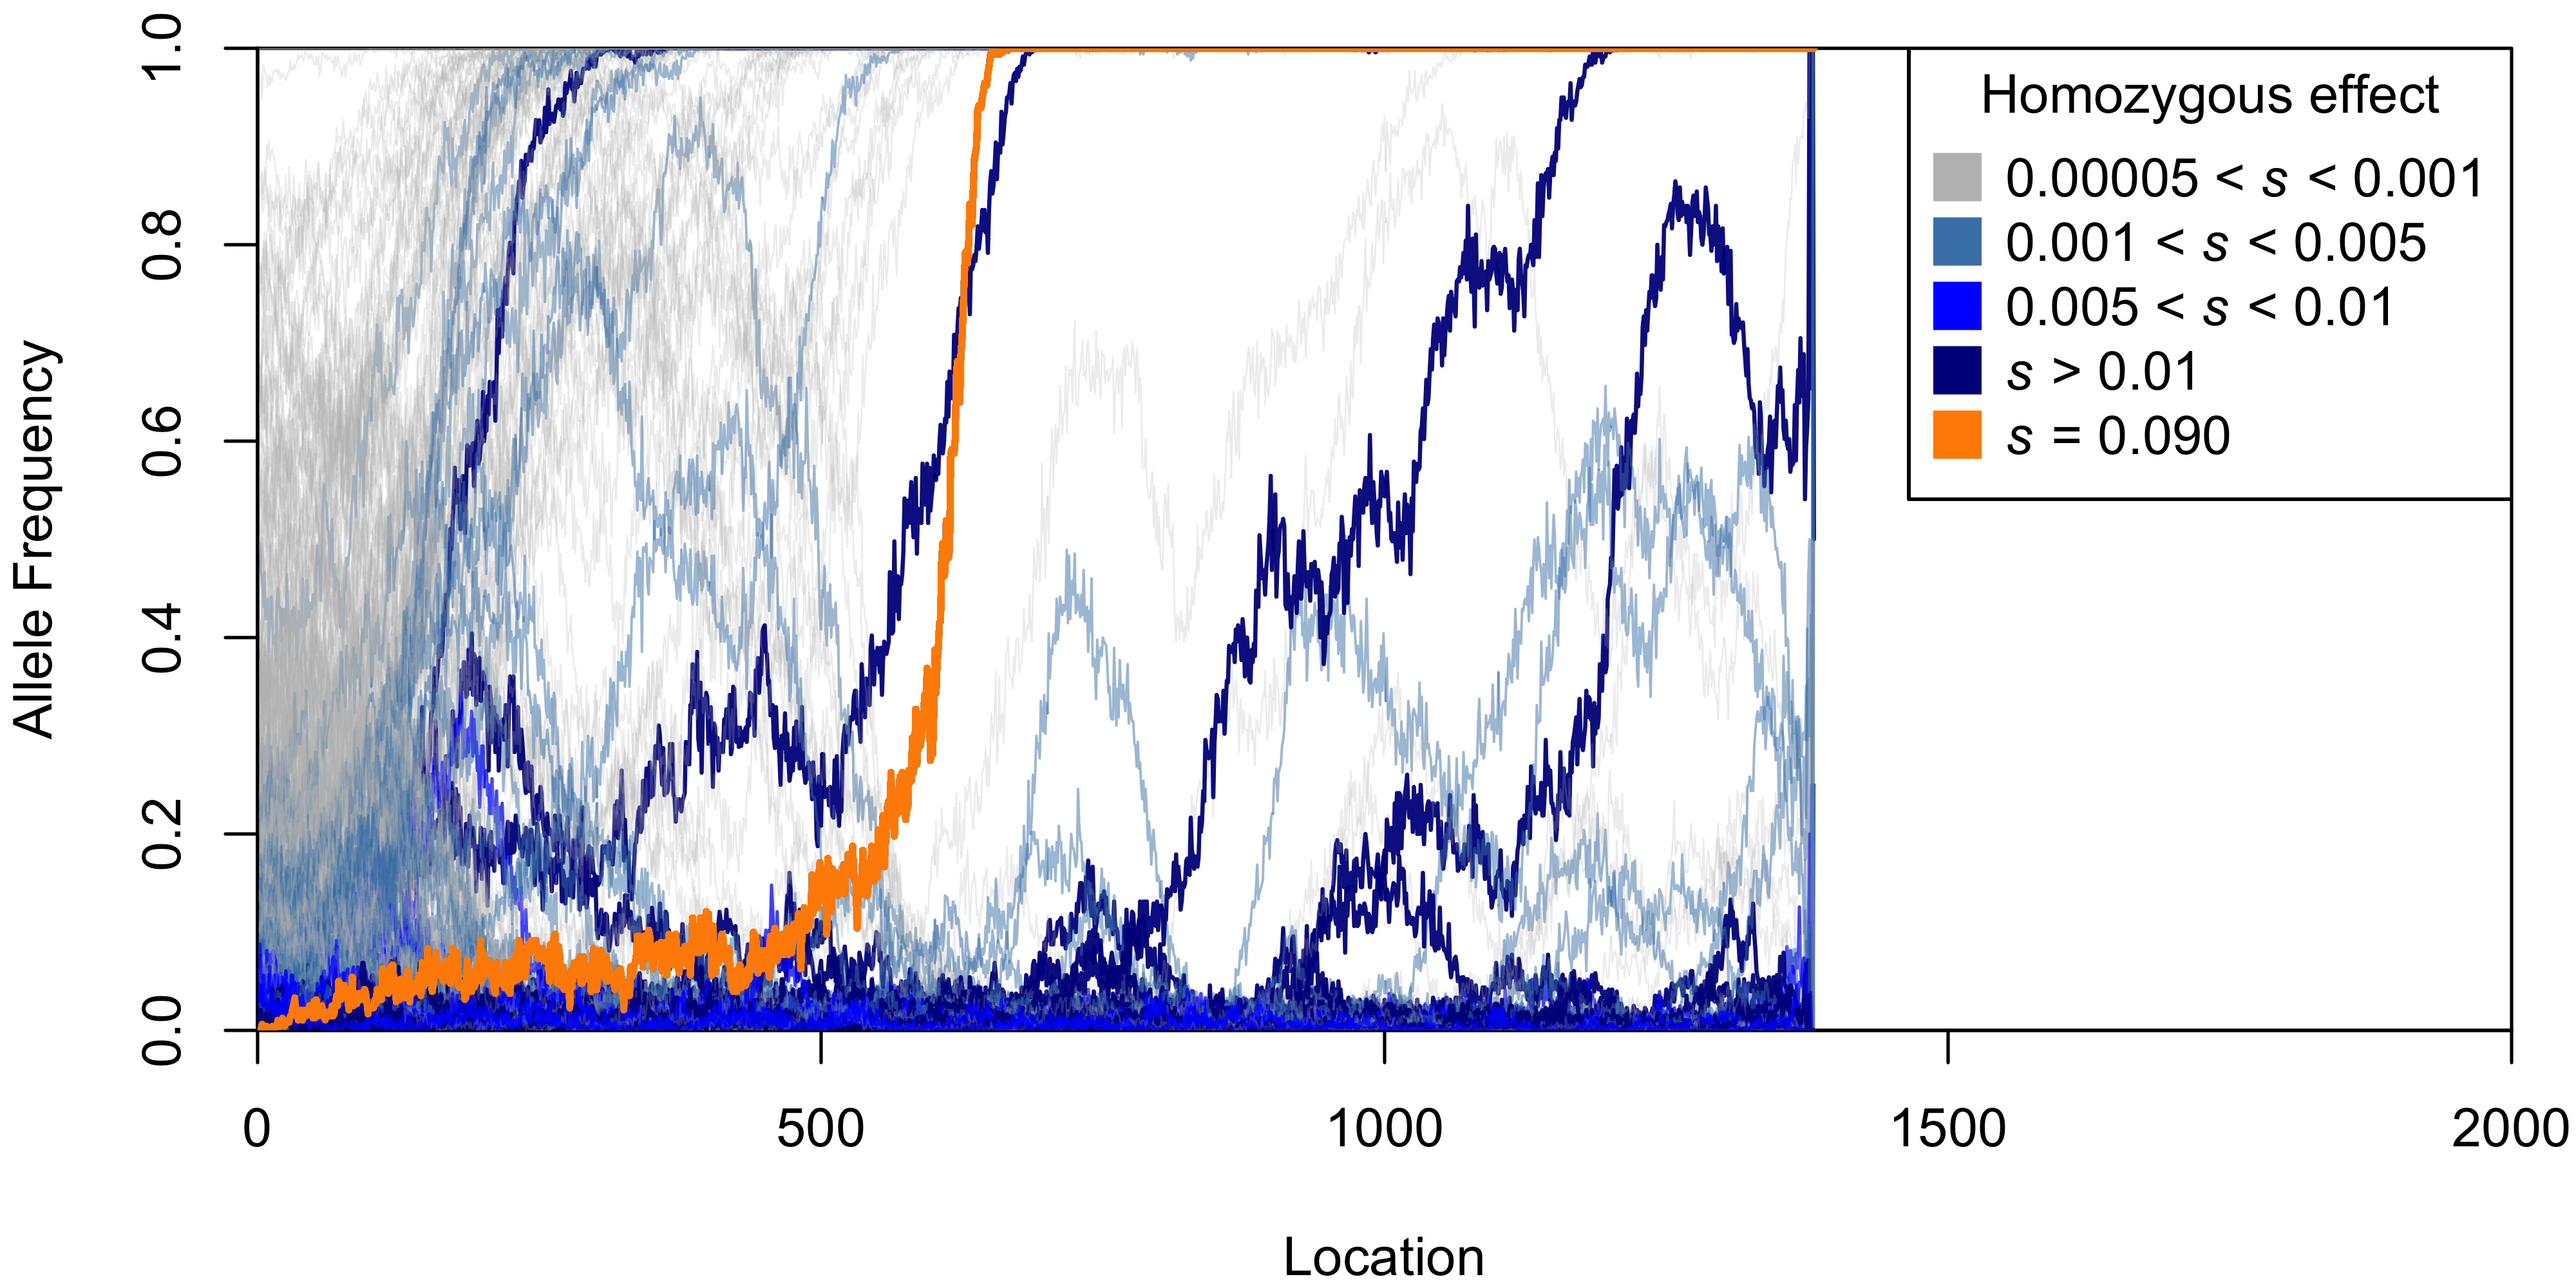
\includegraphics[width=1.0\linewidth]{Figures/example_allfreqs_color.png}}
\caption[~- Deleterious allele frequencies across the landscape.]{Snapshot in time of deleterious allele frequencies across the landscape, by homozygous effect size, \emph{s}. This example is at 250 generations after burn-in for the case of a leptokurtic dispersal kernel, with $U_D = 0.1$ and $b = 0$. This example was not randomly chosen, but selected to show that large effect loci can locally fix under these conditions. The locus indicated by the thickest orange line has an effect size of $0.0898$.}
\label{fig:allfreqs}
\end{figure}

% recovery rates in suppmat







%% add mike's point to discussion - in addition to the quanti trait redicing fitness and slowing expansion therefore reducing load, the same is true for more delet loci, i.e. load calcualted from one delet mut and multiplied up to more would overestimate the actual realized load

\section{Discussion}


%broadly start discussion for where our study fits into the literature of this field
%why no range limits are found
%compare to polechova and barton 2015
%could bring in relation to bridle et al 2010

Range expansions are unique demographic events that lead to an interesting suite of population genetic processes. These processes have been widely studied, yet the combination of both a heterogeneous environmental gradient and expansion load from deleterious mutations has not previously been investigated. Previous theoretical studies focusing independently on either the expansion load or adaptation along an environmental gradients predicted reduced fitness at the range edge. We find that these factors interact, so that the load at the expanding range edge is not as great as would be expected by a simple combination of the two. Both expansion load and local maladaptation to an environmental gradient reduce fitness at the range edge, but the mechanism of fitness reduction is important in the process of range expansion. Whether fitness is reduced due to local maladaptation or due to expansion load impacts the rate of range expansion, and therefore the rate of evolutionary rescue and thus the load that accumulates during expansion. This interaction is important for predicting the dynamics of modern range expansions due to natural phenomena or human-induced climate change. 

Our results corroborate previous studies, showing that expansion load accumulates at expanding range edges. Even though our simulation design differs from previous models investigating expansion load, we still find substantial load accumulating throughout the course of range expansion. The presence of hard versus soft selection can change the amount of expansion load accumulated \citep{Peischl:2013, Peischl:2015}, as can one- versus two-dimensional landscape models \citep{Peischl:2013}. Several other differences such as a range of mutational effects for deleterious alleles and continuous dispersal rather than a stepping-stone model might also contribute to the amount of expansion load.

%%We find an interesting interaction between migration load arising from an environmental gradient and expansion load arising from deleterious mutations in our simulations. The greatest expansion load ($39\%$) occurred in the absence of an environmental gradient. Rather than combining multiplicatively to further reduce fitness in edge populations, these factors instead interact to create a total load at the range edge that is not as bad as would be predicted. Steeper environmental gradients reduce expansion load, and higher deleterious mutation rates increase local adaptation to the environment. This effect would likewise have implications for 1-locus models of expansion load whereby it would be incorrect to assume an additive buildup of load when introducing more loci to a model.

%%We attribute this interaction to evolutionary rescue of one fitness component, allowed by the slower range expansion due to load in the other. Expansion across an environmental gradient is more difficult than in a homogeneous environment because local adaptation is impeded by the influx of maladaptive alleles from migrants \citep{Kirkpatrick:1997, Barton:2001, Polechova:2015}. This migration load alone can particularly reduce fitness at the range edge due to asymmetric migration from central populations \citep{Kirkpatrick:1997}. As the gradient steepens and increases the difficulty of local adaptation, fitness at the expanding edge decreases and expansion slows. This slower rate of expansion is key to the alleviation of expansion load because it provides increased time for evolutionary rescue and recovery from expansion load. When expansion is slowed, more migrants can reach the range edge, and population sizes can recover more quickly.

%%The fact that increasing deleterious mutations alone does not reduce expansion speed nearly as much as creating a steep environmental gradient explains the mechanism of the interaction of these two factors and emphasizes their significance. Expansion load that any given individual has accumulated would be equivalently detrimental to that individual's fitness regardless of where it existed on the landscape. The same is not true for the migration load that an individual might experience at the range edge. Maladaptation to the environmental gradient is changed if an individual is transplanted to a different location on the landscape. The population's survival is determined by total fitness, but the components of this fitness become meaningful when each changes the other. In our scenarios, increasing expansion load reduces total fitness at the range edge, therefore to survive and even exist, individuals must be more locally adapted. Successful expansion across a steep environmental gradient thus requires greater local adaptation than is otherwise needed in the absence of expansion load.

Our main result is that expansion load and the load due to local maladaptation interact. Local maladaptation at the range edge is not as severe in the presence of expansion load, and of an even greater effect, expansion load is not as severe in the presence of a strong environmental gradient causing local maladaptation. We believe that the dominant reasons differ for these two patterns of interaction. 

First, let us consider the improvement in the local adaptation at the range margin in the presence of expansion load. For a population to expand, the individuals at the expanding front must have an absolute fitness greater than one, on average. This means that a range margin will occur where absolute fitness drops below one. As a consequence, when there is greater load in one component of fitness, such as that caused by deleterious mutations across the genome, the population will not persist unless other fitness components are large enough to allow sufficient absolute fitness. Therefore, when expansion load is greatest, as occurs at the range edge, the fitness due to local adaptation must be higher in order for the population to have a large enough fitness to even exist. Note that this improvement in local adaptation is more a case of expansion load eliminating maladapted populations at the expanding front rather than a reduction in load. As a result, greater adaptation in the quantitative trait is found in the presence of expansion load.
%%This effect would likewise have implications for 1-locus models of expansion load whereby it would be incorrect to assume an additive buildup of load when introducing more loci to a model.

On the other hand, we also observe that expansion load can be greatly reduced in the presence of local maladaptation. In this case, we believe that there is an additional factor explaining this interaction.  In the absence of an environmental gradient, where the greatest expansion load accumulated ($39\%$), range expansion is mainly limited by dispersal ability. However, with local maladaptation caused by an environmental gradient, expansion is further slowed by the need for colonizing populations to adapt to the novel local environment. In fact, range expansion is slowed considerably more by a changing selective environment than by a high frequency of uniformly deleterious alleles (See figure \ref{fig:fitspeed}). As a result, the local maladaptation caused by a heterogeneous environment causes the rate of range expansion to slow substantially (Figure \ref{fig:speed}), which allows more time for evolutionary rescue of marginal populations. As range expansion slows, selection has more opportunity to reduce the frequency of deleterious alleles at the edge. Moreover, with slower expansion, high fitness alleles from the center of the range have more time to disperse toward the edge restoring genetic diversity at sites locally fixed for deleterious alleles by previous drift, and back mutation also has more time to generate beneficial diversity. 
%% Loren says delete all remaining sentences in this paragraph - repetitive
%% KJG agree - these repeat the same result described thoroughly above in this paragraph
%% REMOVED: In general, slower expansion ameliorates the conditions necessary for high expansion load at the range margin. Therefore, the local maladaptation caused by heterogeneous environments can reduce expansion load by slowing the rate of range expansion.

The mechanism altering expansion speed is a vital part of the process for these interactions to occur. When expansion is not slowed by the need to locally adapt and instead only by dispersal limitations, there is no expectation for a faster expansion to contribute to increased load. This explains the lack of further fitness reductions from increased expansion speed in our simulations with long distance dispersal. Instead, local adaptation at the edge was slightly reduced and expansion load less severe than in the Gaussian dispersal case, suggesting that this difference in dispersal models led to only slightly different amounts of expansion load accumulating given the different amount of connectivity between the core and edge. %%\citet{Fayard:2009} found that surfing was reduced in cases of long distance dispersal, substantiating this result. (\color{red} I think given our new interpretation of the results, Fayard no longer applies - will remove that part unless you think otherwise?\color{black})

Expansion load is attributed to the reduced efficacy of selection during expansion allowing detrimental mutations to accumulate, a result our study supports. The effect sizes of mutations underlying expansion load have important empirical implications, as many studies today aim to understand expansion load in humans after expansion out of Africa \citep{Lohmueller:2014, Lohmueller:2014b, Henn:2015,Henn:2015b, Gravel:2016}. Whether expansion load exists but is difficult to detect has been debated, and a full understanding of the selection coefficients across human (or other) genomes is lacking \citep{Hancock:2011, Lohmueller:2014, Simons:2014, Henn:2015, Henn:2015b}. We find an interesting difference in the make-up of expansion load between our two simulated cases of genome-wide deleterious mutation rates. While deleterious alleles of moderate and large effect are relatively rare, we find that they are responsible for the majority of expansion load. These alleles, which would otherwise tend to be purged or kept at low frequency by purifying selection, are able to increase in frequency on the expanding wave front. Interestingly, we find that in cases exhibiting faster range expansion, a larger proportion of expansion load comes from alleles of moderate and large effect, as purifying selection has less time to oppose the rise in frequency of strongly deleterious alleles.


\subsection{Implications, Caveats, and Future Directions}

%% come back to this para after figure out speed implications
Our finding that local maladaptation interacts with expansion load has broad evolutionary and ecological implications, including for studies of natural range expansions under climate change, invasive species, and conservation efforts \citep{Hunter:1994}. For example, highly invasive species are known for their rapid rate of spread (e.g., cane toads in Australia \citealt{Phillips:2006}), providing interesting opportunities to examine if and how these species accumulate expansion load. Conservation efforts that aim to reintroduce genetic diversity through assisted migration would clearly benefit edge populations in terms of reducing expansion load, but potential disruption to local adaptation is also a concern \citep{Aitken:2013}. Finally, both expansion load and migration load are likely to affect climate-change induced range shifts. Rapid climate change would necessitate fast range expansion. Therefore, expansion load may be increased and local adaptation decreased, leaving struggling populations subject to stochastic extinction events. If the speed of climate change is not too fast, however, populations adapting as they move over space may reduce any potential impacts of expansion load. 

There are several biological features of organisms and their environments that we did not consider in our simulations due to the vast computational resources already required, but these merit future investigation. Our simulations allowed for individuals to self-fertilize when mates were limited, but this is not possible in many species. The inability to self-fertilize could slow range expansions, leading to a reduction in expansion load. Other effects can similarly reduce fitness in small edge populations. Allee effects \citep{Taylor:2005} or aggregating dispersal behavior that discourages colonization of empty habitat \citep{Altwegg:2013} would slow expansion, as might dispersal barriers or increased encounters with antagonistic species (e.g. competitors, pathogens) \citep{Case:2005, Kubisch:2013}. It would be interesting to consider species with overlapping generations, where previously established individuals may block immigration into patches at carrying capacity (i.e. a priority effect, \citealt{Atkins:2010}). Priority effects could slow replacement of initial colonizers at the range edge, impeding genetic rescue and increasing the persistence of expansion load away from the edge. Some factors that could speed expansion beyond rates seen in our model and lead to increased expansion load include greater long distance dispersal or increased fecundity. We found that simulations with fecundity halved ($3.5$ vs. $7$, data not shown) exhibited much less expansion load and higher fitness in edge populations. Thus, increasing fecundity allows populations to persist at lower mean fitness and thus accumulate more load. Finally, other factors could result in complex, less predictable effects.  Local adaptation likely involves multiple quantitative traits adapting over similar or different environmental gradients, with potentially complex interactions that merit future investigation.

A potentially key evolutionary component of range expansions not included in our model is the evolution of dispersal ability. Increased dispersal is always expected to evolve at expanding range margins \citep{Hargreaves:2014}. Interestingly, increased dispersal is expected theoretically and found empirically even during expansion across environmental gradients or with expansion load alone \citep{Henry:2015b}. However, increased dispersal also steepens the perceived slope of a given environmental gradient, which can eventually slow or even temporarily halt range expansion until edge populations evolve to overcome initial maladaptation (e.g. \citealt{Phillips:2012}). Therefore it is unclear how dispersal evolution would affect the results presented in the current study.


\subsection{Conclusions}
% closing paragraph on broader implications

Our results support those of previous studies finding that expansion load via the surfing of deleterious alleles reduces fitness in expanding populations \citep{Peischl:2013, Peischl:2015, Peischl:2015b}. We show this under biologically realistic conditions, bolstering evidence that allele surfing may, indeed, cause expansion load in nature. Our results are also in agreement with those of previous studies showing that on an environmental gradient, migration load reduces fitness in expanding populations \citep{Kirkpatrick:1997, Bridle:2010, Polechova:2015}, though we did not see any cases of stable range limits as a result of local maladaptation or expansion load. We highlight the mechanism of interaction between local maladaptation and expansion load. Local maladaptation feeds back to reduce the speed of expansion and thus allows for increased evolutionary rescue throughout range expansion. Finally, we demonstrate that faster range expansion leads to a larger contribution of moderate and large effect deleterious alleles to expansion load. These contributions significantly advance theory on the genetics of range expansion towards meaningful predictions and interpretations for studies of natural populations.




%%% Local Variables:
%%% TeX-master: "thesis"
%%% TeX-PDF-mode: t
%%% End:

\chapter{Recommendations for utilizing and reporting population genetic analyses: The reproducibility of genetic clustering using the program \textsc{structure}}
\label{chap:reproducibility}

\section{Summary}

Reproducibility is the benchmark for results and conclusions drawn from scientific studies, but systematic studies on the reproducibility of scientific results are surprisingly rare. Moreover, many modern statistical methods make use of ‘random walk’ model fitting procedures, and these are inherently stochastic in their output. Does the combination of these statistical procedures and current standards of data archiving and method reporting permit the reproduction of the authors’ results? To test this, we reanalysed data sets gathered from papers using the software package STRUCTURE to identify genetically similar clusters of individuals. We find that reproducing STRUCTURE results can be difficult despite the straightforward requirements of the program. Our results indicate that 30\% of analyses were unable to reproduce the same number of population clusters. To improve this, we make recommendations for future use of the software and for reporting \textsc{structure} analyses and results in published works.

\section{Introduction}
The reproducibility of scientific research is fundamental to maintaining scientific rigor and advancing science (Price 2011). Full experimental replication provides the most thorough means of verifying published empirical results, but this approach can be impractical due to the difficulty in obtaining identical samples and large financial and time commitments (Peng 2011). Diminishing costs and advancing technology have resulted in a plethora of large genetic data sets, while at the same time, there has been an increase in the complexity of software applications. A previous investigation into the reproducibility of microarray studies found that few were fully repeatable, as many suffered from ambiguity in the methods, discrepancy in the results, and lack of available data or software (Ioannidis et al. 2009). Maintaining the rigor of today’s scientific research may therefore prove a more difficult task than expected, as both the empirical results and the often complex analyses need to be reproducible. Efforts to encourage and implement data archiving and sharing are expanding, and these create the opportunity to test the validity and reproducibility of scientific results (Whitlock et al. 2010).

Reproducing results within the field of molecular ecology is especially difficult because biological samples are unique to their particular place and time, and subsequent samples may reflect different ecological or evolutionary forces (Wolkovich et al. in press). Researchers therefore tend to test the same overarching hypothesis with samples from different taxa and locations, in the hope of arriving at a more general and repeatable pattern. However, drawing broad conclusions from the results of many studies is ineffective when the results of the individual studies cannot be reproduced from their underlying data. It is thus essential to test the reproducibility of statistical analyses at the level of individual papers as well. To examine how well we could recreate the results from typical molecular ecology studies, we investigate, as an example, the reproducibility of studies that used genotype data to identify genetically similar clusters of individuals with STRUCTURE (Pritchard et al. 2000). Many studies use clustering results based on STRUCTURE to perform further analyses, making it an important foundation upon which inferences are built. We ask whether (i) archived data sets are sufficiently complete and well annotated that they can be reused, (ii) published articles specify all the methodological details necessary to reproduce the analysis, and (iii) where possible, the same conclusions can be reached by reanalysing the archived data. Although reproducibility has many different aspects, we use it here to mean the agreement between results obtained through analysing identical data sets using the same analytical method but under different conditions (different observers, computers and starting points in computer algorithms). We reanalysed 23 articles from 2011 that used STRUCTURE to infer genetic clustering and also checked the level of data completeness and methodology reporting in an additional 37 articles.

\section{Methods}
\subsection{Obtaining Datasets}
We gathered \textsc{structure} data sets associated with 23 papers published in 2011: 21 from Molecular Ecology, and two from the journal PLoS One. Data were obtained from the online data repository Dryad (Dryad Digital Repository) in November 2011, NCBI GenBank, or from the supplementary material accompanying the paper. With one exception, we excluded papers where data were archived on GenBank due to the difficulty of compiling individual accessions into the correct format for \textsc{structure}.

For a broader assessment of data set completeness and methods reporting, we also included 37 data sets obtained by contacting the authors of original research papers published in PLoS One, PLoS Genetics and BMC Evolutionary Biology and collected as part of a separate study (T.H. Vines et al., unpublished data).

\subsection{The Program \textsc{structure}}
The freely available Bayesian clustering program \textsc{structure} (Pritchard et al. 2000) is the most commonly used application to infer population structure, with over 5000 citations in Web of Science as of June 2012. \textsc{structure} uses multilocus genotype data to describe and visualize population structure based on allele frequencies of the data.

\textsc{structure} is capable of analysing a variety of genotype data, including both codominant markers (microsatellite and single nucleotide polymorphism, SNP; Pritchard et al. 2000) and dominant markers (amplified fragment length polymorphism, AFLP; Falush et al. 2007). The model uses Markov chain Monte Carlo (MCMC) simulations to estimate the group membership of each individual, assuming Hardy–Weinberg and linkage equilibrium within groups, random mating within populations and free recombination between loci (Pritchard et al. 2000). Due to the random walk characteristic of the MCMC methods, \textsc{structure} outputs are not expected to produce identical results, yet the approach should be robust enough to yield identical conclusions when reproduced. The program is initiated with a required text file containing individual genotype data and labels as well as optional information on population assignment, sampling sites or locus names. The user specifies several essential parameters regarding the ancestry
model, the allele frequencies model, the length of the burnin (initial runs of the simulation during which data are not retained to ensure results are not dependent on initial conditions), length of run time (number of MCMC repetitions during which data are retained), the number of independent replicates of each set of parameters and the range of number of clusters (K values) to be tested. These can be specified directly in the graphical user interface or in a separate text file when run in the command line. In addition, it is possible to specify extra parameters, mainly regarding the Markov chain process as well as a sampling location prior. The details of the model are described by Pritchard et al. (2000, 2007) and Falush et al. (2003, 2007).

\textsc{structure} outputs are typically analysed to infer the optimal \emph{K} by one or a combination of methods. In the method described in Pritchard et al. (2000), the optimal \emph{K} is chosen by plotting the log probability of the data (referred to as ln Pr(X|K) in \textsc{structure}’s manual, Pritchard etal. 2007) against a range of \emph{K} values and selecting the \emph{K} with the highest ln Pr(X|K) or the one after which the trend plateaus, while also taking into account the consistency of the groupings across multiple runs with the same K. An alternative method, described by Evanno et al. (2005), formalizes an ad hoc approach based on plotting the secondorder rate of change in ln Pr(X|K) for successive Ks (referred to as DK) against a range of \emph{K} values, and selecting the true \emph{K} based on where the maximal value of this distribution occurs. As emphasized in the \textsc{structure} manual (Pritchard et al. 2007), selecting the optimal \emph{K} can be quite a subjective procedure and is best inferred when the biology and history of the organism are taken into account. Replicate \textsc{structure} runs can be combined using the software programs \textsc{clumpp} (Jakobsson \& Rosenberg 2007) and \textsc{structure harvester} (Earl \& von Holdt 2011). Bar plots depicting the ancestry proportions (or membership coefficients, Q) of individuals in each cluster can then be created, for example with the software DISTRUCT (Rosenberg 2004), to visualize the population clusters.

\subsection{Analysing Data Sets}
We followed procedures for analysis as described in the methods section of each publication and used default settings for parameters that were not specified. Several publications performed multiple \textsc{structure} analyses, which we counted independently for a total of 34 analyses. We made use of the Bioportal computing resource (https://www. bioportal.uio.no/; Kumar et al. 2009) or local desktop computers. Output was compiled with \textsc{structure harvester} and processed following the authors’ description, including CLUMPP analysis where appropriate. We first assessed whether we could reproduce the \emph{K} values from the original study based on the methods used by the authors. Then, whenever possible, membership coefficient bar plots were visually compared by multiple authors of the present study to assess whether our results were a true reproduction of the original results. When we concluded the same value of \emph{K} as the authors, we deemed the analysis as reproducedunless the membership coefficient bar plots showed strikingly different results.

For the broader survey of data set completeness, we evaluated whether the sample size and number of loci described in the paper matched the obtained data set from both the data sets obtained from online material (23 studies) and email correspondence (37 studies). To check the overall standards for reporting parameter settings within either the methods section or in a supplemental file, we also recorded the number of ‘essential’ parameter settings (range of \emph{K} values tested, length of burn-in, length of MCMC repetitions, number of independent replicates, the admixture model and allele frequencies model) given in the paper or supplemental material for all of the above analyses.

\section{Results}
Of the 23 papers, we attempted to reanalyse using data from supplementary materials or online repositories, two papers did not have archived data present at the time, making their reanalysis impossible. Three papers (13\%) provided data where the number of individuals and/or loci specified in the publication did not match those present in the data set, or the authors performed their \textsc{structure} analysis on an unspecified subset of the archived data. Of these 23 papers, three selected \emph{K} using the Pritchard method (Pritchard et al. 2000), seven used the Evanno method (Evanno et al. 2005), eight used a combination, one used a nonparametric Wilcoxon test, two did not specify their method, one used no standard method and rather utilized \emph{K} = 2 to identify hybrid individuals and one discussed a comparison of two \emph{K} values obtained in a previous study. We therefore also did not assess the reproducibility of these final two papers, leaving 19 papers (containing 30 analyses) that we attempted to reproduce. See Table S1 (Supporting information) for full characteristics of all analyses.

We were able to reproduce the authors’ inference of \emph{K} for 70\% (21 of 30) of the analyses (Figure ~\ref{fig:repro-1}). All of the successfully reproduced data sets consisted of microsatellite genotypes. In general, microsatellite data sets were analysed using longer burn-in and MCMC run lengths as well as more independent replicates; however, there was no significant difference in an overall proxy for run length
([length of burn-in + length of MCMC repetitions] 9 number of independent replicates) between 
analyses that were reproduced and those that were not (t = 0.0617, d.f. = 13.564, P-value = 0.95). 
Comparing these parameters individually, we found a trend of longer burn-in (t = 1.8706, d.f. = 26.991, P-value = 0.072) 
but not of more MCMC repetitions (t = 1.6537, d.f. = 21.677, P-value = 0.11) or an increase in the 
number of independent replicates (t = 1.1442, d.f. = 7.511, P-value = 0.29) for reproduced studies. 
Comparison of the \emph{K} values chosen by the original authors versus our reanalysed \emph{K} results 
showed a significant correlation of 0.5934 (t = 3.9703, d.f. = 29, Pvalue = 0.0004; Figure ~\ref{fig:repro-2}).

\begin{figure}[]
\centering
\makebox[\textwidth]{
        \includegraphics[width=1.0\linewidth]{Figures/repro_fig1.pdf}}
\caption{Results of \textsc{structure} reanalyses. Initial branching arrows show the numbers of analyses resulting in different outcomes at the point of selecting a \emph{K} value. The subsequent arrows show the numbers of analyses successfully reaching the point of matching membership coefficients. Size of arrowheads is proportional to number of analyses present. *When \emph{K} was not inferred, we attempted to match membership coefficients across all \emph{K} values (still only counted as 1 analysis). **When \emph{K} was not reproduced, we compared membership coefficients at the authors’ chosen \emph{K}. ***For incomplete data, analyses could not be run.}
\label{fig:repro-1}
\end{figure}

We also assessed the completeness and description of all 60 data sets that we obtained and found 35\% to be either incorrectly or insufficiently described by the authors. We found that 17 data sets did not match the description given in the paper, most typically because the data contained a different number of loci or individuals than suggested by the paper. Lastly, four papers did not give any clear description of the number of individuals, loci or both used in their \textsc{structure} analysis, making it impossible to judge how well the archived data matched the data analysed by the authors.

Authors’ descriptions of the essential parameters used to run \textsc{structure} varied markedly, ranging from 0 described parameters to a maximum of 6 (median = 6). We found a significant difference in number of essential parameters between two of the journals (t = 3.31, d. f. = 40.27, P-value = 0.015), with Molecular Ecology having a mean of 5.7 parameters specified and PLoS One 4.6 (PLoS Genetics, 4.7 and BMC Evol. Biol., 4.8). Overall, length of burn-in ranged from 1000 to 50 000 000 (median = 50 000), while MCMC repetitions ranged from 10 000 to 500 000 000 (median = 450 000). Independent replicates ranged from 3 to 100 (median = 10).

\begin{figure}[]
\centering
\makebox[\textwidth]{
        \includegraphics[width=1.0\linewidth]{Figures/repro_fig2.pdf}}
\caption{Comparison of \emph{K} values for original studies versus reproduced studies. Dotted line indicated the 1:1 line, points are jittered for better visualization.}
\label{fig:repro-2}
\end{figure}

\section{Discussion and Recommendations}
Reproducibility is a foundation of scientific research. The widespread application of \textsc{structure} makes it an ideal case study to test the ability to reproduce molecular ecology results that rely on large data sets and complex algorithms. As \textsc{structure} results often serve as the underpinnings for further analyses and conclusions within a study, it is important to assess whether the implementation of the program, subsequent analysis and associated conclusions are properly reported and can be reproduced.

We find that reproduction of \textsc{structure} results can be difficult to achieve, despite the straightforward input requirements of the program (a genotype file and two parameter files). Our results show that 30\% of analyses are not reproducible. A large factor in the failure to reproduce these analyses was the availability of data in a form that could be readily understood by researchers not familiar with the study system. Had we included studies with no data available as the starting point for our reanalysis, our assessment of failure to reproduce would have been even higher, particularly for journals without a strongly enforced data archiving policy (see T.H. Vines et al., unpublished data for further discussion of data accessibility).

We recognize that assessing reproducibility is inherently difficult. Our main evaluation criterion (same \emph{K} value) is only a small part of full reproducibility of these studies, but the most objective one. Furthermore, it is difficult to disentangle the nonreproducibility caused by the stochastic nature of the program from that caused by both discrepancies in data sets available versus those used by authors and their reported methods. The trend of longer burn-in lengths in reproduced studies suggests that at least a portion of the poor reproducibility of some studies is due to the inherent stochasticity of the Monte Carlo approach itself. In at least one case, we can attribute our failure to reproduce the study to insufficiently described, complex analyses performed; however, there seemed to be no other outstanding characteristics of nonreproducible studies. It is important to note that although \textsc{structure} is the most commonly used program, in some instances, other methods
may be more appropriate for a given data set. For example, performing a PCA allows examination of variability within clusters, other Bayesian methods such as the program \textsc{instruct} (Gao et al. 2007) allows inbred genotypes to be used, \textsc{tess} (Chen et al. 2007) utilizes spatial information, and \textsc{baps} (Corander et al. 2003, 2004, 2006; Corander \& Marttinen 2006; ) aids in detection of admixed individuals. Using the right program is not only essential to drawing correct conclusions, but may also improve reproducibility of results. Further discussion of additional approaches can be found in Latch et al. (2006) and Franc ̧ois \& Durand (2010).

In addition, we may have judged a study to be nonreproducible despite differences in the final results that may or may not have biological significance. The correlation between original and reproduced \emph{K} values implicates this, yet there is still clearly room for improvement. With such widespread use within its field, it is important that users of \textsc{structure} properly implement the software, regardless of whether or not they possess a full understanding of the algorithm underlying the analysis. To ensure that published results can be reproduced, we make the following recommendations for future users of the program. Although our study is specific to \textsc{structure}, many of these recommendations are applicable to other types of analysis.

1 For archiving purposes, authors should be encouraged to provide the final version of both the genotype and parameter files. We propose that authors archive genotype data from all individuals. If only a subset was used in the analysis, these individuals should be clearly identified in the same file so that this information is retained. The parameter files include all the settings used in the analysis, hence archiving the entire file avoids any confusion regarding use of default settings when not explicitly stated by the authors. When using the graphical user interface version of the software, the parameters can be exported from the program in text format for archiving purposes.

2 Authors should ensure that burn-in and run lengths are sufficient. We found remarkable variation in parameters affecting the computational demands of the analysis (burn-in time, MCMC repetitions, and replicate runs). Though we found no significant difference between an overall proxy for run length and reproducibility and only a slight trend individually for burn-in time, given the advances in computing power, we feel that the proposed minimum requirements, dating back to the software’s advent more than a decade ago, should be increased. It is difficult to set a standard, as variability across data sets in the number of loci, their levels of polymorphism, and the amount of population structure present all also contribute to the program’s ability to successfully detect the appropriate \emph{K} (Rosenberg et al. 2001; Latch et al. 2006; Gao \& Starmer 2007). We would advise a minimum of at least 100 000 burn-in iterations and MCMC repetitions for each run, and much longer burnin will be required for some data sets. Comparing a range of run durations may help to determine the appro-priate run length, and it is always advisable to choose a longer burn-in and run length. To confirm that burn-in is adequate, it is also important check for convergence in values of summary statistics (particularly a, F, D, and the likelihood) that are estimated by the program, as recommended in the \textsc{structure} manual (Pritchard et al. 2007). Additional independent replicate runs are of great importance as they limit the influence of stochasticity and increase the precision of the parameter estimates. That is especially true when using the Evanno method, which requires an estimate of variance. In at least one reanalysis we performed, only five replicate runs were used, which may explain the failure to reproduce results (the chosen K) in this particular study. We recommend 20 replicates as used by Evanno et al. (2005).

3 Proper reporting of the methods used to analyse \textsc{structure} results is vital for inferring K. Whether the method outlined by Pritchard et al. (2000) or by Evanno et al. (2005) or both are used to select \emph{K} should be clearly stated, as well as any biological factors that have influenced the choice of K. Special attention should be given to the comparison of \emph{K} = 1 versus greater values, as the Evanno method is not capable of performing this comparison. We advise that results are reported in the form of the graph of the natural logarithm of the likelihood of the data given \emph{K} (if the Pritchard method was used) and the DK graph (if the Evanno method was used) as well as the bar plot(s) showing individual assignments for the given \emph{K} or comparison across plausible \emph{K} values. Ideally, for full reproducibility of a study, membership coefficients for each individual should also be provided. These results should be examined within each replicate to determine how much stochasticity is present before runs are averaged, as well as after averaging all replicate runs.

\section{Conclusion}
A substantial proportion of \textsc{structure} results were not reproducible, despite the relative simplicity of the procedure, requiring only a genotype file and associated parameter settings. Our recommendations on how to archive data sets analysed with \textsc{structure} should reduce the component of nonreproducibility due to uncertainty of parameter choice or lack of clarity in the data analysed, but some discrepancies will no doubt still persist. We hope that scientists will increasingly acknowledge the concept of scientific reproducibility in the future and be aware of practices they can enact both for better data archiving and better implementation of other similar programs in their analyses.

%%% Local Variables:
%%% TeX-master: "thesis"
%%% TeX-PDF-mode: t
%%% End:

\chapter{Conclusion}
\label{chap:conclusions}

The field of population genetics has grown by leaps and bounds since its advent. The rapid advancement of genetic and genomic techniques for acquiring data from every organism imaginable is a testament to this growth, as well as a cause. The insights allowed through these advances have greatly informed all aspects of evolutionary biology today. Even though I have not presented new data from natural organisms, my thesis work, and all theoretical work, relies heavily on information collected by evolutionary biologists through the years. We gain a great deal of knowledge by creating models of the natural world where alteration of specific factors can be controlled and investigated. Models that can be based in reality using parameters we know to be accurate to biology not only improve understanding of processes, but also their likely impact on real world populations.

I have presented four quite different projects within my thesis, each building upon the bounty of existing knowledge in the field of evolutionary biology. In \Chapref{effectivepopsize}, I tested the accuracy of methods designed for estimating effective population sizes. Out of a range of existing studies, I found that two methods perform best. I also found that their best performance varied across different demographic scenarios of migration among populations. This lends credit to the proposition made throughout my thesis, that knowing the demographic history of populations is both useful and necessary to make proper evolutionary inferences from data.

In \Chapref{heterogeneouslandscapes}, I simulated cases of range expansions over environmental gradients that varied over space in terms of patchiness and steepness. Varying the genetic architecture of the trait underlying adaptation to the environment showed different abilities of populations to adapt and expand their ranges. Two qualitatively different regimes resulted whereby expansion could succeed from either many small effect alleles or few large effect alleles. Intermediate between these two regimes, expansion was more limited, indicating that this may be the parameter space for which adaptation is most difficulty. Though the upper bound of the mutation rates included may be unrealistic, this result provides impetus for future investigation of the interaction between mutation numbers, effect sizes, and the scale of change in the environment.

In \Chapref{expansionload}, we examined range expansions with combinations of conditions generating either or both expansion load and local maladaptation to an environmental gradient. We found an interesting interaction between these two factors, whereby the fitness reduction cause by expansion load accumulating at expanding range fronts reduces population fitness. In the presence of steep environmental gradients, a fitness cost is already incurred as populations attempt to adapt to the local environment. When combined, these effects compound and lead to the extinction of populations at the range edge, instead leaving behind a different range edge or more locally adapted individuals. Because any lower degree of local adaptation would combine with expansion load to generate populations with fitness levels below those of persistence, those populations simply no longer exist, and local adaptation is improved at the range edge at a cost of slower range expansion. Investigating further parameter space around these simulation as well as investigating other biologically realistic possibilities such as evolution of dispersal provide ample future directions for this research.

In \Chapref{reproducibility}, we performed a reproducibility study on published datasets using the analysis method \textsc{structure}. We found that the same biological result of $K$ values could be reproduced in 70\% of studies. However, if we measure this success at the starting point of acquiring the datasets for which reanalyses were performed, this percentage would decrease greatly. These results are nonetheless promising, as they indicate the successful repeatability of a stochastic genetic analysis method. It would be interesting to conduct a similar reproducibility study today, since the standards for data archiving have greatly improved in the four years since publication of this study.

Each of these projects has its own limitations as well as its own implications. An important running factor throughout these disparate works is the immense amount of work performed, yet the small realm of evolutionary studies that are informed. This reflects the breadth of evolutionary biology and the immensity of knowledge we have yet to understand as scientists. The simulation studies in \Chapref{effectivepopsize, heterogeneouslandscapes, expansionload} each investigate a specific range of parameter sets, as computational resources are limited, and the values deemed most important and relevant were investigated. We have gained knowledge that, however, could not be obtained from analytical models that might better describe a range of important parameters for examining a given population process. In particular, \Chapref{heterogeneouslandscapes, expansionload} have used spatially explicit simulations over large scale landscapes to investigate range expansions. Such an approach is computationally intensive and has not been used in previous studies of range expansion on this scale. The biological realism introduced by this approach has let us investigate specific questions of value, especially in \Chapref{heterogeneouslandscapes} where the structure of the landscape is a key aspect under investigation. This approach has been made publicly available for others to use in future studies and will hopefully allow continued biological insight into population genetic processes occurring in large scale landscapes.

The simulated data generated from \Chapref{effectivepopsize} was designed to test biological scenarios most relevant to scenarios occurring during estimation of effective population size in natural populations. Testing all methods available at the time on this range of data was the first fair comparison method to method. As new methods for estimating effective population size have been developed, this data will continue to be valuable in further comparisons. Since publication of \Chapref{effectivepopsize}, a new method \citep{Hui:2015} has also been created for which I hope to test across all scenarios already investigated in my study. A new study has also performed a comparison across a subset of these methods to test their performance in a different range of biological scenarios as well as with differing effects of genetic markers on these inferences \citep{Wang:2016}. This is a trend that may be best seen for methods estimating effective population size. Several previous studies have presented assessments of method performance \citep{Ryman:2013, Neel:2013, Holleley:2013, Hoehn:2012, Barker:2011}, and author who develop these methods generally present an evaluation of their approach upon publication. This method testing is vital, but often lacks consistency in comparison across methods and datasets, resulting in a comparison of apples to oranges. Methods testing can be difficult and time-consuming, however, and no author is generally able to predict all situations for which their method may be applied. The burden thus rests on researchers applying these methods to ensure that they are meeting the appropriate assumptions of the method, or to first test how applying a method may be biased in their biological scenario.

A great effort which has yet to come to fruition, is the idea to maintain an online database of simulated data for methods testing. This would standardize comparisons from different researchers to the same test dataset. Simulated data allows accurate assessment of analysis results because the true parameters or biological answers within the simulated data are known. This would also increase the ease of methods testing, as authors do not have to continually generate their own test datasets. Furthermore, researchers applying a dataset to a new scenario that may be assumption-violating would be able to find equivalent simulated data and test the method themselves in order to understand how useful it may be. The finalization of this sort of database would be a great boon to advancing population genetic analyses, particularly as more and more genetic analyses methods are formulated. As more data, simulated and natural, continues to be archived at publication and resources for long-term storage and access to data grow, the state of data availability is optimistic for evolutionary biology.

With the relative ease of acquiring genetic data, population genetics is beginning to face a larger problem of learning new ways to analyze large genomic datasets. No longer is it the case that we lack in data; we now lack the ability to fully make use of this data in many cases. Until recently, the majority of existing methods functioned only for small sets of loci. Genomic advances now provide researchers with abundances of data that can overload analysis methods. A through understanding of the value gained from additional loci past a certain point is lacking, but if we operate under the assumption that more data is always better, then valuable information may be lost when methods can not accommodate all of the data. A temporary solution used by some researchers in applying a method designed for few loci is simply subset their data. Subsetting is often a non-optimal solution, because multiple analyses of different subsets are then still necessary to ensure no bias has unknowingly entered the subset data. Fortunately, more and more methods continue to be developed for handling genomic data on large scales; for example analyses of population structure have greatly advanced \citep{Raj:2014,Bradburd:2016, Petkova:2015}.

Major questions still remain to be answered in evolutionary biology. Particularly relevant to my projects on adaptation during range expansion and under differing genetic architectures, as well as to the topic of large scale data analysis, is the question of how many loci contribute to local adaptation. Detecting small effect loci in real datasets is extremely difficult, compounded by the statistical problem of comparing across huge sets of loci. Through these simulation studies, I hope that I have contributed to interesting avenues of research that will continue to be investigated. From \Chapref{expansionload}, we saw that the effects of multiple loci on fitness and adaptation did not combine multiplicatively, but instead interacted. This both lends credit to as well as points out the faults in learning biology from simplified models. Our model clearly improved upon any using simply one locus. Were one to predict the effects on population survival during range expansion by extrapolating from a one-locus model, the result would be highly unrealistic, as adding more loci creates the potential for ever-increasing interactions. Such interactions are likely to be rife throughout biology, and understanding these interactions through controlled simulation experiments becomes valuable for creating a strong foundation of predictions to be tested in real world data. In combination, theoretical and biological insights become the most valuable for advancing our knowledge of evolution, and I hope that the results of my work lead to worthwhile investigations of population genetic processes in species alive today.


%% For you conclusions chapter, you might want to discuss how range shifts rather than range expansion could change the predictions. of this and the previous chapter.   Add in some of the ideas from your post-doc proposal, perhaps.
%% evolution of dispersal
%% seed vs pollen dispersal
%% range shifts vs pure range expansions


%% stickleback NE and NB ne estimation method

\formatbibliography
\bibliographystyle{refstyle}
\bibliography{refs-thesis}

\formatappendices
\chapter{Supplementary Information to \Chapref{incredible-discovery}}

\section{A section heading}


\end{document}

%%% Local Variables:
%%% TeX-master: t
%%% TeX-PDF-mode: t
%%% End:
